\documentclass[twoside]{book}

% Packages required by doxygen
\usepackage{calc}
\usepackage{doxygen}
\usepackage{graphicx}
\usepackage[utf8]{inputenc}
\usepackage{makeidx}
\usepackage{multicol}
\usepackage{multirow}
\usepackage{textcomp}
\usepackage[table]{xcolor}

% Font selection
\usepackage[T1]{fontenc}
\usepackage{mathptmx}
\usepackage[scaled=.90]{helvet}
\usepackage{courier}
\usepackage{amssymb}
\usepackage{sectsty}
\renewcommand{\familydefault}{\sfdefault}
\allsectionsfont{%
  \fontseries{bc}\selectfont%
  \color{darkgray}%
}
\renewcommand{\DoxyLabelFont}{%
  \fontseries{bc}\selectfont%
  \color{darkgray}%
}

% Page & text layout
\usepackage{geometry}
\geometry{%
  a4paper,%
  top=2.5cm,%
  bottom=2.5cm,%
  left=2.5cm,%
  right=2.5cm%
}
\tolerance=750
\hfuzz=15pt
\hbadness=750
\setlength{\emergencystretch}{15pt}
\setlength{\parindent}{0cm}
\setlength{\parskip}{0.2cm}
\makeatletter
\renewcommand{\paragraph}{%
  \@startsection{paragraph}{4}{0ex}{-1.0ex}{1.0ex}{%
    \normalfont\normalsize\bfseries\SS@parafont%
  }%
}
\renewcommand{\subparagraph}{%
  \@startsection{subparagraph}{5}{0ex}{-1.0ex}{1.0ex}{%
    \normalfont\normalsize\bfseries\SS@subparafont%
  }%
}
\makeatother

% Headers & footers
\usepackage{fancyhdr}
\pagestyle{fancyplain}
\fancyhead[LE]{\fancyplain{}{\bfseries\thepage}}
\fancyhead[CE]{\fancyplain{}{}}
\fancyhead[RE]{\fancyplain{}{\bfseries\leftmark}}
\fancyhead[LO]{\fancyplain{}{\bfseries\rightmark}}
\fancyhead[CO]{\fancyplain{}{}}
\fancyhead[RO]{\fancyplain{}{\bfseries\thepage}}
\fancyfoot[LE]{\fancyplain{}{}}
\fancyfoot[CE]{\fancyplain{}{}}
\fancyfoot[RE]{\fancyplain{}{\bfseries\scriptsize Generated on Sun Sep 27 2015 16\-:49\-:37 for R\-B\-E 2001 Group \#1 by Doxygen }}
\fancyfoot[LO]{\fancyplain{}{\bfseries\scriptsize Generated on Sun Sep 27 2015 16\-:49\-:37 for R\-B\-E 2001 Group \#1 by Doxygen }}
\fancyfoot[CO]{\fancyplain{}{}}
\fancyfoot[RO]{\fancyplain{}{}}
\renewcommand{\footrulewidth}{0.4pt}
\renewcommand{\chaptermark}[1]{%
  \markboth{#1}{}%
}
\renewcommand{\sectionmark}[1]{%
  \markright{\thesection\ #1}%
}

% Indices & bibliography
\usepackage{natbib}
\usepackage[titles]{tocloft}
\setcounter{tocdepth}{3}
\setcounter{secnumdepth}{5}
\makeindex

% Hyperlinks (required, but should be loaded last)
\usepackage{ifpdf}
\ifpdf
  \usepackage[pdftex,pagebackref=true]{hyperref}
\else
  \usepackage[ps2pdf,pagebackref=true]{hyperref}
\fi
\hypersetup{%
  colorlinks=true,%
  linkcolor=blue,%
  citecolor=blue,%
  unicode%
}

% Custom commands
\newcommand{\clearemptydoublepage}{%
  \newpage{\pagestyle{empty}\cleardoublepage}%
}


%===== C O N T E N T S =====

\begin{document}

% Titlepage & ToC
\hypersetup{pageanchor=false}
\pagenumbering{roman}
\begin{titlepage}
\vspace*{7cm}
\begin{center}%
{\Large R\-B\-E 2001 Group \#1 \\[1ex]\large 0.\-1.\-0 }\\
\vspace*{1cm}
{\large Generated by Doxygen 1.8.6}\\
\vspace*{0.5cm}
{\small Sun Sep 27 2015 16:49:37}\\
\end{center}
\end{titlepage}
\clearemptydoublepage
\tableofcontents
\clearemptydoublepage
\pagenumbering{arabic}
\hypersetup{pageanchor=true}

%--- Begin generated contents ---
\chapter{Hierarchical Index}
\section{Class Hierarchy}
This inheritance list is sorted roughly, but not completely, alphabetically\-:\begin{DoxyCompactList}
\item \contentsline{section}{Arm}{\pageref{classArm}}{}
\item \contentsline{section}{B\-T\-Client}{\pageref{classBTClient}}{}
\item \contentsline{section}{Command}{\pageref{classCommand}}{}
\begin{DoxyCompactList}
\item \contentsline{section}{Back\-Off\-Tube}{\pageref{classBackOffTube}}{}
\item \contentsline{section}{Calibrate}{\pageref{classCalibrate}}{}
\item \contentsline{section}{Calibrate\-Line\-Sensor}{\pageref{classCalibrateLineSensor}}{}
\item \contentsline{section}{Close\-Gripper}{\pageref{classCloseGripper}}{}
\item \contentsline{section}{Command\-Group}{\pageref{classCommandGroup}}{}
\begin{DoxyCompactList}
\item \contentsline{section}{Calibrate\-Routine}{\pageref{classCalibrateRoutine}}{}
\item \contentsline{section}{Drive\-Through\-Intersection}{\pageref{classDriveThroughIntersection}}{}
\item \contentsline{section}{First\-Half}{\pageref{classFirstHalf}}{}
\item \contentsline{section}{Get\-Dem\-Rods}{\pageref{classGetDemRods}}{}
\item \contentsline{section}{Get\-Rod\-From\-Reactor}{\pageref{classGetRodFromReactor}}{}
\item \contentsline{section}{Get\-Rod\-From\-Supply}{\pageref{classGetRodFromSupply}}{}
\item \contentsline{section}{Second\-Half}{\pageref{classSecondHalf}}{}
\item \contentsline{section}{Store\-Rod}{\pageref{classStoreRod}}{}
\item \contentsline{section}{Store\-Rod\-In\-Reactor}{\pageref{classStoreRodInReactor}}{}
\item \contentsline{section}{Turn\-To\-Next\-Line}{\pageref{classTurnToNextLine}}{}
\end{DoxyCompactList}
\item \contentsline{section}{Drive}{\pageref{classDrive}}{}
\item \contentsline{section}{Drive\-Over\-Intersection}{\pageref{classDriveOverIntersection}}{}
\item \contentsline{section}{Drive\-Until\-Intersection}{\pageref{classDriveUntilIntersection}}{}
\item \contentsline{section}{Drive\-Until\-Reactor\-Tube}{\pageref{classDriveUntilReactorTube}}{}
\item \contentsline{section}{End}{\pageref{classEnd}}{}
\item \contentsline{section}{Lower\-Arm}{\pageref{classLowerArm}}{}
\item \contentsline{section}{Open\-Gripper}{\pageref{classOpenGripper}}{}
\item \contentsline{section}{Raise\-Arm}{\pageref{classRaiseArm}}{}
\item \contentsline{section}{Scoot\-Past\-Intersection}{\pageref{classScootPastIntersection}}{}
\item \contentsline{section}{Turn\-Off\-Line}{\pageref{classTurnOffLine}}{}
\item \contentsline{section}{Turn\-Until\-Line}{\pageref{classTurnUntilLine}}{}
\end{DoxyCompactList}
\item \contentsline{section}{Gripper}{\pageref{classGripper}}{}
\item \contentsline{section}{Line\-Sensor}{\pageref{classLineSensor}}{}
\item \contentsline{section}{Linked\-List$<$ T $>$}{\pageref{classLinkedList}}{}
\item \contentsline{section}{Linked\-List$<$ Command $\ast$ $>$}{\pageref{classLinkedList}}{}
\item \contentsline{section}{List\-Node$<$ T $>$}{\pageref{structListNode}}{}
\item \contentsline{section}{List\-Node$<$ Command $\ast$ $>$}{\pageref{structListNode}}{}
\item \contentsline{section}{Path\-Planner}{\pageref{classPathPlanner}}{}
\item \contentsline{section}{Robot}{\pageref{classRobot}}{}
\item \contentsline{section}{Scheduler}{\pageref{classScheduler}}{}
\end{DoxyCompactList}

\chapter{Class Index}
\section{Class List}
Here are the classes, structs, unions and interfaces with brief descriptions\-:\begin{DoxyCompactList}
\item\contentsline{section}{\hyperlink{classArm}{Arm} \\*\hyperlink{classArm}{Arm} class functions here control the 4 bar linkage/slider crank }{\pageref{classArm}}{}
\item\contentsline{section}{\hyperlink{classBackOffTube}{Back\-Off\-Tube} }{\pageref{classBackOffTube}}{}
\item\contentsline{section}{\hyperlink{classBTClient}{B\-T\-Client} }{\pageref{classBTClient}}{}
\item\contentsline{section}{\hyperlink{classCalibrate}{Calibrate} }{\pageref{classCalibrate}}{}
\item\contentsline{section}{\hyperlink{classCalibrateArm}{Calibrate\-Arm} }{\pageref{classCalibrateArm}}{}
\item\contentsline{section}{\hyperlink{classCalibrateRoutine}{Calibrate\-Routine} }{\pageref{classCalibrateRoutine}}{}
\item\contentsline{section}{\hyperlink{classCloseGripper}{Close\-Gripper} }{\pageref{classCloseGripper}}{}
\item\contentsline{section}{\hyperlink{classCommand}{Command} \\*This class is the very core of the framework commands are initialized once, then run until they're done completed commands are removed the scheduler }{\pageref{classCommand}}{}
\item\contentsline{section}{\hyperlink{classCommandGroup}{Command\-Group} }{\pageref{classCommandGroup}}{}
\item\contentsline{section}{\hyperlink{classCommandGroupEntry}{Command\-Group\-Entry} }{\pageref{classCommandGroupEntry}}{}
\item\contentsline{section}{\hyperlink{classDrive}{Drive} }{\pageref{classDrive}}{}
\item\contentsline{section}{\hyperlink{classDriveOverIntersection}{Drive\-Over\-Intersection} }{\pageref{classDriveOverIntersection}}{}
\item\contentsline{section}{\hyperlink{classDriveUntilIntersection}{Drive\-Until\-Intersection} }{\pageref{classDriveUntilIntersection}}{}
\item\contentsline{section}{\hyperlink{classDriveUntilReactorTube}{Drive\-Until\-Reactor\-Tube} }{\pageref{classDriveUntilReactorTube}}{}
\item\contentsline{section}{\hyperlink{classGetDemRods}{Get\-Dem\-Rods} }{\pageref{classGetDemRods}}{}
\item\contentsline{section}{\hyperlink{classGetRodFromReactor}{Get\-Rod\-From\-Reactor} }{\pageref{classGetRodFromReactor}}{}
\item\contentsline{section}{\hyperlink{classGetRodFromSupply}{Get\-Rod\-From\-Supply} }{\pageref{classGetRodFromSupply}}{}
\item\contentsline{section}{\hyperlink{classGripper}{Gripper} }{\pageref{classGripper}}{}
\item\contentsline{section}{\hyperlink{classLineSensor}{Line\-Sensor} }{\pageref{classLineSensor}}{}
\item\contentsline{section}{\hyperlink{classLinkedList}{Linked\-List$<$ T $>$} }{\pageref{classLinkedList}}{}
\item\contentsline{section}{\hyperlink{structListNode}{List\-Node$<$ T $>$} }{\pageref{structListNode}}{}
\item\contentsline{section}{\hyperlink{classLowerArm}{Lower\-Arm} }{\pageref{classLowerArm}}{}
\item\contentsline{section}{\hyperlink{classNavigateToAvailableSupply}{Navigate\-To\-Available\-Supply} }{\pageref{classNavigateToAvailableSupply}}{}
\item\contentsline{section}{\hyperlink{classNavigateToOpenStorage}{Navigate\-To\-Open\-Storage} }{\pageref{classNavigateToOpenStorage}}{}
\item\contentsline{section}{\hyperlink{classNavigateToReactor}{Navigate\-To\-Reactor} }{\pageref{classNavigateToReactor}}{}
\item\contentsline{section}{\hyperlink{classOpenGripper}{Open\-Gripper} }{\pageref{classOpenGripper}}{}
\item\contentsline{section}{\hyperlink{classPathPlanner}{Path\-Planner} }{\pageref{classPathPlanner}}{}
\item\contentsline{section}{\hyperlink{classRaiseArm}{Raise\-Arm} }{\pageref{classRaiseArm}}{}
\item\contentsline{section}{\hyperlink{classRobot}{Robot} }{\pageref{classRobot}}{}
\item\contentsline{section}{\hyperlink{classScheduler}{Scheduler} }{\pageref{classScheduler}}{}
\item\contentsline{section}{\hyperlink{classStoreRod}{Store\-Rod} }{\pageref{classStoreRod}}{}
\item\contentsline{section}{\hyperlink{classStoreRodInReactor}{Store\-Rod\-In\-Reactor} }{\pageref{classStoreRodInReactor}}{}
\item\contentsline{section}{\hyperlink{classTurn}{Turn} }{\pageref{classTurn}}{}
\item\contentsline{section}{\hyperlink{classTurnAround}{Turn\-Around} }{\pageref{classTurnAround}}{}
\item\contentsline{section}{\hyperlink{classTurnOffLine}{Turn\-Off\-Line} }{\pageref{classTurnOffLine}}{}
\item\contentsline{section}{\hyperlink{classTurnToFace}{Turn\-To\-Face} }{\pageref{classTurnToFace}}{}
\item\contentsline{section}{\hyperlink{classTurnUntilLine}{Turn\-Until\-Line} }{\pageref{classTurnUntilLine}}{}
\end{DoxyCompactList}

\chapter{Class Documentation}
\hypertarget{classArm}{\section{Arm Class Reference}
\label{classArm}\index{Arm@{Arm}}
}
\subsection*{Public Member Functions}
\begin{DoxyCompactItemize}
\item 
\hypertarget{classArm_a0e642e1a6fc24f40268f2c759dee62e1}{void {\bfseries setup} ()}\label{classArm_a0e642e1a6fc24f40268f2c759dee62e1}

\item 
\hypertarget{classArm_a9075166ca53ef3cd547a7725ee5bca1d}{void {\bfseries down} ()}\label{classArm_a9075166ca53ef3cd547a7725ee5bca1d}

\item 
\hypertarget{classArm_a65ffd463407a6782a55dbd5b84f1e15e}{void {\bfseries up} ()}\label{classArm_a65ffd463407a6782a55dbd5b84f1e15e}

\item 
\hypertarget{classArm_a4a8274680d981524efbeb2b51eb49c28}{void {\bfseries stop} ()}\label{classArm_a4a8274680d981524efbeb2b51eb49c28}

\item 
\hypertarget{classArm_a720cd8598fb21b6382f48acd9d3583eb}{void {\bfseries set\-Position} (int setpoint)}\label{classArm_a720cd8598fb21b6382f48acd9d3583eb}

\item 
\hypertarget{classArm_ab49756ee4bfdc5f573a78f29678bf1d8}{int {\bfseries position} ()}\label{classArm_ab49756ee4bfdc5f573a78f29678bf1d8}

\end{DoxyCompactItemize}
\subsection*{Public Attributes}
\begin{DoxyCompactItemize}
\item 
\hypertarget{classArm_a5d8c0e5790de4c4cf4399314afbbf03a}{\hyperlink{classGripper}{Gripper} $\ast$ {\bfseries gripper}}\label{classArm_a5d8c0e5790de4c4cf4399314afbbf03a}

\end{DoxyCompactItemize}


The documentation for this class was generated from the following files\-:\begin{DoxyCompactItemize}
\item 
Final\-\_\-\-Project/Arm.\-h\item 
Final\-\_\-\-Project/Arm.\-cpp\end{DoxyCompactItemize}

\hypertarget{classBackOffTube}{\section{Back\-Off\-Tube Class Reference}
\label{classBackOffTube}\index{Back\-Off\-Tube@{Back\-Off\-Tube}}
}


backs off of the tube  




{\ttfamily \#include $<$Back\-Off\-Tube.\-h$>$}

Inheritance diagram for Back\-Off\-Tube\-:\begin{figure}[H]
\begin{center}
\leavevmode
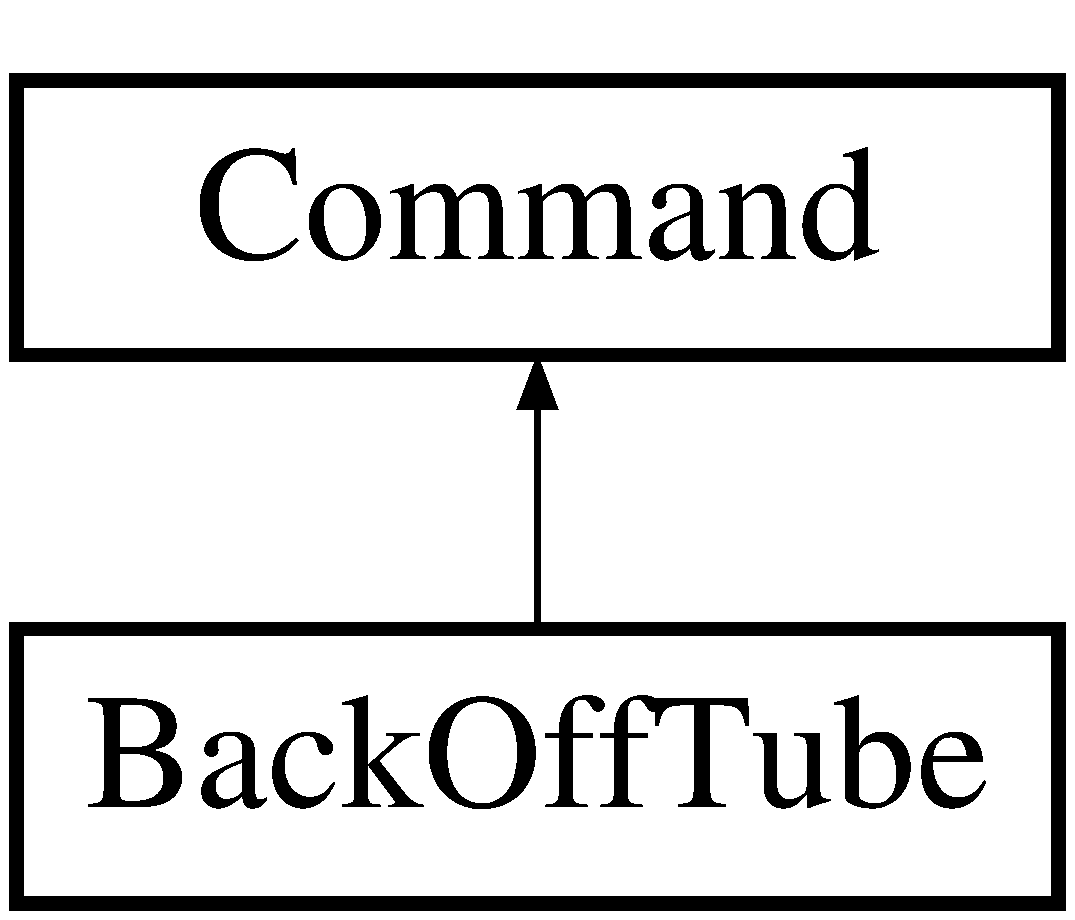
\includegraphics[height=2.000000cm]{classBackOffTube}
\end{center}
\end{figure}
\subsection*{Public Member Functions}
\begin{DoxyCompactItemize}
\item 
\hyperlink{classBackOffTube_ab8fb886043a6df04258ac22415b543dd}{Back\-Off\-Tube} ()
\item 
\hyperlink{classBackOffTube_a6fedeb5bfc92b531a300ce2d95a1a3bb}{Back\-Off\-Tube} (int left\-Speed, int right\-Speed)
\begin{DoxyCompactList}\small\item\em backs up with set motor speeds \end{DoxyCompactList}\item 
void \hyperlink{classBackOffTube_a16b83364009db3cb58ec6c09458a8741}{initialize} ()
\begin{DoxyCompactList}\small\item\em sets a timeout for the time that the robot backs up \end{DoxyCompactList}\item 
void \hyperlink{classBackOffTube_a9d40125cdd95f7ca2db13a5d48e91a93}{execute} ()
\begin{DoxyCompactList}\small\item\em the robot backs up using the parameters it is given \end{DoxyCompactList}\item 
bool \hyperlink{classBackOffTube_abda2334a9432829830a51195a9cce4e6}{is\-Finished} ()
\item 
void \hyperlink{classBackOffTube_a6753fa3b5148d3b8cc06b8e2f7f02be7}{end} ()
\begin{DoxyCompactList}\small\item\em stops the robot \end{DoxyCompactList}\end{DoxyCompactItemize}
\subsection*{Private Attributes}
\begin{DoxyCompactItemize}
\item 
int \hyperlink{classBackOffTube_aa03d7c0535e3d7dd4c45a0453ea9f3aa}{r\-Power}
\begin{DoxyCompactList}\small\item\em variables used for the command \end{DoxyCompactList}\item 
int \hyperlink{classBackOffTube_a5eee02bb4a6756ea44206e411211aea8}{l\-Power}
\item 
const int \hyperlink{classBackOffTube_a46fdecac50000c6b1e9ecae3e42ea4b4}{back\-Off\-Time} = 550
\begin{DoxyCompactList}\small\item\em the time the robot drives back for \end{DoxyCompactList}\end{DoxyCompactItemize}
\subsection*{Additional Inherited Members}


\subsection{Detailed Description}
backs off of the tube 

Definition at line 8 of file Back\-Off\-Tube.\-h.



\subsection{Constructor \& Destructor Documentation}
\hypertarget{classBackOffTube_ab8fb886043a6df04258ac22415b543dd}{\index{Back\-Off\-Tube@{Back\-Off\-Tube}!Back\-Off\-Tube@{Back\-Off\-Tube}}
\index{Back\-Off\-Tube@{Back\-Off\-Tube}!BackOffTube@{Back\-Off\-Tube}}
\subsubsection[{Back\-Off\-Tube}]{\setlength{\rightskip}{0pt plus 5cm}Back\-Off\-Tube\-::\-Back\-Off\-Tube (
\begin{DoxyParamCaption}
{}
\end{DoxyParamCaption}
)}}\label{classBackOffTube_ab8fb886043a6df04258ac22415b543dd}
\hypertarget{classBackOffTube_a6fedeb5bfc92b531a300ce2d95a1a3bb}{\index{Back\-Off\-Tube@{Back\-Off\-Tube}!Back\-Off\-Tube@{Back\-Off\-Tube}}
\index{Back\-Off\-Tube@{Back\-Off\-Tube}!BackOffTube@{Back\-Off\-Tube}}
\subsubsection[{Back\-Off\-Tube}]{\setlength{\rightskip}{0pt plus 5cm}Back\-Off\-Tube\-::\-Back\-Off\-Tube (
\begin{DoxyParamCaption}
\item[{int}]{left\-Speed, }
\item[{int}]{right\-Speed}
\end{DoxyParamCaption}
)}}\label{classBackOffTube_a6fedeb5bfc92b531a300ce2d95a1a3bb}


backs up with set motor speeds 


\begin{DoxyParams}{Parameters}
{\em leftspeed} & is left motor speed \\
\hline
{\em rightspeed} & is right motor speed \\
\hline
\end{DoxyParams}


Definition at line 3 of file Back\-Off\-Tube.\-cpp.



\subsection{Member Function Documentation}
\hypertarget{classBackOffTube_a6753fa3b5148d3b8cc06b8e2f7f02be7}{\index{Back\-Off\-Tube@{Back\-Off\-Tube}!end@{end}}
\index{end@{end}!BackOffTube@{Back\-Off\-Tube}}
\subsubsection[{end}]{\setlength{\rightskip}{0pt plus 5cm}void Back\-Off\-Tube\-::end (
\begin{DoxyParamCaption}
{}
\end{DoxyParamCaption}
)\hspace{0.3cm}{\ttfamily [virtual]}}}\label{classBackOffTube_a6753fa3b5148d3b8cc06b8e2f7f02be7}


stops the robot 



Reimplemented from \hyperlink{classCommand_a147da4a43c939870018324a0af4c7b0b}{Command}.



Definition at line 20 of file Back\-Off\-Tube.\-cpp.

\hypertarget{classBackOffTube_a9d40125cdd95f7ca2db13a5d48e91a93}{\index{Back\-Off\-Tube@{Back\-Off\-Tube}!execute@{execute}}
\index{execute@{execute}!BackOffTube@{Back\-Off\-Tube}}
\subsubsection[{execute}]{\setlength{\rightskip}{0pt plus 5cm}void Back\-Off\-Tube\-::execute (
\begin{DoxyParamCaption}
{}
\end{DoxyParamCaption}
)\hspace{0.3cm}{\ttfamily [virtual]}}}\label{classBackOffTube_a9d40125cdd95f7ca2db13a5d48e91a93}


the robot backs up using the parameters it is given 



Reimplemented from \hyperlink{classCommand_abc8574913684044b0f1a9f810b4e969b}{Command}.



Definition at line 12 of file Back\-Off\-Tube.\-cpp.

\hypertarget{classBackOffTube_a16b83364009db3cb58ec6c09458a8741}{\index{Back\-Off\-Tube@{Back\-Off\-Tube}!initialize@{initialize}}
\index{initialize@{initialize}!BackOffTube@{Back\-Off\-Tube}}
\subsubsection[{initialize}]{\setlength{\rightskip}{0pt plus 5cm}void Back\-Off\-Tube\-::initialize (
\begin{DoxyParamCaption}
{}
\end{DoxyParamCaption}
)\hspace{0.3cm}{\ttfamily [virtual]}}}\label{classBackOffTube_a16b83364009db3cb58ec6c09458a8741}


sets a timeout for the time that the robot backs up 



Reimplemented from \hyperlink{classCommand_a8044ac332a61df571c3454d9fea9684a}{Command}.



Definition at line 8 of file Back\-Off\-Tube.\-cpp.

\hypertarget{classBackOffTube_abda2334a9432829830a51195a9cce4e6}{\index{Back\-Off\-Tube@{Back\-Off\-Tube}!is\-Finished@{is\-Finished}}
\index{is\-Finished@{is\-Finished}!BackOffTube@{Back\-Off\-Tube}}
\subsubsection[{is\-Finished}]{\setlength{\rightskip}{0pt plus 5cm}bool Back\-Off\-Tube\-::is\-Finished (
\begin{DoxyParamCaption}
{}
\end{DoxyParamCaption}
)\hspace{0.3cm}{\ttfamily [virtual]}}}\label{classBackOffTube_abda2334a9432829830a51195a9cce4e6}
\begin{DoxyReturn}{Returns}
true if timeout has occured 
\end{DoxyReturn}


Reimplemented from \hyperlink{classCommand_ae5846b4332a262e055c7a96759fa18f2}{Command}.



Definition at line 16 of file Back\-Off\-Tube.\-cpp.



\subsection{Member Data Documentation}
\hypertarget{classBackOffTube_a46fdecac50000c6b1e9ecae3e42ea4b4}{\index{Back\-Off\-Tube@{Back\-Off\-Tube}!back\-Off\-Time@{back\-Off\-Time}}
\index{back\-Off\-Time@{back\-Off\-Time}!BackOffTube@{Back\-Off\-Tube}}
\subsubsection[{back\-Off\-Time}]{\setlength{\rightskip}{0pt plus 5cm}const int Back\-Off\-Tube\-::back\-Off\-Time = 550\hspace{0.3cm}{\ttfamily [private]}}}\label{classBackOffTube_a46fdecac50000c6b1e9ecae3e42ea4b4}


the time the robot drives back for 



Definition at line 46 of file Back\-Off\-Tube.\-h.

\hypertarget{classBackOffTube_a5eee02bb4a6756ea44206e411211aea8}{\index{Back\-Off\-Tube@{Back\-Off\-Tube}!l\-Power@{l\-Power}}
\index{l\-Power@{l\-Power}!BackOffTube@{Back\-Off\-Tube}}
\subsubsection[{l\-Power}]{\setlength{\rightskip}{0pt plus 5cm}int Back\-Off\-Tube\-::l\-Power\hspace{0.3cm}{\ttfamily [private]}}}\label{classBackOffTube_a5eee02bb4a6756ea44206e411211aea8}


Definition at line 41 of file Back\-Off\-Tube.\-h.

\hypertarget{classBackOffTube_aa03d7c0535e3d7dd4c45a0453ea9f3aa}{\index{Back\-Off\-Tube@{Back\-Off\-Tube}!r\-Power@{r\-Power}}
\index{r\-Power@{r\-Power}!BackOffTube@{Back\-Off\-Tube}}
\subsubsection[{r\-Power}]{\setlength{\rightskip}{0pt plus 5cm}int Back\-Off\-Tube\-::r\-Power\hspace{0.3cm}{\ttfamily [private]}}}\label{classBackOffTube_aa03d7c0535e3d7dd4c45a0453ea9f3aa}


variables used for the command 



Definition at line 41 of file Back\-Off\-Tube.\-h.



The documentation for this class was generated from the following files\-:\begin{DoxyCompactItemize}
\item 
Final\-\_\-\-Project/\hyperlink{BackOffTube_8h}{Back\-Off\-Tube.\-h}\item 
Final\-\_\-\-Project/\hyperlink{BackOffTube_8cpp}{Back\-Off\-Tube.\-cpp}\end{DoxyCompactItemize}

\hypertarget{classBlinkLED}{\section{Blink\-L\-E\-D Class Reference}
\label{classBlinkLED}\index{Blink\-L\-E\-D@{Blink\-L\-E\-D}}
}
Inheritance diagram for Blink\-L\-E\-D\-:\begin{figure}[H]
\begin{center}
\leavevmode
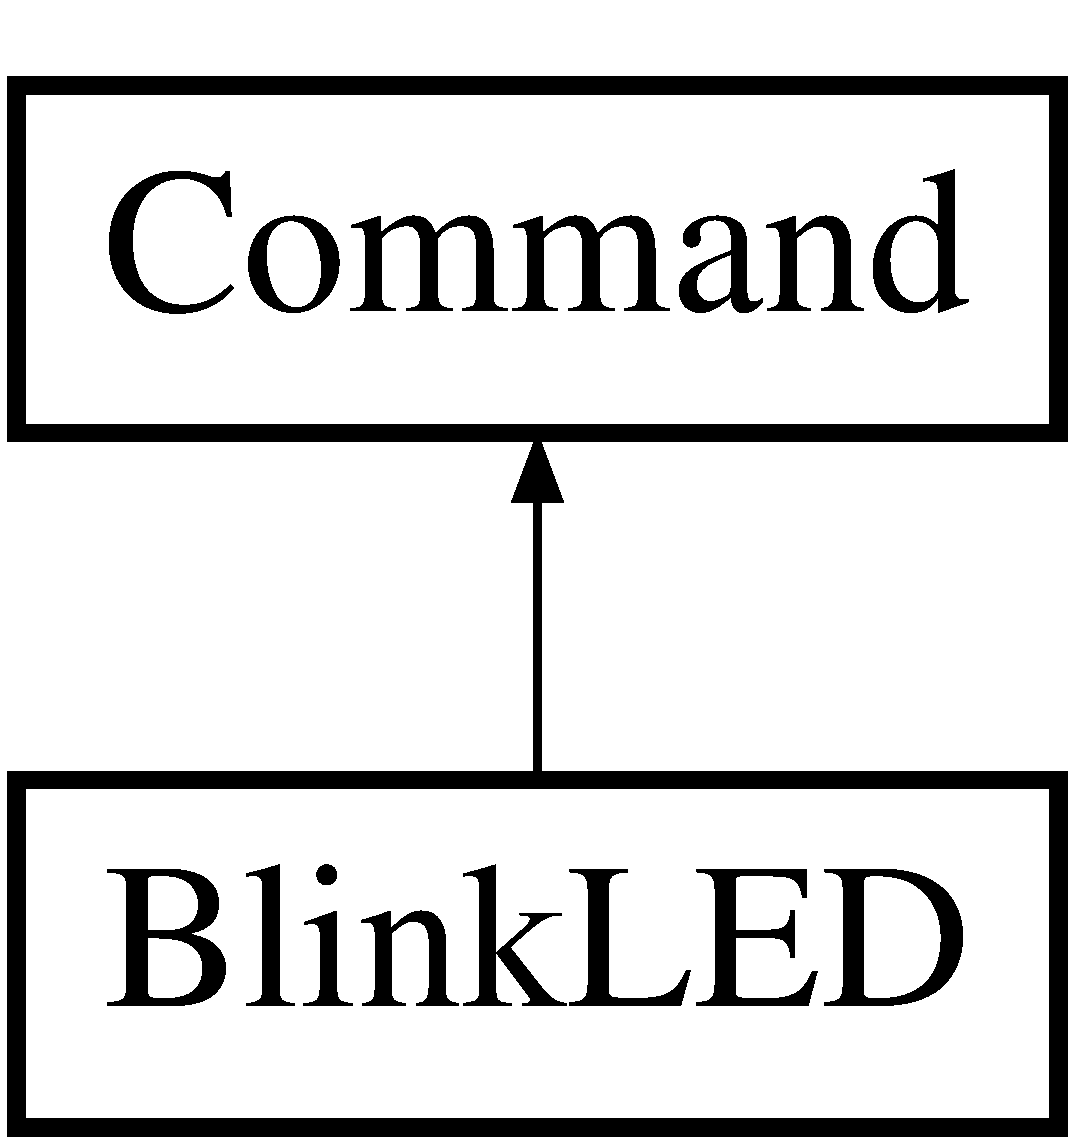
\includegraphics[height=2.000000cm]{classBlinkLED}
\end{center}
\end{figure}
\subsection*{Public Member Functions}
\begin{DoxyCompactItemize}
\item 
\hypertarget{classBlinkLED_adc66eb9bd3f5f7f93eb4e3a534b66d8a}{void \hyperlink{classBlinkLED_adc66eb9bd3f5f7f93eb4e3a534b66d8a}{initialize} ()}\label{classBlinkLED_adc66eb9bd3f5f7f93eb4e3a534b66d8a}

\begin{DoxyCompactList}\small\item\em run once in the first iteration of the command's life. this will be overrided by individual commands \end{DoxyCompactList}\item 
\hypertarget{classBlinkLED_ac7558fcb54cec351245b301d47c0cc87}{void \hyperlink{classBlinkLED_ac7558fcb54cec351245b301d47c0cc87}{execute} ()}\label{classBlinkLED_ac7558fcb54cec351245b301d47c0cc87}

\begin{DoxyCompactList}\small\item\em stuff to do over and over each iteration. this will be overrided by individual commands \end{DoxyCompactList}\item 
\hypertarget{classBlinkLED_a12866e157f0a19e78dc9169a98774993}{void \hyperlink{classBlinkLED_a12866e157f0a19e78dc9169a98774993}{end} ()}\label{classBlinkLED_a12866e157f0a19e78dc9169a98774993}

\begin{DoxyCompactList}\small\item\em called once at the end, once \hyperlink{classBlinkLED_a44ee1f75ceef08cacdcc9392aa1f81ab}{is\-Finished()} returned true. this will be overrided by individual commands. \end{DoxyCompactList}\item 
bool \hyperlink{classBlinkLED_a44ee1f75ceef08cacdcc9392aa1f81ab}{is\-Finished} ()
\begin{DoxyCompactList}\small\item\em checked every iteration to see if we're done here. this will be overrided by individual commands \end{DoxyCompactList}\end{DoxyCompactItemize}
\subsection*{Additional Inherited Members}


\subsection{Member Function Documentation}
\hypertarget{classBlinkLED_a44ee1f75ceef08cacdcc9392aa1f81ab}{\index{Blink\-L\-E\-D@{Blink\-L\-E\-D}!is\-Finished@{is\-Finished}}
\index{is\-Finished@{is\-Finished}!BlinkLED@{Blink\-L\-E\-D}}
\subsubsection[{is\-Finished}]{\setlength{\rightskip}{0pt plus 5cm}bool Blink\-L\-E\-D\-::is\-Finished (
\begin{DoxyParamCaption}
{}
\end{DoxyParamCaption}
)\hspace{0.3cm}{\ttfamily [virtual]}}}\label{classBlinkLED_a44ee1f75ceef08cacdcc9392aa1f81ab}


checked every iteration to see if we're done here. this will be overrided by individual commands 

\begin{DoxyReturn}{Returns}
is the function finished 
\end{DoxyReturn}


Implements \hyperlink{classCommand_a9aa704d5f9d98f510a79e645701dc72a}{Command}.



The documentation for this class was generated from the following files\-:\begin{DoxyCompactItemize}
\item 
Final\-\_\-\-Project/Blink\-L\-E\-D.\-h\item 
Final\-\_\-\-Project/Blink\-L\-E\-D.\-cpp\end{DoxyCompactItemize}

\hypertarget{classBTClient}{\section{B\-T\-Client Class Reference}
\label{classBTClient}\index{B\-T\-Client@{B\-T\-Client}}
}
\subsection*{Public Member Functions}
\begin{DoxyCompactItemize}
\item 
\hypertarget{classBTClient_aefdc156fe1f22455d249ec0bb7fa3fd5}{void {\bfseries setup} ()}\label{classBTClient_aefdc156fe1f22455d249ec0bb7fa3fd5}

\item 
\hypertarget{classBTClient_a8305c35eac468b66f6e8cfe18b331e04}{byte {\bfseries available\-Supply\-Tubes} ()}\label{classBTClient_a8305c35eac468b66f6e8cfe18b331e04}

\item 
\hypertarget{classBTClient_a4c0882cd410b694e9f9406c6e2c58dc8}{byte {\bfseries open\-Storage\-Tubes} ()}\label{classBTClient_a4c0882cd410b694e9f9406c6e2c58dc8}

\item 
\hypertarget{classBTClient_a70cc30b8de8632bd6fb81972a9409a10}{void {\bfseries send\-Radiation\-Alert} ()}\label{classBTClient_a70cc30b8de8632bd6fb81972a9409a10}

\item 
\hypertarget{classBTClient_a4bf8f58f2c83834cab585e69c55c171f}{void {\bfseries send\-Heartbeat} ()}\label{classBTClient_a4bf8f58f2c83834cab585e69c55c171f}

\item 
\hypertarget{classBTClient_a57a82b64a1233a66450c1d9ebe48774c}{void {\bfseries send\-Debug\-String} (String message)}\label{classBTClient_a57a82b64a1233a66450c1d9ebe48774c}

\item 
\hypertarget{classBTClient_a8e827d16926d45a4b7c18dda0e59837b}{void {\bfseries read\-Message} ()}\label{classBTClient_a8e827d16926d45a4b7c18dda0e59837b}

\end{DoxyCompactItemize}


The documentation for this class was generated from the following files\-:\begin{DoxyCompactItemize}
\item 
Final\-\_\-\-Project/B\-T\-Client.\-h\item 
Final\-\_\-\-Project/B\-T\-Client.\-cpp\end{DoxyCompactItemize}

\hypertarget{classCalibrate}{\section{Calibrate Class Reference}
\label{classCalibrate}\index{Calibrate@{Calibrate}}
}


{\ttfamily \#include $<$Calibrate.\-h$>$}

Inheritance diagram for Calibrate\-:\begin{figure}[H]
\begin{center}
\leavevmode
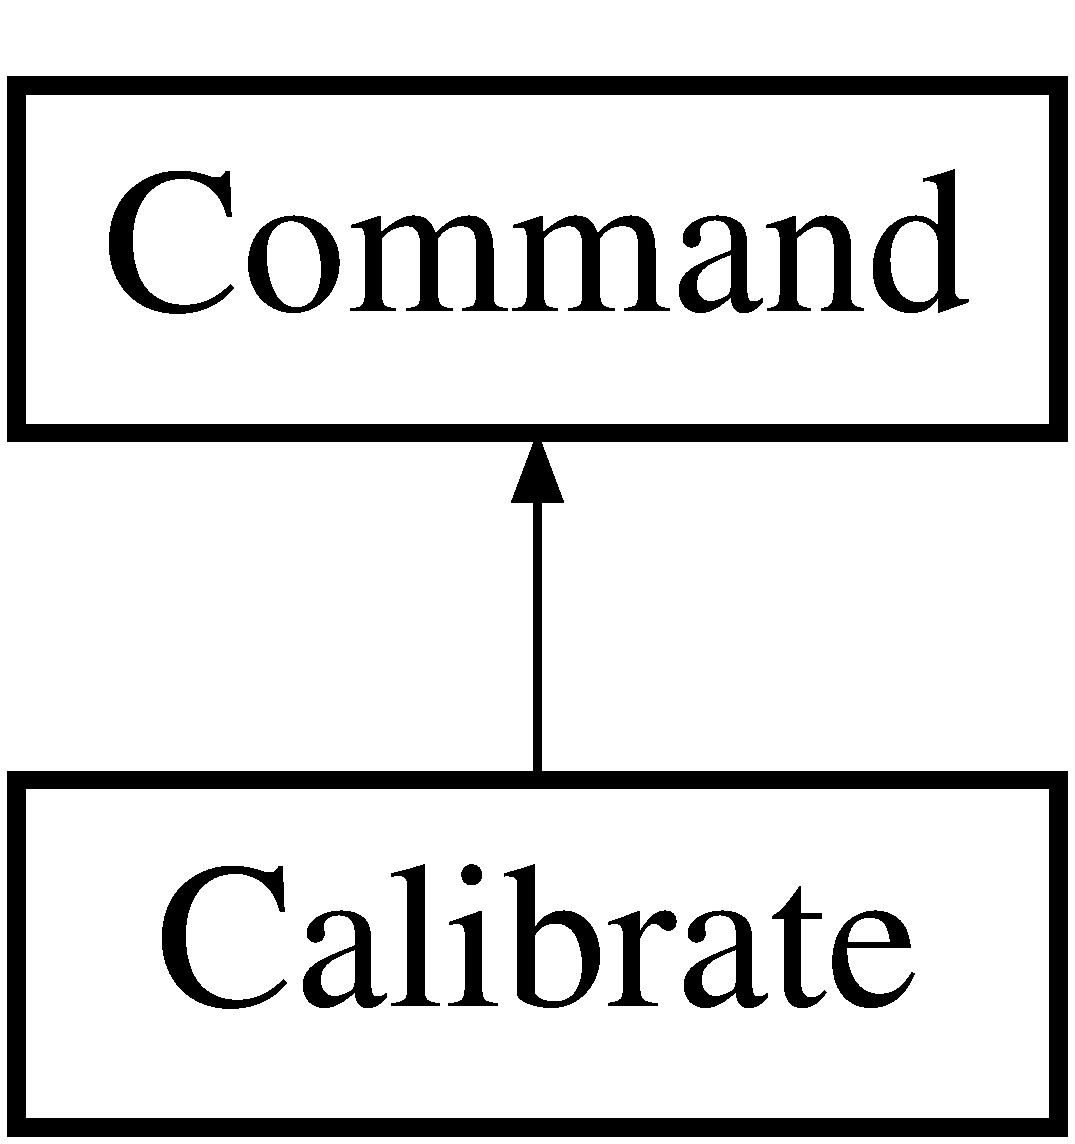
\includegraphics[height=2.000000cm]{classCalibrate}
\end{center}
\end{figure}
\subsection*{Public Member Functions}
\begin{DoxyCompactItemize}
\item 
\hyperlink{classCalibrate_af7fd8ee2339ee66f6f8e4d9953025796}{Calibrate} ()
\item 
void \hyperlink{classCalibrate_a67ac70871401c5b6e74fa92fa4b57f1e}{initialize} ()
\begin{DoxyCompactList}\small\item\em run once in the first iteration of the command's life. this will be overrided by individual commands \end{DoxyCompactList}\item 
void \hyperlink{classCalibrate_ac4d34bf2f831065219b7a930b0389b6e}{execute} ()
\begin{DoxyCompactList}\small\item\em stuff to do over and over each iteration. this will be overrided by individual commands \end{DoxyCompactList}\item 
bool \hyperlink{classCalibrate_afb77ae82fa06d139612f11dec7b6ed5f}{is\-Finished} ()
\begin{DoxyCompactList}\small\item\em checked every iteration to see if we're done here. this will be overrided by individual commands \end{DoxyCompactList}\item 
void \hyperlink{classCalibrate_a2ea8ff643d8450473d6245e407415f03}{end} ()
\begin{DoxyCompactList}\small\item\em called once at the end, once \hyperlink{classCalibrate_afb77ae82fa06d139612f11dec7b6ed5f}{is\-Finished()} returned true. this will be overrided by individual commands. \end{DoxyCompactList}\end{DoxyCompactItemize}
\subsection*{Private Attributes}
\begin{DoxyCompactItemize}
\item 
int \hyperlink{classCalibrate_a76f63e45bd236101217c023f5b4c00d0}{min\-Val}
\item 
int \hyperlink{classCalibrate_a48cdb0fd93fef77a7eab3fc629e9d2a6}{max\-Val}
\end{DoxyCompactItemize}
\subsection*{Additional Inherited Members}


\subsection{Detailed Description}


Definition at line 6 of file Calibrate.\-h.



\subsection{Constructor \& Destructor Documentation}
\hypertarget{classCalibrate_af7fd8ee2339ee66f6f8e4d9953025796}{\index{Calibrate@{Calibrate}!Calibrate@{Calibrate}}
\index{Calibrate@{Calibrate}!Calibrate@{Calibrate}}
\subsubsection[{Calibrate}]{\setlength{\rightskip}{0pt plus 5cm}Calibrate\-::\-Calibrate (
\begin{DoxyParamCaption}
{}
\end{DoxyParamCaption}
)}}\label{classCalibrate_af7fd8ee2339ee66f6f8e4d9953025796}


\subsection{Member Function Documentation}
\hypertarget{classCalibrate_a2ea8ff643d8450473d6245e407415f03}{\index{Calibrate@{Calibrate}!end@{end}}
\index{end@{end}!Calibrate@{Calibrate}}
\subsubsection[{end}]{\setlength{\rightskip}{0pt plus 5cm}void Calibrate\-::end (
\begin{DoxyParamCaption}
{}
\end{DoxyParamCaption}
)\hspace{0.3cm}{\ttfamily [virtual]}}}\label{classCalibrate_a2ea8ff643d8450473d6245e407415f03}


called once at the end, once \hyperlink{classCalibrate_afb77ae82fa06d139612f11dec7b6ed5f}{is\-Finished()} returned true. this will be overrided by individual commands. 



Implements \hyperlink{classCommand_abed8b7871ba1078bc10056cac5b471be}{Command}.

\hypertarget{classCalibrate_ac4d34bf2f831065219b7a930b0389b6e}{\index{Calibrate@{Calibrate}!execute@{execute}}
\index{execute@{execute}!Calibrate@{Calibrate}}
\subsubsection[{execute}]{\setlength{\rightskip}{0pt plus 5cm}void Calibrate\-::execute (
\begin{DoxyParamCaption}
{}
\end{DoxyParamCaption}
)\hspace{0.3cm}{\ttfamily [virtual]}}}\label{classCalibrate_ac4d34bf2f831065219b7a930b0389b6e}


stuff to do over and over each iteration. this will be overrided by individual commands 



Implements \hyperlink{classCommand_a6fd7d9bd8df8bfc881e4d6c7cd1878b7}{Command}.

\hypertarget{classCalibrate_a67ac70871401c5b6e74fa92fa4b57f1e}{\index{Calibrate@{Calibrate}!initialize@{initialize}}
\index{initialize@{initialize}!Calibrate@{Calibrate}}
\subsubsection[{initialize}]{\setlength{\rightskip}{0pt plus 5cm}void Calibrate\-::initialize (
\begin{DoxyParamCaption}
{}
\end{DoxyParamCaption}
)\hspace{0.3cm}{\ttfamily [virtual]}}}\label{classCalibrate_a67ac70871401c5b6e74fa92fa4b57f1e}


run once in the first iteration of the command's life. this will be overrided by individual commands 



Implements \hyperlink{classCommand_af186abe582ab15ac64750e4b5d7944de}{Command}.

\hypertarget{classCalibrate_afb77ae82fa06d139612f11dec7b6ed5f}{\index{Calibrate@{Calibrate}!is\-Finished@{is\-Finished}}
\index{is\-Finished@{is\-Finished}!Calibrate@{Calibrate}}
\subsubsection[{is\-Finished}]{\setlength{\rightskip}{0pt plus 5cm}bool Calibrate\-::is\-Finished (
\begin{DoxyParamCaption}
{}
\end{DoxyParamCaption}
)\hspace{0.3cm}{\ttfamily [virtual]}}}\label{classCalibrate_afb77ae82fa06d139612f11dec7b6ed5f}


checked every iteration to see if we're done here. this will be overrided by individual commands 

\begin{DoxyReturn}{Returns}
is the function finished 
\end{DoxyReturn}


Implements \hyperlink{classCommand_a9aa704d5f9d98f510a79e645701dc72a}{Command}.



\subsection{Member Data Documentation}
\hypertarget{classCalibrate_a48cdb0fd93fef77a7eab3fc629e9d2a6}{\index{Calibrate@{Calibrate}!max\-Val@{max\-Val}}
\index{max\-Val@{max\-Val}!Calibrate@{Calibrate}}
\subsubsection[{max\-Val}]{\setlength{\rightskip}{0pt plus 5cm}int Calibrate\-::max\-Val\hspace{0.3cm}{\ttfamily [private]}}}\label{classCalibrate_a48cdb0fd93fef77a7eab3fc629e9d2a6}


Definition at line 14 of file Calibrate.\-h.

\hypertarget{classCalibrate_a76f63e45bd236101217c023f5b4c00d0}{\index{Calibrate@{Calibrate}!min\-Val@{min\-Val}}
\index{min\-Val@{min\-Val}!Calibrate@{Calibrate}}
\subsubsection[{min\-Val}]{\setlength{\rightskip}{0pt plus 5cm}int Calibrate\-::min\-Val\hspace{0.3cm}{\ttfamily [private]}}}\label{classCalibrate_a76f63e45bd236101217c023f5b4c00d0}


Definition at line 14 of file Calibrate.\-h.



The documentation for this class was generated from the following file\-:\begin{DoxyCompactItemize}
\item 
Final\-\_\-\-Project/\hyperlink{Calibrate_8h}{Calibrate.\-h}\end{DoxyCompactItemize}

\hypertarget{classCalibrateRoutine}{\section{Calibrate\-Routine Class Reference}
\label{classCalibrateRoutine}\index{Calibrate\-Routine@{Calibrate\-Routine}}
}


opens the gripper and raises the arm, calibrates line sensor then turns until a line  




{\ttfamily \#include $<$Calibrate\-Routine.\-h$>$}

Inheritance diagram for Calibrate\-Routine\-:\begin{figure}[H]
\begin{center}
\leavevmode
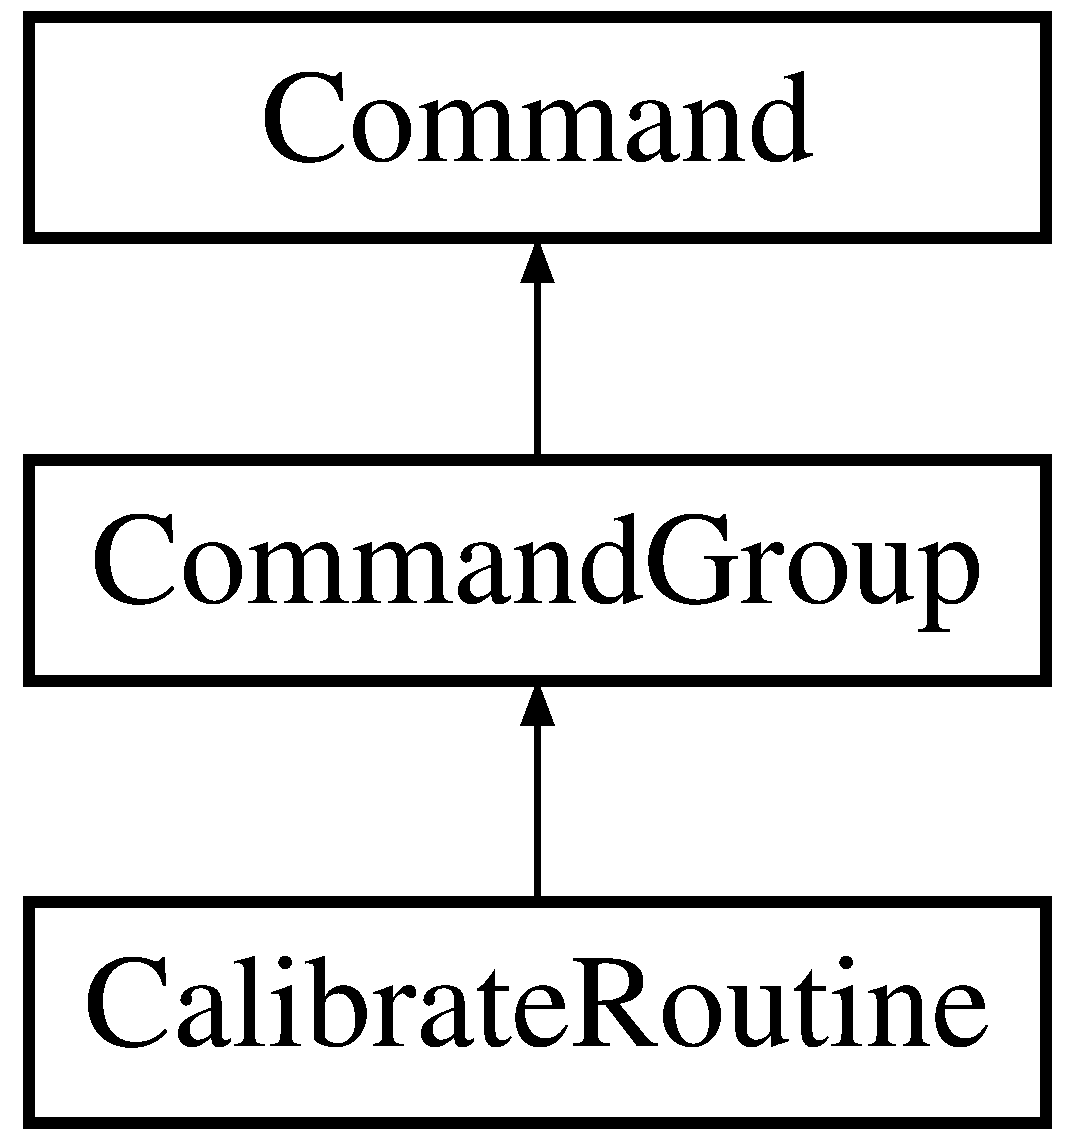
\includegraphics[height=3.000000cm]{classCalibrateRoutine}
\end{center}
\end{figure}
\subsection*{Public Member Functions}
\begin{DoxyCompactItemize}
\item 
\hyperlink{classCalibrateRoutine_ab748a49d319d415cbaa59a192afd4a27}{Calibrate\-Routine} ()
\end{DoxyCompactItemize}
\subsection*{Additional Inherited Members}


\subsection{Detailed Description}
opens the gripper and raises the arm, calibrates line sensor then turns until a line 

Definition at line 7 of file Calibrate\-Routine.\-h.



\subsection{Constructor \& Destructor Documentation}
\hypertarget{classCalibrateRoutine_ab748a49d319d415cbaa59a192afd4a27}{\index{Calibrate\-Routine@{Calibrate\-Routine}!Calibrate\-Routine@{Calibrate\-Routine}}
\index{Calibrate\-Routine@{Calibrate\-Routine}!CalibrateRoutine@{Calibrate\-Routine}}
\subsubsection[{Calibrate\-Routine}]{\setlength{\rightskip}{0pt plus 5cm}Calibrate\-Routine\-::\-Calibrate\-Routine (
\begin{DoxyParamCaption}
{}
\end{DoxyParamCaption}
)}}\label{classCalibrateRoutine_ab748a49d319d415cbaa59a192afd4a27}


Definition at line 9 of file Calibrate\-Routine.\-cpp.



The documentation for this class was generated from the following files\-:\begin{DoxyCompactItemize}
\item 
Final\-\_\-\-Project/\hyperlink{CalibrateRoutine_8h}{Calibrate\-Routine.\-h}\item 
Final\-\_\-\-Project/\hyperlink{CalibrateRoutine_8cpp}{Calibrate\-Routine.\-cpp}\end{DoxyCompactItemize}

\hypertarget{classCloseGripper}{\section{Close\-Gripper Class Reference}
\label{classCloseGripper}\index{Close\-Gripper@{Close\-Gripper}}
}


closes the gripper  




{\ttfamily \#include $<$Close\-Gripper.\-h$>$}

Inheritance diagram for Close\-Gripper\-:\begin{figure}[H]
\begin{center}
\leavevmode
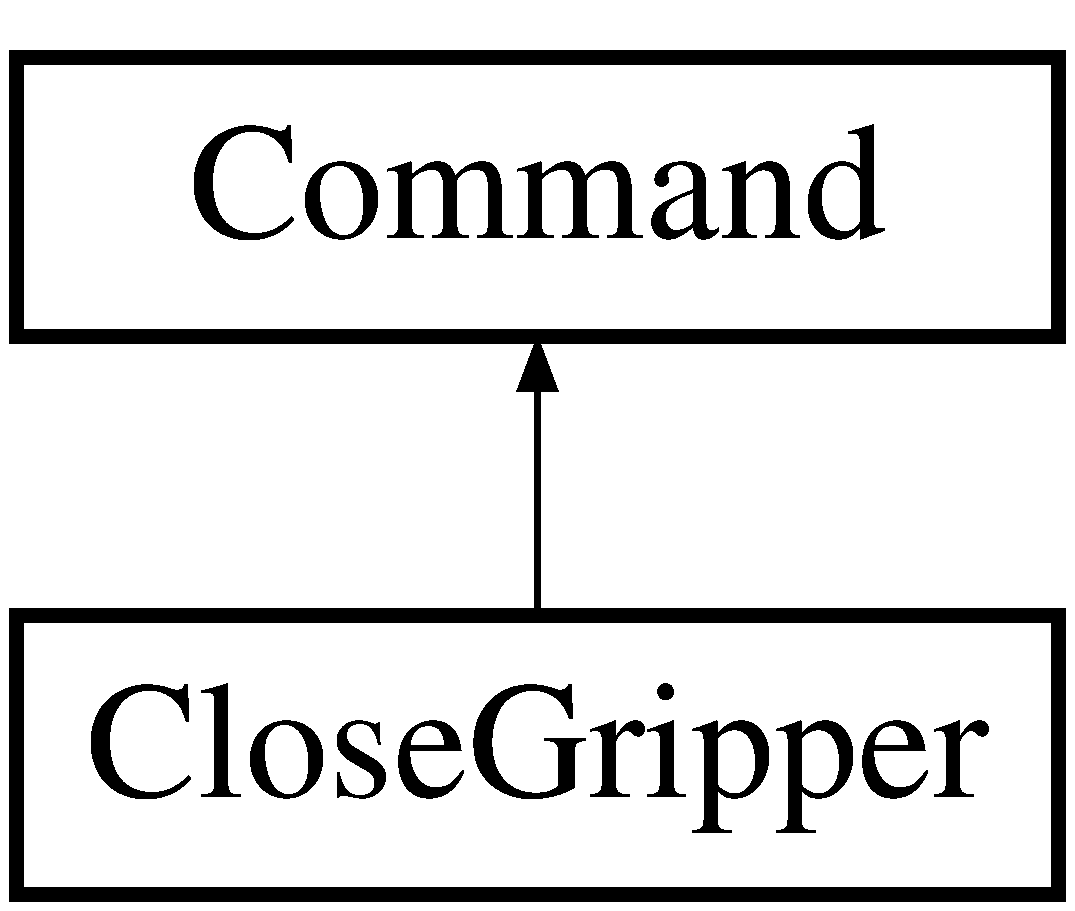
\includegraphics[height=2.000000cm]{classCloseGripper}
\end{center}
\end{figure}
\subsection*{Public Member Functions}
\begin{DoxyCompactItemize}
\item 
\hyperlink{classCloseGripper_a64f2e7352ab7dfc8217760d8fc882b13}{Close\-Gripper} (int \hyperlink{classCloseGripper_ac90b3c4ad2ba86181bdfa5a3f926593c}{force})
\item 
\hyperlink{classCloseGripper_ac95731a5048d22a12eb77f85fa4f254a}{Close\-Gripper} ()
\item 
void \hyperlink{classCloseGripper_a91b194b7afe5bdc70ccb97fb6a77e956}{initialize} ()
\begin{DoxyCompactList}\small\item\em sets a timeout and begins closing the gripper \end{DoxyCompactList}\item 
void \hyperlink{classCloseGripper_a11b489ca1de2f1be5cb82f47345360d8}{execute} ()
\begin{DoxyCompactList}\small\item\em does nothing \end{DoxyCompactList}\item 
bool \hyperlink{classCloseGripper_afab2b93b62904d6fd70a794a9f954abf}{is\-Finished} ()
\item 
void \hyperlink{classCloseGripper_a06ab30ca6e30278ab74e973e268c5d97}{end} ()
\begin{DoxyCompactList}\small\item\em does nothing \end{DoxyCompactList}\end{DoxyCompactItemize}
\subsection*{Static Public Attributes}
\begin{DoxyCompactItemize}
\item 
static const int \hyperlink{classCloseGripper_af1d1dab59b0bddacb0e82e676e47797a}{H\-A\-R\-D} = 180
\item 
static const int \hyperlink{classCloseGripper_a2b6cac5f41e2d57f180fdcf18aacae45}{S\-O\-F\-T} = 165
\end{DoxyCompactItemize}
\subsection*{Private Attributes}
\begin{DoxyCompactItemize}
\item 
int \hyperlink{classCloseGripper_ac90b3c4ad2ba86181bdfa5a3f926593c}{force}
\end{DoxyCompactItemize}
\subsection*{Additional Inherited Members}


\subsection{Detailed Description}
closes the gripper 

Definition at line 8 of file Close\-Gripper.\-h.



\subsection{Constructor \& Destructor Documentation}
\hypertarget{classCloseGripper_a64f2e7352ab7dfc8217760d8fc882b13}{\index{Close\-Gripper@{Close\-Gripper}!Close\-Gripper@{Close\-Gripper}}
\index{Close\-Gripper@{Close\-Gripper}!CloseGripper@{Close\-Gripper}}
\subsubsection[{Close\-Gripper}]{\setlength{\rightskip}{0pt plus 5cm}Close\-Gripper\-::\-Close\-Gripper (
\begin{DoxyParamCaption}
\item[{int}]{force}
\end{DoxyParamCaption}
)}}\label{classCloseGripper_a64f2e7352ab7dfc8217760d8fc882b13}


Definition at line 5 of file Close\-Gripper.\-cpp.

\hypertarget{classCloseGripper_ac95731a5048d22a12eb77f85fa4f254a}{\index{Close\-Gripper@{Close\-Gripper}!Close\-Gripper@{Close\-Gripper}}
\index{Close\-Gripper@{Close\-Gripper}!CloseGripper@{Close\-Gripper}}
\subsubsection[{Close\-Gripper}]{\setlength{\rightskip}{0pt plus 5cm}Close\-Gripper\-::\-Close\-Gripper (
\begin{DoxyParamCaption}
{}
\end{DoxyParamCaption}
)}}\label{classCloseGripper_ac95731a5048d22a12eb77f85fa4f254a}


Definition at line 3 of file Close\-Gripper.\-cpp.



\subsection{Member Function Documentation}
\hypertarget{classCloseGripper_a06ab30ca6e30278ab74e973e268c5d97}{\index{Close\-Gripper@{Close\-Gripper}!end@{end}}
\index{end@{end}!CloseGripper@{Close\-Gripper}}
\subsubsection[{end}]{\setlength{\rightskip}{0pt plus 5cm}void Close\-Gripper\-::end (
\begin{DoxyParamCaption}
{}
\end{DoxyParamCaption}
)\hspace{0.3cm}{\ttfamily [virtual]}}}\label{classCloseGripper_a06ab30ca6e30278ab74e973e268c5d97}


does nothing 



Reimplemented from \hyperlink{classCommand_a147da4a43c939870018324a0af4c7b0b}{Command}.



Definition at line 25 of file Close\-Gripper.\-cpp.

\hypertarget{classCloseGripper_a11b489ca1de2f1be5cb82f47345360d8}{\index{Close\-Gripper@{Close\-Gripper}!execute@{execute}}
\index{execute@{execute}!CloseGripper@{Close\-Gripper}}
\subsubsection[{execute}]{\setlength{\rightskip}{0pt plus 5cm}void Close\-Gripper\-::execute (
\begin{DoxyParamCaption}
{}
\end{DoxyParamCaption}
)\hspace{0.3cm}{\ttfamily [virtual]}}}\label{classCloseGripper_a11b489ca1de2f1be5cb82f47345360d8}


does nothing 



Reimplemented from \hyperlink{classCommand_abc8574913684044b0f1a9f810b4e969b}{Command}.



Definition at line 16 of file Close\-Gripper.\-cpp.

\hypertarget{classCloseGripper_a91b194b7afe5bdc70ccb97fb6a77e956}{\index{Close\-Gripper@{Close\-Gripper}!initialize@{initialize}}
\index{initialize@{initialize}!CloseGripper@{Close\-Gripper}}
\subsubsection[{initialize}]{\setlength{\rightskip}{0pt plus 5cm}void Close\-Gripper\-::initialize (
\begin{DoxyParamCaption}
{}
\end{DoxyParamCaption}
)\hspace{0.3cm}{\ttfamily [virtual]}}}\label{classCloseGripper_a91b194b7afe5bdc70ccb97fb6a77e956}


sets a timeout and begins closing the gripper 



Reimplemented from \hyperlink{classCommand_a8044ac332a61df571c3454d9fea9684a}{Command}.



Definition at line 10 of file Close\-Gripper.\-cpp.

\hypertarget{classCloseGripper_afab2b93b62904d6fd70a794a9f954abf}{\index{Close\-Gripper@{Close\-Gripper}!is\-Finished@{is\-Finished}}
\index{is\-Finished@{is\-Finished}!CloseGripper@{Close\-Gripper}}
\subsubsection[{is\-Finished}]{\setlength{\rightskip}{0pt plus 5cm}bool Close\-Gripper\-::is\-Finished (
\begin{DoxyParamCaption}
{}
\end{DoxyParamCaption}
)\hspace{0.3cm}{\ttfamily [virtual]}}}\label{classCloseGripper_afab2b93b62904d6fd70a794a9f954abf}
\begin{DoxyReturn}{Returns}
true when timeout has occured 
\end{DoxyReturn}


Reimplemented from \hyperlink{classCommand_ae5846b4332a262e055c7a96759fa18f2}{Command}.



Definition at line 20 of file Close\-Gripper.\-cpp.



\subsection{Member Data Documentation}
\hypertarget{classCloseGripper_ac90b3c4ad2ba86181bdfa5a3f926593c}{\index{Close\-Gripper@{Close\-Gripper}!force@{force}}
\index{force@{force}!CloseGripper@{Close\-Gripper}}
\subsubsection[{force}]{\setlength{\rightskip}{0pt plus 5cm}int Close\-Gripper\-::force\hspace{0.3cm}{\ttfamily [private]}}}\label{classCloseGripper_ac90b3c4ad2ba86181bdfa5a3f926593c}


Definition at line 34 of file Close\-Gripper.\-h.

\hypertarget{classCloseGripper_af1d1dab59b0bddacb0e82e676e47797a}{\index{Close\-Gripper@{Close\-Gripper}!H\-A\-R\-D@{H\-A\-R\-D}}
\index{H\-A\-R\-D@{H\-A\-R\-D}!CloseGripper@{Close\-Gripper}}
\subsubsection[{H\-A\-R\-D}]{\setlength{\rightskip}{0pt plus 5cm}const int Close\-Gripper\-::\-H\-A\-R\-D = 180\hspace{0.3cm}{\ttfamily [static]}}}\label{classCloseGripper_af1d1dab59b0bddacb0e82e676e47797a}


Definition at line 31 of file Close\-Gripper.\-h.

\hypertarget{classCloseGripper_a2b6cac5f41e2d57f180fdcf18aacae45}{\index{Close\-Gripper@{Close\-Gripper}!S\-O\-F\-T@{S\-O\-F\-T}}
\index{S\-O\-F\-T@{S\-O\-F\-T}!CloseGripper@{Close\-Gripper}}
\subsubsection[{S\-O\-F\-T}]{\setlength{\rightskip}{0pt plus 5cm}const int Close\-Gripper\-::\-S\-O\-F\-T = 165\hspace{0.3cm}{\ttfamily [static]}}}\label{classCloseGripper_a2b6cac5f41e2d57f180fdcf18aacae45}


Definition at line 32 of file Close\-Gripper.\-h.



The documentation for this class was generated from the following files\-:\begin{DoxyCompactItemize}
\item 
Final\-\_\-\-Project/\hyperlink{CloseGripper_8h}{Close\-Gripper.\-h}\item 
Final\-\_\-\-Project/\hyperlink{CloseGripper_8cpp}{Close\-Gripper.\-cpp}\end{DoxyCompactItemize}

\hypertarget{classCommand}{\section{Command Class Reference}
\label{classCommand}\index{Command@{Command}}
}


this class is the very core of the framework commands are initialized once, then run until they're done completed commands are removed the scheduler  




{\ttfamily \#include $<$Command.\-h$>$}

Inheritance diagram for Command\-:\begin{figure}[H]
\begin{center}
\leavevmode
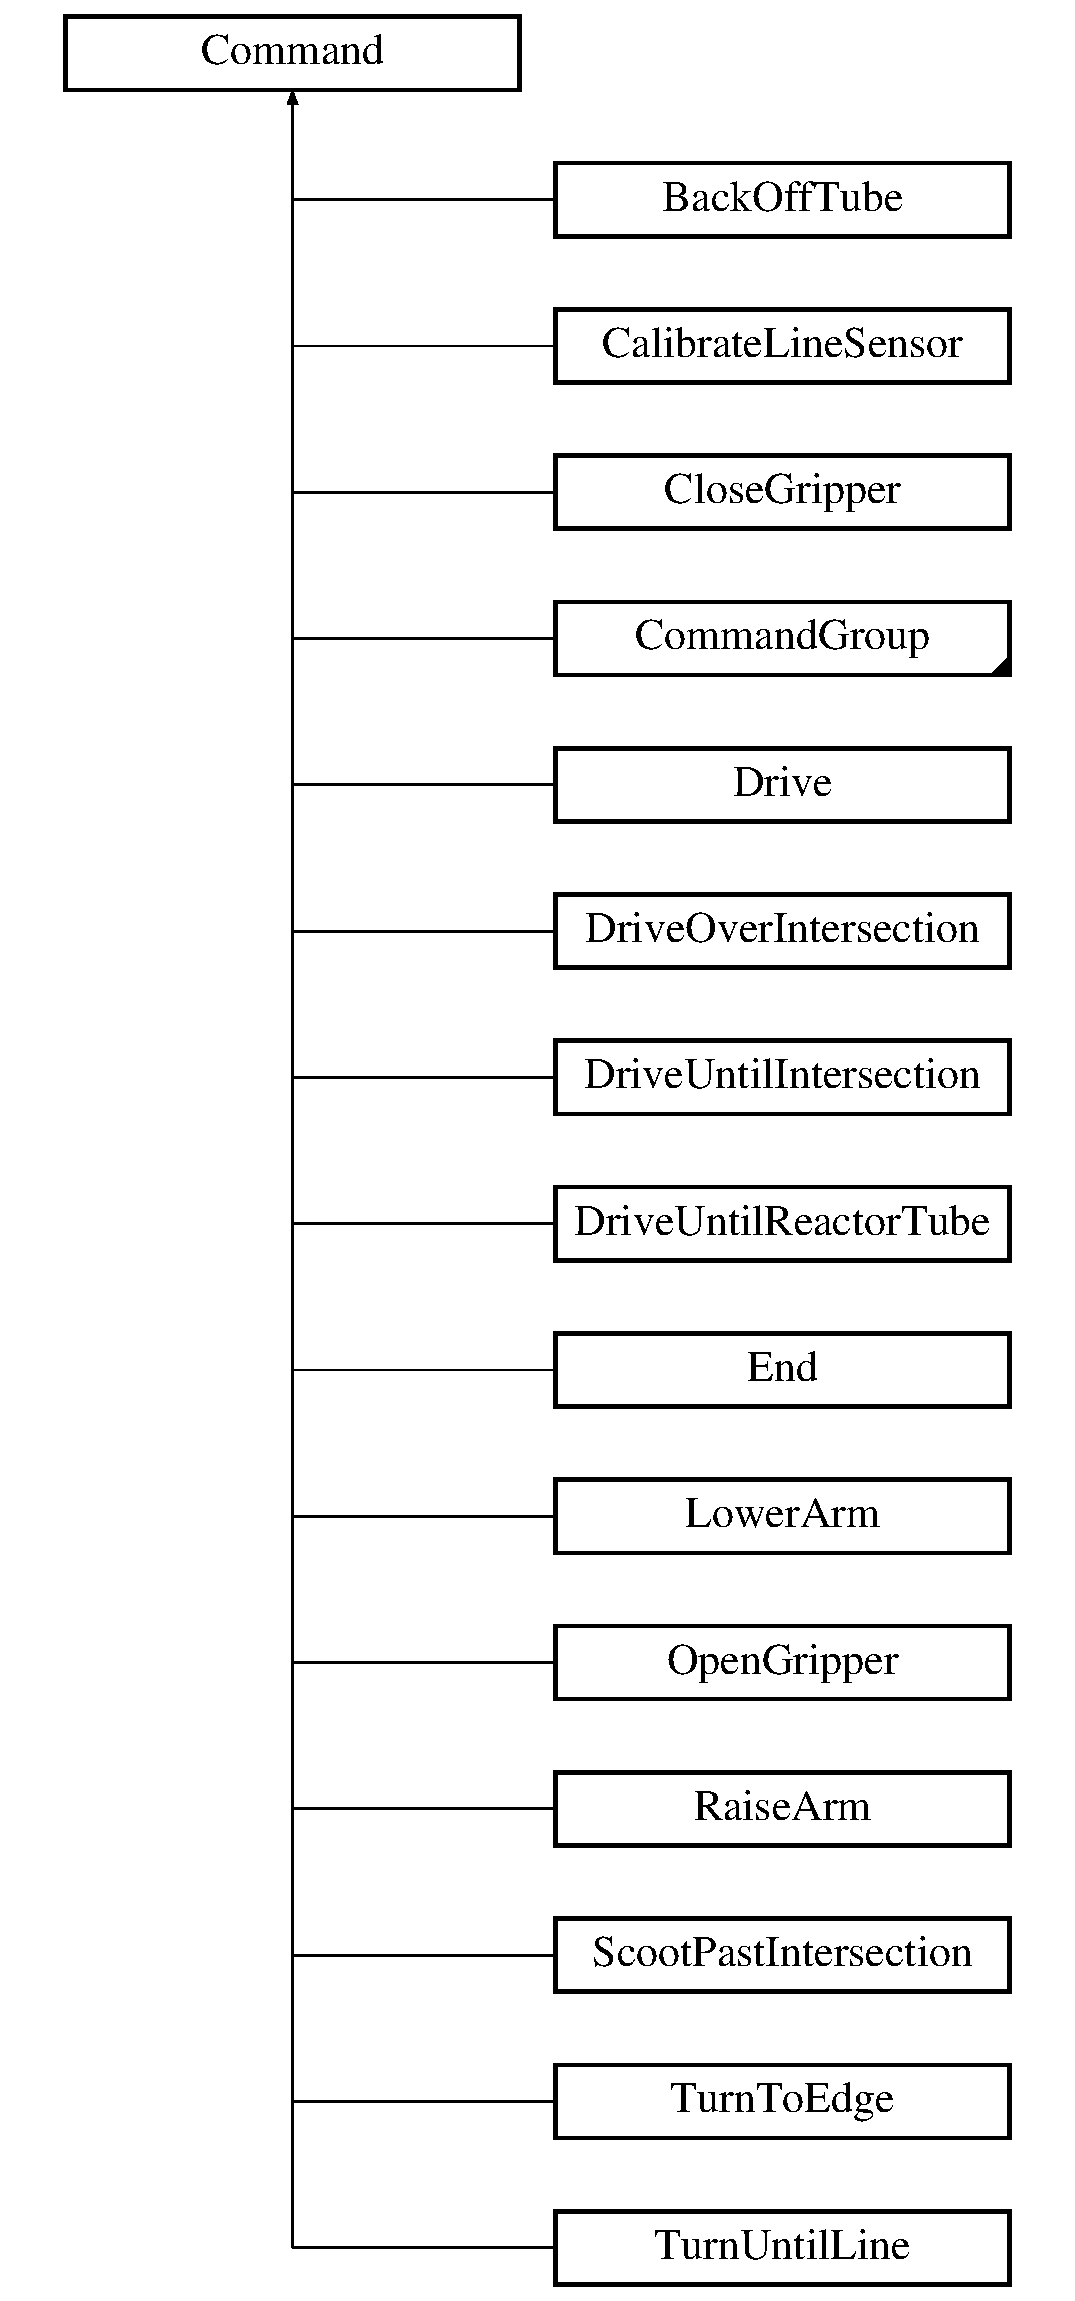
\includegraphics[height=12.000000cm]{classCommand}
\end{center}
\end{figure}
\subsection*{Public Member Functions}
\begin{DoxyCompactItemize}
\item 
\hyperlink{classCommand_a18df2d81039392daeb0b78c346a70537}{Command} ()
\item 
\hyperlink{classCommand_a5f939f31974c4955c486b18a07675698}{Command} (const String \hyperlink{classCommand_a19f7ad73ca8599ad47f9b7bcccc52610}{name})
\item 
void \hyperlink{classCommand_adfbbaa47b15c80c2a713d24e48b843a8}{set\-Timeout} (unsigned long \hyperlink{classCommand_a687b30a3d41c93f91dfba5a88c98f270}{timeout})
\item 
unsigned long \hyperlink{classCommand_a53de8c6445ccd2f51fe7535a71e20c98}{get\-Time} ()
\item 
bool \hyperlink{classCommand_ac62a4b3acc8db6c5e396d5c97ca51a98}{is\-Timed\-Out} ()
\item 
virtual void \hyperlink{classCommand_a8044ac332a61df571c3454d9fea9684a}{initialize} ()
\begin{DoxyCompactList}\small\item\em run once in the first iteration of the command's life. this will be overrided by individual commands \end{DoxyCompactList}\item 
virtual void \hyperlink{classCommand_ae7c58ad4895c51ff18f1d432dbd4f4ec}{\-\_\-initialize} ()
\item 
virtual void \hyperlink{classCommand_abc8574913684044b0f1a9f810b4e969b}{execute} ()
\begin{DoxyCompactList}\small\item\em stuff to do over and over each iteration. this will be overrided by individual commands \end{DoxyCompactList}\item 
virtual void \hyperlink{classCommand_a49e6861e0c14411d6860f0b3211db9c9}{\-\_\-execute} ()
\item 
virtual bool \hyperlink{classCommand_ae5846b4332a262e055c7a96759fa18f2}{is\-Finished} ()
\begin{DoxyCompactList}\small\item\em checked every iteration to see if we're done here. this will be overrided by individual commands \end{DoxyCompactList}\item 
virtual void \hyperlink{classCommand_a147da4a43c939870018324a0af4c7b0b}{end} ()
\begin{DoxyCompactList}\small\item\em called once at the end, once \hyperlink{classCommand_ae5846b4332a262e055c7a96759fa18f2}{is\-Finished()} returned true. this will be overrided by individual commands. \end{DoxyCompactList}\item 
virtual void \hyperlink{classCommand_a9173c74652cb69c8807170bf16151ae2}{\-\_\-end} ()
\item 
void \hyperlink{classCommand_aef139180669b92534dd05a89323fb82f}{start} ()
\begin{DoxyCompactList}\small\item\em adds this command to the scheduler \end{DoxyCompactList}\item 
bool \hyperlink{classCommand_a93e75689d86c0a8675c1f769f721d646}{cycle} ()
\begin{DoxyCompactList}\small\item\em actually does the excuting. \end{DoxyCompactList}\item 
bool \hyperlink{classCommand_a0252c920dd7114c29ef04526cfd0f39a}{is\-Running} ()
\begin{DoxyCompactList}\small\item\em check if the command is running. not yet implemented. \end{DoxyCompactList}\item 
bool \hyperlink{classCommand_a51103f3b209bdbd421f40a38521a9e5e}{operator!=} (const \hyperlink{classCommand}{Command} \&other)
\begin{DoxyCompactList}\small\item\em comparator overload for !=. used when checking if command is in list \end{DoxyCompactList}\item 
void \hyperlink{classCommand_a03a7f03b29c4cbb748a15c9c83233023}{print} ()
\end{DoxyCompactItemize}
\subsection*{Public Attributes}
\begin{DoxyCompactItemize}
\item 
bool \hyperlink{classCommand_ad6e763c58ca2751de879c6eb3f3ae48f}{in\-Parallel}
\begin{DoxyCompactList}\small\item\em used by command group to organize commands \end{DoxyCompactList}\item 
String \hyperlink{classCommand_a19f7ad73ca8599ad47f9b7bcccc52610}{name}
\begin{DoxyCompactList}\small\item\em for convenient printing \end{DoxyCompactList}\end{DoxyCompactItemize}
\subsection*{Private Attributes}
\begin{DoxyCompactItemize}
\item 
bool \hyperlink{classCommand_aa9dd747d430f9367da9b17545404f79e}{initialized}
\item 
bool \hyperlink{classCommand_a8e31897f049af332a2421c9721fda18b}{running}
\item 
unsigned long \hyperlink{classCommand_a687b30a3d41c93f91dfba5a88c98f270}{timeout} = 0
\item 
unsigned long \hyperlink{classCommand_af537856a06286a62d7200d84f901c72e}{start\-Time} = 0
\end{DoxyCompactItemize}


\subsection{Detailed Description}
this class is the very core of the framework commands are initialized once, then run until they're done completed commands are removed the scheduler 

Definition at line 10 of file Command.\-h.



\subsection{Constructor \& Destructor Documentation}
\hypertarget{classCommand_a18df2d81039392daeb0b78c346a70537}{\index{Command@{Command}!Command@{Command}}
\index{Command@{Command}!Command@{Command}}
\subsubsection[{Command}]{\setlength{\rightskip}{0pt plus 5cm}Command\-::\-Command (
\begin{DoxyParamCaption}
{}
\end{DoxyParamCaption}
)}}\label{classCommand_a18df2d81039392daeb0b78c346a70537}


Definition at line 6 of file Command.\-cpp.

\hypertarget{classCommand_a5f939f31974c4955c486b18a07675698}{\index{Command@{Command}!Command@{Command}}
\index{Command@{Command}!Command@{Command}}
\subsubsection[{Command}]{\setlength{\rightskip}{0pt plus 5cm}Command\-::\-Command (
\begin{DoxyParamCaption}
\item[{const String}]{name}
\end{DoxyParamCaption}
)}}\label{classCommand_a5f939f31974c4955c486b18a07675698}


Definition at line 8 of file Command.\-cpp.



\subsection{Member Function Documentation}
\hypertarget{classCommand_a9173c74652cb69c8807170bf16151ae2}{\index{Command@{Command}!\-\_\-end@{\-\_\-end}}
\index{\-\_\-end@{\-\_\-end}!Command@{Command}}
\subsubsection[{\-\_\-end}]{\setlength{\rightskip}{0pt plus 5cm}void Command\-::\-\_\-end (
\begin{DoxyParamCaption}
{}
\end{DoxyParamCaption}
)\hspace{0.3cm}{\ttfamily [virtual]}}}\label{classCommand_a9173c74652cb69c8807170bf16151ae2}


Reimplemented in \hyperlink{classCommandGroup_a11f0ae6eb2ba052138d5a8930f23bb4f}{Command\-Group}.



Definition at line 60 of file Command.\-cpp.

\hypertarget{classCommand_a49e6861e0c14411d6860f0b3211db9c9}{\index{Command@{Command}!\-\_\-execute@{\-\_\-execute}}
\index{\-\_\-execute@{\-\_\-execute}!Command@{Command}}
\subsubsection[{\-\_\-execute}]{\setlength{\rightskip}{0pt plus 5cm}void Command\-::\-\_\-execute (
\begin{DoxyParamCaption}
{}
\end{DoxyParamCaption}
)\hspace{0.3cm}{\ttfamily [virtual]}}}\label{classCommand_a49e6861e0c14411d6860f0b3211db9c9}


Reimplemented in \hyperlink{classCommandGroup_a09355b6bb1018bdadaa0f5a1c0dec007}{Command\-Group}.



Definition at line 55 of file Command.\-cpp.

\hypertarget{classCommand_ae7c58ad4895c51ff18f1d432dbd4f4ec}{\index{Command@{Command}!\-\_\-initialize@{\-\_\-initialize}}
\index{\-\_\-initialize@{\-\_\-initialize}!Command@{Command}}
\subsubsection[{\-\_\-initialize}]{\setlength{\rightskip}{0pt plus 5cm}void Command\-::\-\_\-initialize (
\begin{DoxyParamCaption}
{}
\end{DoxyParamCaption}
)\hspace{0.3cm}{\ttfamily [virtual]}}}\label{classCommand_ae7c58ad4895c51ff18f1d432dbd4f4ec}


Reimplemented in \hyperlink{classCommandGroup_aad0c9576993f9f8d2431cd44f0bf0072}{Command\-Group}.



Definition at line 49 of file Command.\-cpp.

\hypertarget{classCommand_a93e75689d86c0a8675c1f769f721d646}{\index{Command@{Command}!cycle@{cycle}}
\index{cycle@{cycle}!Command@{Command}}
\subsubsection[{cycle}]{\setlength{\rightskip}{0pt plus 5cm}bool Command\-::cycle (
\begin{DoxyParamCaption}
{}
\end{DoxyParamCaption}
)}}\label{classCommand_a93e75689d86c0a8675c1f769f721d646}


actually does the excuting. 

\begin{DoxyReturn}{Returns}
if command is finished 
\end{DoxyReturn}


Definition at line 10 of file Command.\-cpp.

\hypertarget{classCommand_a147da4a43c939870018324a0af4c7b0b}{\index{Command@{Command}!end@{end}}
\index{end@{end}!Command@{Command}}
\subsubsection[{end}]{\setlength{\rightskip}{0pt plus 5cm}void Command\-::end (
\begin{DoxyParamCaption}
{}
\end{DoxyParamCaption}
)\hspace{0.3cm}{\ttfamily [virtual]}}}\label{classCommand_a147da4a43c939870018324a0af4c7b0b}


called once at the end, once \hyperlink{classCommand_ae5846b4332a262e055c7a96759fa18f2}{is\-Finished()} returned true. this will be overrided by individual commands. 



Reimplemented in \hyperlink{classBackOffTube_a6753fa3b5148d3b8cc06b8e2f7f02be7}{Back\-Off\-Tube}, \hyperlink{classTurnUntilLine_a769864873e706e0ca6701eac7f947ede}{Turn\-Until\-Line}, \hyperlink{classTurnOffLine_ad888d865fb75e8139825f4dcf7709f1e}{Turn\-Off\-Line}, \hyperlink{classCloseGripper_a06ab30ca6e30278ab74e973e268c5d97}{Close\-Gripper}, \hyperlink{classDriveUntilReactorTube_a34011a5721faf7cd169ac4e56f9c901b}{Drive\-Until\-Reactor\-Tube}, \hyperlink{classCalibrateLineSensor_ae5cdfbb59fa0fd63828ae70f865998b2}{Calibrate\-Line\-Sensor}, \hyperlink{classDrive_aa52dc86430f29f4ddc7c6b7c35bd2232}{Drive}, \hyperlink{classDriveOverIntersection_a90d8b3592d6c67e9ef1ae1a6396aa1c2}{Drive\-Over\-Intersection}, \hyperlink{classDriveUntilIntersection_a309d1f37d92844707c2f3dcb2f5d5638}{Drive\-Until\-Intersection}, \hyperlink{classLowerArm_aa46179794b13132a2a353f24c785db37}{Lower\-Arm}, \hyperlink{classOpenGripper_ad807b567e6ca9c8ef0a4f7a143506546}{Open\-Gripper}, \hyperlink{classRaiseArm_a61c556ef1ca7e8c92970cec3baef933e}{Raise\-Arm}, \hyperlink{classScootPastIntersection_a7696d93dc3789a4f3923aba22028b093}{Scoot\-Past\-Intersection}, \hyperlink{classCommandGroup_a28ad3a1c2f6b4f9aea10efa1a824895e}{Command\-Group}, \hyperlink{classTurnToNextLine_a79081a085e73cdb82d71770c996f5b1b}{Turn\-To\-Next\-Line}, \hyperlink{classSecondHalf_af5109aeb943c0ec9384f065bc862a43c}{Second\-Half}, \hyperlink{classEnd_a84e2ceb14d9465c580c162a26fa3e6de}{End}, \hyperlink{classCalibrate_a2ea8ff643d8450473d6245e407415f03}{Calibrate}, \hyperlink{classGetRodFromReactor_a8d375cbbf822ea0f22058a264347bd37}{Get\-Rod\-From\-Reactor}, \hyperlink{classStoreRodInReactor_a39f60444f52164e7405331e61b050e83}{Store\-Rod\-In\-Reactor}, \hyperlink{classDriveThroughIntersection_a5498f89533f3451cc2aa43ca57b763f4}{Drive\-Through\-Intersection}, \hyperlink{classGetRodFromSupply_a6cd4c581c1a6a0aac1ccf6667e532757}{Get\-Rod\-From\-Supply}, \hyperlink{classStoreRod_a2fe691b28cb7c6942242caa35e43eecb}{Store\-Rod}, and \hyperlink{classFirstHalf_a62ea70262aea29375e5ce5d57bae6638}{First\-Half}.



Definition at line 59 of file Command.\-cpp.

\hypertarget{classCommand_abc8574913684044b0f1a9f810b4e969b}{\index{Command@{Command}!execute@{execute}}
\index{execute@{execute}!Command@{Command}}
\subsubsection[{execute}]{\setlength{\rightskip}{0pt plus 5cm}void Command\-::execute (
\begin{DoxyParamCaption}
{}
\end{DoxyParamCaption}
)\hspace{0.3cm}{\ttfamily [virtual]}}}\label{classCommand_abc8574913684044b0f1a9f810b4e969b}


stuff to do over and over each iteration. this will be overrided by individual commands 



Reimplemented in \hyperlink{classBackOffTube_a9d40125cdd95f7ca2db13a5d48e91a93}{Back\-Off\-Tube}, \hyperlink{classTurnUntilLine_a90feb7840ebc51984e4d0a31383ec5a9}{Turn\-Until\-Line}, \hyperlink{classCommandGroup_a5e91d370cafde43548d79945ccb4d8fe}{Command\-Group}, \hyperlink{classTurnOffLine_a9897de245832cd3ee74edc35b342fc03}{Turn\-Off\-Line}, \hyperlink{classCloseGripper_a11b489ca1de2f1be5cb82f47345360d8}{Close\-Gripper}, \hyperlink{classCalibrateLineSensor_af9915cde1364b1cc235088f755abccd6}{Calibrate\-Line\-Sensor}, \hyperlink{classDrive_acda08e791c3016be8336a888d4baab3d}{Drive}, \hyperlink{classDriveOverIntersection_a0bb9f5c91c23583810510f60cdd49523}{Drive\-Over\-Intersection}, \hyperlink{classDriveUntilIntersection_ae670d4da34843889558d42c94fc1e292}{Drive\-Until\-Intersection}, \hyperlink{classDriveUntilReactorTube_a8d2c383dcf8e2424113cd6e546b58870}{Drive\-Until\-Reactor\-Tube}, \hyperlink{classLowerArm_aca65c2ae64b1ff601213b1ed38ddf8b0}{Lower\-Arm}, \hyperlink{classOpenGripper_a358b40de6a9c051a2c7f322747c37dad}{Open\-Gripper}, \hyperlink{classRaiseArm_a4e73ea27587532325bfea84e2fe72f62}{Raise\-Arm}, \hyperlink{classScootPastIntersection_adce5027b638c8d23dbcff7cbb837885f}{Scoot\-Past\-Intersection}, \hyperlink{classEnd_a45a7411a23472e3297b48b6760a0d331}{End}, and \hyperlink{classCalibrate_ac4d34bf2f831065219b7a930b0389b6e}{Calibrate}.



Definition at line 54 of file Command.\-cpp.

\hypertarget{classCommand_a53de8c6445ccd2f51fe7535a71e20c98}{\index{Command@{Command}!get\-Time@{get\-Time}}
\index{get\-Time@{get\-Time}!Command@{Command}}
\subsubsection[{get\-Time}]{\setlength{\rightskip}{0pt plus 5cm}unsigned long Command\-::get\-Time (
\begin{DoxyParamCaption}
{}
\end{DoxyParamCaption}
)}}\label{classCommand_a53de8c6445ccd2f51fe7535a71e20c98}


Definition at line 36 of file Command.\-cpp.

\hypertarget{classCommand_a8044ac332a61df571c3454d9fea9684a}{\index{Command@{Command}!initialize@{initialize}}
\index{initialize@{initialize}!Command@{Command}}
\subsubsection[{initialize}]{\setlength{\rightskip}{0pt plus 5cm}void Command\-::initialize (
\begin{DoxyParamCaption}
{}
\end{DoxyParamCaption}
)\hspace{0.3cm}{\ttfamily [virtual]}}}\label{classCommand_a8044ac332a61df571c3454d9fea9684a}


run once in the first iteration of the command's life. this will be overrided by individual commands 



Reimplemented in \hyperlink{classBackOffTube_a16b83364009db3cb58ec6c09458a8741}{Back\-Off\-Tube}, \hyperlink{classCommandGroup_a99800c5dbd05ab750aa0bb27518d0467}{Command\-Group}, \hyperlink{classTurnUntilLine_a99e42f7512b95097df29633877e72cbd}{Turn\-Until\-Line}, \hyperlink{classTurnOffLine_a4072817ff86f237d276a430e56e912a3}{Turn\-Off\-Line}, \hyperlink{classCloseGripper_a91b194b7afe5bdc70ccb97fb6a77e956}{Close\-Gripper}, \hyperlink{classCalibrateLineSensor_a45da26c9f90a457f7dc3cad6d660f1b6}{Calibrate\-Line\-Sensor}, \hyperlink{classDrive_af986858a5eebcca5a80569d7d4174c7f}{Drive}, \hyperlink{classDriveOverIntersection_a1c8abfebdde3f16e3110bca280365640}{Drive\-Over\-Intersection}, \hyperlink{classDriveUntilIntersection_a7f42c796bcea682dea57f1439cc59f7b}{Drive\-Until\-Intersection}, \hyperlink{classDriveUntilReactorTube_af0c43c271f20406266ed1423bf6d980d}{Drive\-Until\-Reactor\-Tube}, \hyperlink{classSecondHalf_ac10f048815ccf919db94e8989296c476}{Second\-Half}, \hyperlink{classLowerArm_a4fe99e8f0cdb3526e3847823f69a60b8}{Lower\-Arm}, \hyperlink{classOpenGripper_a13dc36eb38dc51e85fefbccbef87a981}{Open\-Gripper}, \hyperlink{classRaiseArm_a643abff446802bf06eb0141d3cad5ef4}{Raise\-Arm}, \hyperlink{classScootPastIntersection_a8f741b21641a42bb5bcf4e0b67c6f0b5}{Scoot\-Past\-Intersection}, \hyperlink{classEnd_a0f844207902db51f8992c2a1f23a47d9}{End}, \hyperlink{classGetRodFromReactor_afb5a43f9368820438622cc6e08a9df10}{Get\-Rod\-From\-Reactor}, \hyperlink{classStoreRodInReactor_aa315630b1fcbb752dcc7f6425c96959f}{Store\-Rod\-In\-Reactor}, \hyperlink{classCalibrate_a67ac70871401c5b6e74fa92fa4b57f1e}{Calibrate}, \hyperlink{classGetRodFromSupply_ab843b3e54e3d6c51869453edf0ba1ac3}{Get\-Rod\-From\-Supply}, \hyperlink{classStoreRod_adc7dcbbc465900aebefe4b990e88f74a}{Store\-Rod}, and \hyperlink{classFirstHalf_ac4f77825ae21e644d2cbc71bfeb92aab}{First\-Half}.



Definition at line 48 of file Command.\-cpp.

\hypertarget{classCommand_ae5846b4332a262e055c7a96759fa18f2}{\index{Command@{Command}!is\-Finished@{is\-Finished}}
\index{is\-Finished@{is\-Finished}!Command@{Command}}
\subsubsection[{is\-Finished}]{\setlength{\rightskip}{0pt plus 5cm}bool Command\-::is\-Finished (
\begin{DoxyParamCaption}
{}
\end{DoxyParamCaption}
)\hspace{0.3cm}{\ttfamily [virtual]}}}\label{classCommand_ae5846b4332a262e055c7a96759fa18f2}


checked every iteration to see if we're done here. this will be overrided by individual commands 

\begin{DoxyReturn}{Returns}
is the function finished 
\end{DoxyReturn}


Reimplemented in \hyperlink{classBackOffTube_abda2334a9432829830a51195a9cce4e6}{Back\-Off\-Tube}, \hyperlink{classTurnUntilLine_ad9232508d735c78d6443958fe2f18002}{Turn\-Until\-Line}, \hyperlink{classTurnOffLine_ad924499a6bc07a7331222e9b4aba3517}{Turn\-Off\-Line}, \hyperlink{classCloseGripper_afab2b93b62904d6fd70a794a9f954abf}{Close\-Gripper}, \hyperlink{classDriveUntilReactorTube_ab22da4688ca46cc3e33b1a7aca879a74}{Drive\-Until\-Reactor\-Tube}, \hyperlink{classCalibrateLineSensor_a59ae2007e64462f50034006eeee0bc5f}{Calibrate\-Line\-Sensor}, \hyperlink{classCommandGroup_a96807a2763adf9e21ebf2cb9e3574e3c}{Command\-Group}, \hyperlink{classDrive_a8f75240bfe7e8ca61f48bf6c322a3e6c}{Drive}, \hyperlink{classDriveOverIntersection_a5dc540c24099462e2bc14923648f42b0}{Drive\-Over\-Intersection}, \hyperlink{classDriveUntilIntersection_a345809c722142166801f6ecbca117758}{Drive\-Until\-Intersection}, \hyperlink{classLowerArm_ad7bb0aadf698f341d737ccefdb015ce2}{Lower\-Arm}, \hyperlink{classOpenGripper_a334eebec59e348ec33a78d238de85baa}{Open\-Gripper}, \hyperlink{classRaiseArm_a3f2f2806c7b255589864feae9322bbd1}{Raise\-Arm}, \hyperlink{classScootPastIntersection_a190d072051601ebc40b193d91bc323df}{Scoot\-Past\-Intersection}, \hyperlink{classEnd_a2e5c37f16b83f9e354b34ee3ed63aae8}{End}, and \hyperlink{classCalibrate_afb77ae82fa06d139612f11dec7b6ed5f}{Calibrate}.



Definition at line 57 of file Command.\-cpp.

\hypertarget{classCommand_a0252c920dd7114c29ef04526cfd0f39a}{\index{Command@{Command}!is\-Running@{is\-Running}}
\index{is\-Running@{is\-Running}!Command@{Command}}
\subsubsection[{is\-Running}]{\setlength{\rightskip}{0pt plus 5cm}bool Command\-::is\-Running (
\begin{DoxyParamCaption}
{}
\end{DoxyParamCaption}
)}}\label{classCommand_a0252c920dd7114c29ef04526cfd0f39a}


check if the command is running. not yet implemented. 

\begin{DoxyReturn}{Returns}
if command is still running 
\end{DoxyReturn}


Definition at line 44 of file Command.\-cpp.

\hypertarget{classCommand_ac62a4b3acc8db6c5e396d5c97ca51a98}{\index{Command@{Command}!is\-Timed\-Out@{is\-Timed\-Out}}
\index{is\-Timed\-Out@{is\-Timed\-Out}!Command@{Command}}
\subsubsection[{is\-Timed\-Out}]{\setlength{\rightskip}{0pt plus 5cm}bool Command\-::is\-Timed\-Out (
\begin{DoxyParamCaption}
{}
\end{DoxyParamCaption}
)}}\label{classCommand_ac62a4b3acc8db6c5e396d5c97ca51a98}


Definition at line 40 of file Command.\-cpp.

\hypertarget{classCommand_a51103f3b209bdbd421f40a38521a9e5e}{\index{Command@{Command}!operator!=@{operator!=}}
\index{operator!=@{operator!=}!Command@{Command}}
\subsubsection[{operator!=}]{\setlength{\rightskip}{0pt plus 5cm}bool Command\-::operator!= (
\begin{DoxyParamCaption}
\item[{const {\bf Command} \&}]{other}
\end{DoxyParamCaption}
)}}\label{classCommand_a51103f3b209bdbd421f40a38521a9e5e}


comparator overload for !=. used when checking if command is in list 



Definition at line 68 of file Command.\-cpp.

\hypertarget{classCommand_a03a7f03b29c4cbb748a15c9c83233023}{\index{Command@{Command}!print@{print}}
\index{print@{print}!Command@{Command}}
\subsubsection[{print}]{\setlength{\rightskip}{0pt plus 5cm}void Command\-::print (
\begin{DoxyParamCaption}
{}
\end{DoxyParamCaption}
)}}\label{classCommand_a03a7f03b29c4cbb748a15c9c83233023}
\hypertarget{classCommand_adfbbaa47b15c80c2a713d24e48b843a8}{\index{Command@{Command}!set\-Timeout@{set\-Timeout}}
\index{set\-Timeout@{set\-Timeout}!Command@{Command}}
\subsubsection[{set\-Timeout}]{\setlength{\rightskip}{0pt plus 5cm}void Command\-::set\-Timeout (
\begin{DoxyParamCaption}
\item[{unsigned long}]{timeout}
\end{DoxyParamCaption}
)}}\label{classCommand_adfbbaa47b15c80c2a713d24e48b843a8}


Definition at line 32 of file Command.\-cpp.

\hypertarget{classCommand_aef139180669b92534dd05a89323fb82f}{\index{Command@{Command}!start@{start}}
\index{start@{start}!Command@{Command}}
\subsubsection[{start}]{\setlength{\rightskip}{0pt plus 5cm}void Command\-::start (
\begin{DoxyParamCaption}
{}
\end{DoxyParamCaption}
)}}\label{classCommand_aef139180669b92534dd05a89323fb82f}


adds this command to the scheduler 



Definition at line 64 of file Command.\-cpp.



\subsection{Member Data Documentation}
\hypertarget{classCommand_aa9dd747d430f9367da9b17545404f79e}{\index{Command@{Command}!initialized@{initialized}}
\index{initialized@{initialized}!Command@{Command}}
\subsubsection[{initialized}]{\setlength{\rightskip}{0pt plus 5cm}bool Command\-::initialized\hspace{0.3cm}{\ttfamily [private]}}}\label{classCommand_aa9dd747d430f9367da9b17545404f79e}


Definition at line 69 of file Command.\-h.

\hypertarget{classCommand_ad6e763c58ca2751de879c6eb3f3ae48f}{\index{Command@{Command}!in\-Parallel@{in\-Parallel}}
\index{in\-Parallel@{in\-Parallel}!Command@{Command}}
\subsubsection[{in\-Parallel}]{\setlength{\rightskip}{0pt plus 5cm}bool Command\-::in\-Parallel}}\label{classCommand_ad6e763c58ca2751de879c6eb3f3ae48f}


used by command group to organize commands 



Definition at line 63 of file Command.\-h.

\hypertarget{classCommand_a19f7ad73ca8599ad47f9b7bcccc52610}{\index{Command@{Command}!name@{name}}
\index{name@{name}!Command@{Command}}
\subsubsection[{name}]{\setlength{\rightskip}{0pt plus 5cm}String Command\-::name}}\label{classCommand_a19f7ad73ca8599ad47f9b7bcccc52610}


for convenient printing 



Definition at line 66 of file Command.\-h.

\hypertarget{classCommand_a8e31897f049af332a2421c9721fda18b}{\index{Command@{Command}!running@{running}}
\index{running@{running}!Command@{Command}}
\subsubsection[{running}]{\setlength{\rightskip}{0pt plus 5cm}bool Command\-::running\hspace{0.3cm}{\ttfamily [private]}}}\label{classCommand_a8e31897f049af332a2421c9721fda18b}


Definition at line 69 of file Command.\-h.

\hypertarget{classCommand_af537856a06286a62d7200d84f901c72e}{\index{Command@{Command}!start\-Time@{start\-Time}}
\index{start\-Time@{start\-Time}!Command@{Command}}
\subsubsection[{start\-Time}]{\setlength{\rightskip}{0pt plus 5cm}unsigned long Command\-::start\-Time = 0\hspace{0.3cm}{\ttfamily [private]}}}\label{classCommand_af537856a06286a62d7200d84f901c72e}


Definition at line 71 of file Command.\-h.

\hypertarget{classCommand_a687b30a3d41c93f91dfba5a88c98f270}{\index{Command@{Command}!timeout@{timeout}}
\index{timeout@{timeout}!Command@{Command}}
\subsubsection[{timeout}]{\setlength{\rightskip}{0pt plus 5cm}unsigned long Command\-::timeout = 0\hspace{0.3cm}{\ttfamily [private]}}}\label{classCommand_a687b30a3d41c93f91dfba5a88c98f270}


Definition at line 70 of file Command.\-h.



The documentation for this class was generated from the following files\-:\begin{DoxyCompactItemize}
\item 
Final\-\_\-\-Project/\hyperlink{Command_8h}{Command.\-h}\item 
Final\-\_\-\-Project/\hyperlink{Command_8cpp}{Command.\-cpp}\end{DoxyCompactItemize}

\hypertarget{classCommandGroup}{\section{Command\-Group Class Reference}
\label{classCommandGroup}\index{Command\-Group@{Command\-Group}}
}


grouping commands is a useful abstraction. Commands groups execute commands in parallel or series  




{\ttfamily \#include $<$Command\-Group.\-h$>$}

Inheritance diagram for Command\-Group\-:\begin{figure}[H]
\begin{center}
\leavevmode
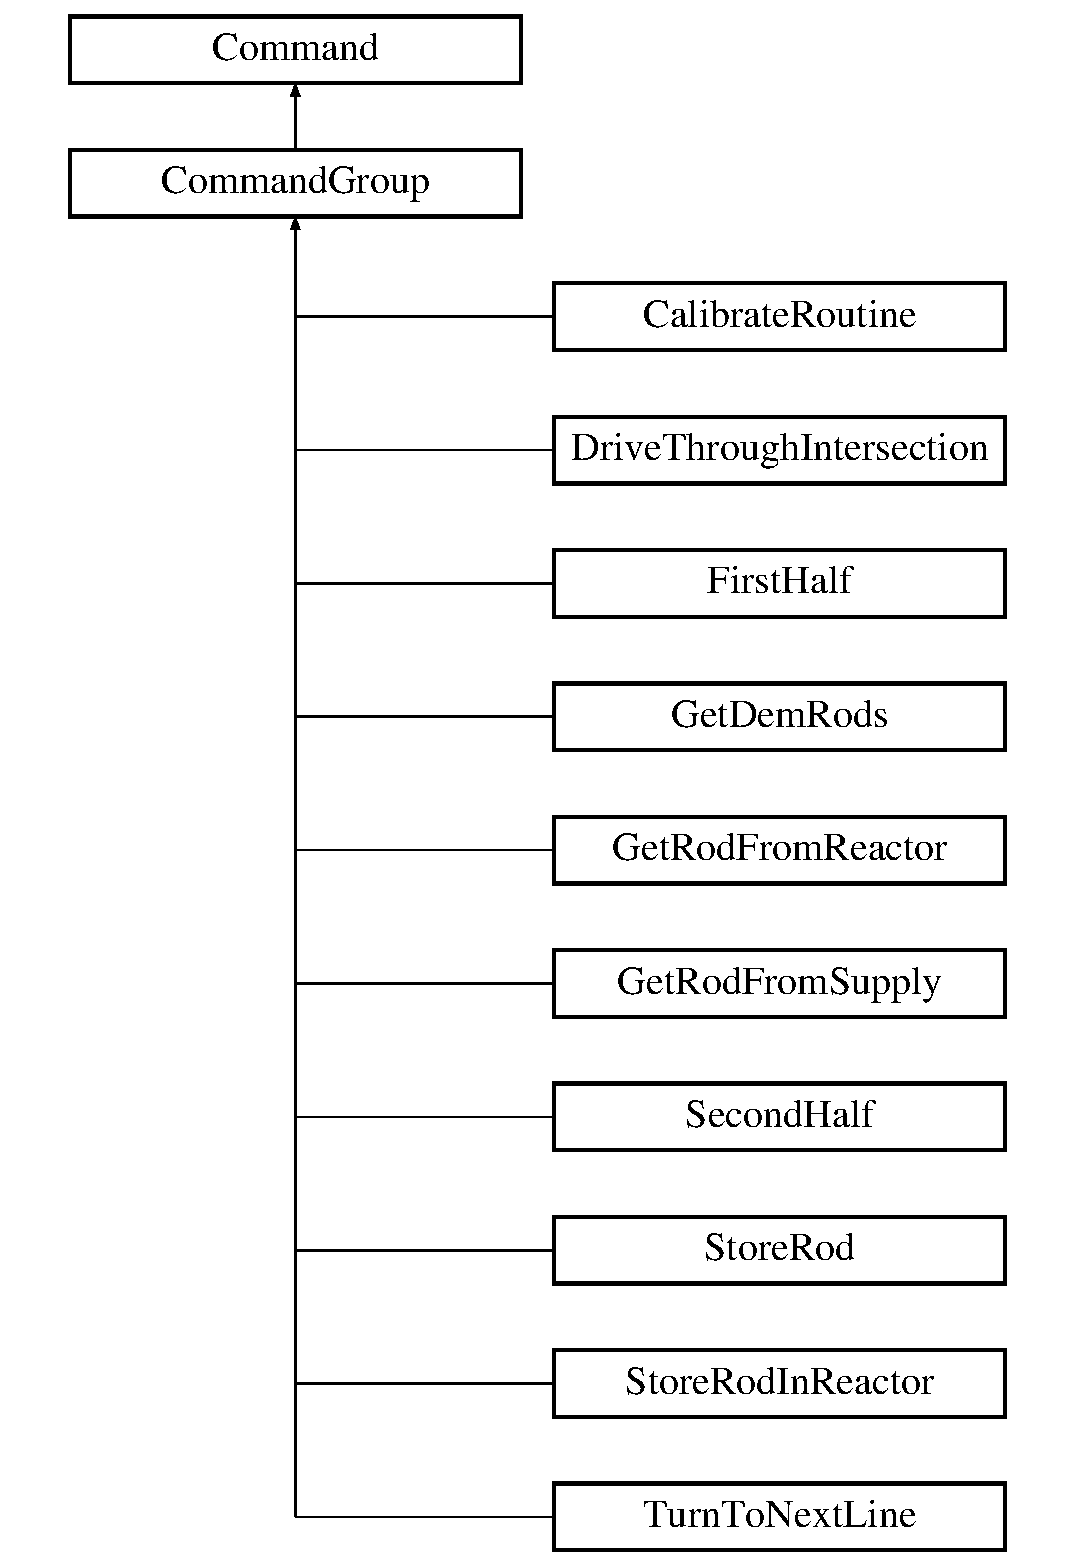
\includegraphics[height=11.000000cm]{classCommandGroup}
\end{center}
\end{figure}
\subsection*{Public Member Functions}
\begin{DoxyCompactItemize}
\item 
\hyperlink{classCommandGroup_a0167d59d8a96fbc0c1999f19610c7358}{Command\-Group} (const String \hyperlink{classCommand_a19f7ad73ca8599ad47f9b7bcccc52610}{name})
\item 
\hyperlink{classCommandGroup_a7b85f5b297c50c9466276c59804ed196}{Command\-Group} ()=default
\item 
void \hyperlink{classCommandGroup_a6b75192504dc74794651e0d82bb83488}{add\-Sequential} (\hyperlink{classCommand}{Command} $\ast$command)
\item 
void \hyperlink{classCommandGroup_a8709a47f6f44a6993cd9f705b360054b}{add\-Parallel} (\hyperlink{classCommand}{Command} $\ast$command)
\item 
virtual void \hyperlink{classCommandGroup_aad0c9576993f9f8d2431cd44f0bf0072}{\-\_\-initialize} ()
\item 
virtual void \hyperlink{classCommandGroup_a09355b6bb1018bdadaa0f5a1c0dec007}{\-\_\-execute} ()
\item 
virtual void \hyperlink{classCommandGroup_a11f0ae6eb2ba052138d5a8930f23bb4f}{\-\_\-end} ()
\item 
virtual void \hyperlink{classCommandGroup_a99800c5dbd05ab750aa0bb27518d0467}{initialize} ()
\begin{DoxyCompactList}\small\item\em run once in the first iteration of the command's life. this will be overrided by individual commands \end{DoxyCompactList}\item 
virtual void \hyperlink{classCommandGroup_a5e91d370cafde43548d79945ccb4d8fe}{execute} ()
\begin{DoxyCompactList}\small\item\em stuff to do over and over each iteration. this will be overrided by individual commands \end{DoxyCompactList}\item 
virtual void \hyperlink{classCommandGroup_a28ad3a1c2f6b4f9aea10efa1a824895e}{end} ()
\begin{DoxyCompactList}\small\item\em called once at the end, once \hyperlink{classCommandGroup_a96807a2763adf9e21ebf2cb9e3574e3c}{is\-Finished()} returned true. this will be overrided by individual commands. \end{DoxyCompactList}\item 
virtual bool \hyperlink{classCommandGroup_a96807a2763adf9e21ebf2cb9e3574e3c}{is\-Finished} ()
\begin{DoxyCompactList}\small\item\em checked every iteration to see if we're done here. this will be overrided by individual commands \end{DoxyCompactList}\end{DoxyCompactItemize}
\subsection*{Public Attributes}
\begin{DoxyCompactItemize}
\item 
\hyperlink{classLinkedList}{Linked\-List}$<$ \hyperlink{classCommandGroupEntry}{Command\-Group\-Entry} $>$ \hyperlink{classCommandGroup_a5906e7052c71befb25842e1f6c55e0b8}{commands}
\end{DoxyCompactItemize}
\subsection*{Private Attributes}
\begin{DoxyCompactItemize}
\item 
int \hyperlink{classCommandGroup_aeb8729b909aafeb23eafcfd0eec22c71}{current\-Command\-Index}
\end{DoxyCompactItemize}


\subsection{Detailed Description}
grouping commands is a useful abstraction. Commands groups execute commands in parallel or series 

Definition at line 10 of file Command\-Group.\-h.



\subsection{Constructor \& Destructor Documentation}
\hypertarget{classCommandGroup_a0167d59d8a96fbc0c1999f19610c7358}{\index{Command\-Group@{Command\-Group}!Command\-Group@{Command\-Group}}
\index{Command\-Group@{Command\-Group}!CommandGroup@{Command\-Group}}
\subsubsection[{Command\-Group}]{\setlength{\rightskip}{0pt plus 5cm}Command\-Group\-::\-Command\-Group (
\begin{DoxyParamCaption}
\item[{const String}]{name}
\end{DoxyParamCaption}
)}}\label{classCommandGroup_a0167d59d8a96fbc0c1999f19610c7358}


Definition at line 4 of file Command\-Group.\-cpp.

\hypertarget{classCommandGroup_a7b85f5b297c50c9466276c59804ed196}{\index{Command\-Group@{Command\-Group}!Command\-Group@{Command\-Group}}
\index{Command\-Group@{Command\-Group}!CommandGroup@{Command\-Group}}
\subsubsection[{Command\-Group}]{\setlength{\rightskip}{0pt plus 5cm}Command\-Group\-::\-Command\-Group (
\begin{DoxyParamCaption}
{}
\end{DoxyParamCaption}
)\hspace{0.3cm}{\ttfamily [default]}}}\label{classCommandGroup_a7b85f5b297c50c9466276c59804ed196}


\subsection{Member Function Documentation}
\hypertarget{classCommandGroup_a11f0ae6eb2ba052138d5a8930f23bb4f}{\index{Command\-Group@{Command\-Group}!\-\_\-end@{\-\_\-end}}
\index{\-\_\-end@{\-\_\-end}!CommandGroup@{Command\-Group}}
\subsubsection[{\-\_\-end}]{\setlength{\rightskip}{0pt plus 5cm}void Command\-Group\-::\-\_\-end (
\begin{DoxyParamCaption}
{}
\end{DoxyParamCaption}
)\hspace{0.3cm}{\ttfamily [virtual]}}}\label{classCommandGroup_a11f0ae6eb2ba052138d5a8930f23bb4f}


Reimplemented from \hyperlink{classCommand_a9173c74652cb69c8807170bf16151ae2}{Command}.



Definition at line 50 of file Command\-Group.\-cpp.

\hypertarget{classCommandGroup_a09355b6bb1018bdadaa0f5a1c0dec007}{\index{Command\-Group@{Command\-Group}!\-\_\-execute@{\-\_\-execute}}
\index{\-\_\-execute@{\-\_\-execute}!CommandGroup@{Command\-Group}}
\subsubsection[{\-\_\-execute}]{\setlength{\rightskip}{0pt plus 5cm}void Command\-Group\-::\-\_\-execute (
\begin{DoxyParamCaption}
{}
\end{DoxyParamCaption}
)\hspace{0.3cm}{\ttfamily [virtual]}}}\label{classCommandGroup_a09355b6bb1018bdadaa0f5a1c0dec007}


Reimplemented from \hyperlink{classCommand_a49e6861e0c14411d6860f0b3211db9c9}{Command}.



Definition at line 22 of file Command\-Group.\-cpp.

\hypertarget{classCommandGroup_aad0c9576993f9f8d2431cd44f0bf0072}{\index{Command\-Group@{Command\-Group}!\-\_\-initialize@{\-\_\-initialize}}
\index{\-\_\-initialize@{\-\_\-initialize}!CommandGroup@{Command\-Group}}
\subsubsection[{\-\_\-initialize}]{\setlength{\rightskip}{0pt plus 5cm}void Command\-Group\-::\-\_\-initialize (
\begin{DoxyParamCaption}
{}
\end{DoxyParamCaption}
)\hspace{0.3cm}{\ttfamily [virtual]}}}\label{classCommandGroup_aad0c9576993f9f8d2431cd44f0bf0072}


Reimplemented from \hyperlink{classCommand_ae7c58ad4895c51ff18f1d432dbd4f4ec}{Command}.



Definition at line 17 of file Command\-Group.\-cpp.

\hypertarget{classCommandGroup_a8709a47f6f44a6993cd9f705b360054b}{\index{Command\-Group@{Command\-Group}!add\-Parallel@{add\-Parallel}}
\index{add\-Parallel@{add\-Parallel}!CommandGroup@{Command\-Group}}
\subsubsection[{add\-Parallel}]{\setlength{\rightskip}{0pt plus 5cm}void Command\-Group\-::add\-Parallel (
\begin{DoxyParamCaption}
\item[{{\bf Command} $\ast$}]{command}
\end{DoxyParamCaption}
)}}\label{classCommandGroup_a8709a47f6f44a6993cd9f705b360054b}


Definition at line 11 of file Command\-Group.\-cpp.

\hypertarget{classCommandGroup_a6b75192504dc74794651e0d82bb83488}{\index{Command\-Group@{Command\-Group}!add\-Sequential@{add\-Sequential}}
\index{add\-Sequential@{add\-Sequential}!CommandGroup@{Command\-Group}}
\subsubsection[{add\-Sequential}]{\setlength{\rightskip}{0pt plus 5cm}void Command\-Group\-::add\-Sequential (
\begin{DoxyParamCaption}
\item[{{\bf Command} $\ast$}]{command}
\end{DoxyParamCaption}
)}}\label{classCommandGroup_a6b75192504dc74794651e0d82bb83488}


Definition at line 6 of file Command\-Group.\-cpp.

\hypertarget{classCommandGroup_a28ad3a1c2f6b4f9aea10efa1a824895e}{\index{Command\-Group@{Command\-Group}!end@{end}}
\index{end@{end}!CommandGroup@{Command\-Group}}
\subsubsection[{end}]{\setlength{\rightskip}{0pt plus 5cm}void Command\-Group\-::end (
\begin{DoxyParamCaption}
{}
\end{DoxyParamCaption}
)\hspace{0.3cm}{\ttfamily [virtual]}}}\label{classCommandGroup_a28ad3a1c2f6b4f9aea10efa1a824895e}


called once at the end, once \hyperlink{classCommandGroup_a96807a2763adf9e21ebf2cb9e3574e3c}{is\-Finished()} returned true. this will be overrided by individual commands. 



Implements \hyperlink{classCommand_abed8b7871ba1078bc10056cac5b471be}{Command}.



Reimplemented in \hyperlink{classGetRodFromReactor_a8d375cbbf822ea0f22058a264347bd37}{Get\-Rod\-From\-Reactor}, and \hyperlink{classStoreRod_a2fe691b28cb7c6942242caa35e43eecb}{Store\-Rod}.



Definition at line 49 of file Command\-Group.\-cpp.

\hypertarget{classCommandGroup_a5e91d370cafde43548d79945ccb4d8fe}{\index{Command\-Group@{Command\-Group}!execute@{execute}}
\index{execute@{execute}!CommandGroup@{Command\-Group}}
\subsubsection[{execute}]{\setlength{\rightskip}{0pt plus 5cm}void Command\-Group\-::execute (
\begin{DoxyParamCaption}
{}
\end{DoxyParamCaption}
)\hspace{0.3cm}{\ttfamily [virtual]}}}\label{classCommandGroup_a5e91d370cafde43548d79945ccb4d8fe}


stuff to do over and over each iteration. this will be overrided by individual commands 



Implements \hyperlink{classCommand_a6fd7d9bd8df8bfc881e4d6c7cd1878b7}{Command}.



Definition at line 21 of file Command\-Group.\-cpp.

\hypertarget{classCommandGroup_a99800c5dbd05ab750aa0bb27518d0467}{\index{Command\-Group@{Command\-Group}!initialize@{initialize}}
\index{initialize@{initialize}!CommandGroup@{Command\-Group}}
\subsubsection[{initialize}]{\setlength{\rightskip}{0pt plus 5cm}void Command\-Group\-::initialize (
\begin{DoxyParamCaption}
{}
\end{DoxyParamCaption}
)\hspace{0.3cm}{\ttfamily [virtual]}}}\label{classCommandGroup_a99800c5dbd05ab750aa0bb27518d0467}


run once in the first iteration of the command's life. this will be overrided by individual commands 



Implements \hyperlink{classCommand_af186abe582ab15ac64750e4b5d7944de}{Command}.



Definition at line 16 of file Command\-Group.\-cpp.

\hypertarget{classCommandGroup_a96807a2763adf9e21ebf2cb9e3574e3c}{\index{Command\-Group@{Command\-Group}!is\-Finished@{is\-Finished}}
\index{is\-Finished@{is\-Finished}!CommandGroup@{Command\-Group}}
\subsubsection[{is\-Finished}]{\setlength{\rightskip}{0pt plus 5cm}bool Command\-Group\-::is\-Finished (
\begin{DoxyParamCaption}
{}
\end{DoxyParamCaption}
)\hspace{0.3cm}{\ttfamily [virtual]}}}\label{classCommandGroup_a96807a2763adf9e21ebf2cb9e3574e3c}


checked every iteration to see if we're done here. this will be overrided by individual commands 

\begin{DoxyReturn}{Returns}
is the function finished 
\end{DoxyReturn}


Implements \hyperlink{classCommand_a9aa704d5f9d98f510a79e645701dc72a}{Command}.



Definition at line 54 of file Command\-Group.\-cpp.



\subsection{Member Data Documentation}
\hypertarget{classCommandGroup_a5906e7052c71befb25842e1f6c55e0b8}{\index{Command\-Group@{Command\-Group}!commands@{commands}}
\index{commands@{commands}!CommandGroup@{Command\-Group}}
\subsubsection[{commands}]{\setlength{\rightskip}{0pt plus 5cm}{\bf Linked\-List}$<${\bf Command\-Group\-Entry}$>$ Command\-Group\-::commands}}\label{classCommandGroup_a5906e7052c71befb25842e1f6c55e0b8}


Definition at line 26 of file Command\-Group.\-h.

\hypertarget{classCommandGroup_aeb8729b909aafeb23eafcfd0eec22c71}{\index{Command\-Group@{Command\-Group}!current\-Command\-Index@{current\-Command\-Index}}
\index{current\-Command\-Index@{current\-Command\-Index}!CommandGroup@{Command\-Group}}
\subsubsection[{current\-Command\-Index}]{\setlength{\rightskip}{0pt plus 5cm}int Command\-Group\-::current\-Command\-Index\hspace{0.3cm}{\ttfamily [private]}}}\label{classCommandGroup_aeb8729b909aafeb23eafcfd0eec22c71}


Definition at line 30 of file Command\-Group.\-h.



The documentation for this class was generated from the following files\-:\begin{DoxyCompactItemize}
\item 
Final\-\_\-\-Project/\hyperlink{CommandGroup_8h}{Command\-Group.\-h}\item 
Final\-\_\-\-Project/\hyperlink{CommandGroup_8cpp}{Command\-Group.\-cpp}\end{DoxyCompactItemize}

\hypertarget{classCommandGroupEntry}{\section{Command\-Group\-Entry Class Reference}
\label{classCommandGroupEntry}\index{Command\-Group\-Entry@{Command\-Group\-Entry}}
}


{\ttfamily \#include $<$Command\-Group\-Entry.\-h$>$}

\subsection*{Public Types}
\begin{DoxyCompactItemize}
\item 
enum \hyperlink{classCommandGroupEntry_a0c435eb6049bef341e92b3550e8f20b1}{Sequence} \{ \hyperlink{classCommandGroupEntry_a0c435eb6049bef341e92b3550e8f20b1a88aa8647af6ba782f9faf0eb8986a730}{k\-Sequence\-\_\-\-In\-Sequence}, 
\hyperlink{classCommandGroupEntry_a0c435eb6049bef341e92b3550e8f20b1a1576e3e1f5d8e12f32ebacb248fee63e}{k\-Sequence\-\_\-\-In\-Parallel}
 \}
\end{DoxyCompactItemize}
\subsection*{Public Member Functions}
\begin{DoxyCompactItemize}
\item 
\hyperlink{classCommandGroupEntry_a64e939b3d002d394ed63079f74fbf144}{Command\-Group\-Entry} ()=default
\item 
\hyperlink{classCommandGroupEntry_a638a9b82f73e4aa5b268eaad4a1c95de}{Command\-Group\-Entry} (\hyperlink{classCommand}{Command} $\ast$command, \hyperlink{classCommandGroupEntry_a0c435eb6049bef341e92b3550e8f20b1}{Sequence} state)
\item 
bool \hyperlink{classCommandGroupEntry_ad12a901f2d52aa1da54020c118f222a5}{operator!=} (const \hyperlink{classCommandGroupEntry}{Command\-Group\-Entry} \&other)
\end{DoxyCompactItemize}
\subsection*{Public Attributes}
\begin{DoxyCompactItemize}
\item 
\hyperlink{classCommand}{Command} $\ast$ \hyperlink{classCommandGroupEntry_a466202de6dd9aed12db553da04c726b2}{\-\_\-command} = N\-U\-L\-L
\item 
\hyperlink{classCommandGroupEntry_a0c435eb6049bef341e92b3550e8f20b1}{Sequence} \hyperlink{classCommandGroupEntry_a3a011ee2d2c871fce8a37dd3cb3d1ddf}{\-\_\-state} = \hyperlink{classCommandGroupEntry_a0c435eb6049bef341e92b3550e8f20b1a88aa8647af6ba782f9faf0eb8986a730}{k\-Sequence\-\_\-\-In\-Sequence}
\end{DoxyCompactItemize}


\subsection{Detailed Description}


Definition at line 7 of file Command\-Group\-Entry.\-h.



\subsection{Member Enumeration Documentation}
\hypertarget{classCommandGroupEntry_a0c435eb6049bef341e92b3550e8f20b1}{\index{Command\-Group\-Entry@{Command\-Group\-Entry}!Sequence@{Sequence}}
\index{Sequence@{Sequence}!CommandGroupEntry@{Command\-Group\-Entry}}
\subsubsection[{Sequence}]{\setlength{\rightskip}{0pt plus 5cm}enum {\bf Command\-Group\-Entry\-::\-Sequence}}}\label{classCommandGroupEntry_a0c435eb6049bef341e92b3550e8f20b1}
\begin{Desc}
\item[Enumerator]\par
\begin{description}
\index{k\-Sequence\-\_\-\-In\-Sequence@{k\-Sequence\-\_\-\-In\-Sequence}!Command\-Group\-Entry@{Command\-Group\-Entry}}\index{Command\-Group\-Entry@{Command\-Group\-Entry}!k\-Sequence\-\_\-\-In\-Sequence@{k\-Sequence\-\_\-\-In\-Sequence}}\item[{\em 
\hypertarget{classCommandGroupEntry_a0c435eb6049bef341e92b3550e8f20b1a88aa8647af6ba782f9faf0eb8986a730}{k\-Sequence\-\_\-\-In\-Sequence}\label{classCommandGroupEntry_a0c435eb6049bef341e92b3550e8f20b1a88aa8647af6ba782f9faf0eb8986a730}
}]\index{k\-Sequence\-\_\-\-In\-Parallel@{k\-Sequence\-\_\-\-In\-Parallel}!Command\-Group\-Entry@{Command\-Group\-Entry}}\index{Command\-Group\-Entry@{Command\-Group\-Entry}!k\-Sequence\-\_\-\-In\-Parallel@{k\-Sequence\-\_\-\-In\-Parallel}}\item[{\em 
\hypertarget{classCommandGroupEntry_a0c435eb6049bef341e92b3550e8f20b1a1576e3e1f5d8e12f32ebacb248fee63e}{k\-Sequence\-\_\-\-In\-Parallel}\label{classCommandGroupEntry_a0c435eb6049bef341e92b3550e8f20b1a1576e3e1f5d8e12f32ebacb248fee63e}
}]\end{description}
\end{Desc}


Definition at line 9 of file Command\-Group\-Entry.\-h.



\subsection{Constructor \& Destructor Documentation}
\hypertarget{classCommandGroupEntry_a64e939b3d002d394ed63079f74fbf144}{\index{Command\-Group\-Entry@{Command\-Group\-Entry}!Command\-Group\-Entry@{Command\-Group\-Entry}}
\index{Command\-Group\-Entry@{Command\-Group\-Entry}!CommandGroupEntry@{Command\-Group\-Entry}}
\subsubsection[{Command\-Group\-Entry}]{\setlength{\rightskip}{0pt plus 5cm}Command\-Group\-Entry\-::\-Command\-Group\-Entry (
\begin{DoxyParamCaption}
{}
\end{DoxyParamCaption}
)\hspace{0.3cm}{\ttfamily [default]}}}\label{classCommandGroupEntry_a64e939b3d002d394ed63079f74fbf144}
\hypertarget{classCommandGroupEntry_a638a9b82f73e4aa5b268eaad4a1c95de}{\index{Command\-Group\-Entry@{Command\-Group\-Entry}!Command\-Group\-Entry@{Command\-Group\-Entry}}
\index{Command\-Group\-Entry@{Command\-Group\-Entry}!CommandGroupEntry@{Command\-Group\-Entry}}
\subsubsection[{Command\-Group\-Entry}]{\setlength{\rightskip}{0pt plus 5cm}Command\-Group\-Entry\-::\-Command\-Group\-Entry (
\begin{DoxyParamCaption}
\item[{{\bf Command} $\ast$}]{command, }
\item[{{\bf Command\-Group\-Entry\-::\-Sequence}}]{state}
\end{DoxyParamCaption}
)}}\label{classCommandGroupEntry_a638a9b82f73e4aa5b268eaad4a1c95de}


Definition at line 4 of file Command\-Group\-Entry.\-cpp.



\subsection{Member Function Documentation}
\hypertarget{classCommandGroupEntry_ad12a901f2d52aa1da54020c118f222a5}{\index{Command\-Group\-Entry@{Command\-Group\-Entry}!operator!=@{operator!=}}
\index{operator!=@{operator!=}!CommandGroupEntry@{Command\-Group\-Entry}}
\subsubsection[{operator!=}]{\setlength{\rightskip}{0pt plus 5cm}bool Command\-Group\-Entry\-::operator!= (
\begin{DoxyParamCaption}
\item[{const {\bf Command\-Group\-Entry} \&}]{other}
\end{DoxyParamCaption}
)}}\label{classCommandGroupEntry_ad12a901f2d52aa1da54020c118f222a5}


Definition at line 9 of file Command\-Group\-Entry.\-cpp.



\subsection{Member Data Documentation}
\hypertarget{classCommandGroupEntry_a466202de6dd9aed12db553da04c726b2}{\index{Command\-Group\-Entry@{Command\-Group\-Entry}!\-\_\-command@{\-\_\-command}}
\index{\-\_\-command@{\-\_\-command}!CommandGroupEntry@{Command\-Group\-Entry}}
\subsubsection[{\-\_\-command}]{\setlength{\rightskip}{0pt plus 5cm}{\bf Command}$\ast$ Command\-Group\-Entry\-::\-\_\-command = N\-U\-L\-L}}\label{classCommandGroupEntry_a466202de6dd9aed12db553da04c726b2}


Definition at line 19 of file Command\-Group\-Entry.\-h.

\hypertarget{classCommandGroupEntry_a3a011ee2d2c871fce8a37dd3cb3d1ddf}{\index{Command\-Group\-Entry@{Command\-Group\-Entry}!\-\_\-state@{\-\_\-state}}
\index{\-\_\-state@{\-\_\-state}!CommandGroupEntry@{Command\-Group\-Entry}}
\subsubsection[{\-\_\-state}]{\setlength{\rightskip}{0pt plus 5cm}{\bf Sequence} Command\-Group\-Entry\-::\-\_\-state = {\bf k\-Sequence\-\_\-\-In\-Sequence}}}\label{classCommandGroupEntry_a3a011ee2d2c871fce8a37dd3cb3d1ddf}


Definition at line 20 of file Command\-Group\-Entry.\-h.



The documentation for this class was generated from the following files\-:\begin{DoxyCompactItemize}
\item 
Final\-\_\-\-Project/\hyperlink{CommandGroupEntry_8h}{Command\-Group\-Entry.\-h}\item 
Final\-\_\-\-Project/\hyperlink{CommandGroupEntry_8cpp}{Command\-Group\-Entry.\-cpp}\end{DoxyCompactItemize}

\hypertarget{classDriveUntilIntersection}{\section{Drive\-Until\-Intersection Class Reference}
\label{classDriveUntilIntersection}\index{Drive\-Until\-Intersection@{Drive\-Until\-Intersection}}
}
Inheritance diagram for Drive\-Until\-Intersection\-:\begin{figure}[H]
\begin{center}
\leavevmode
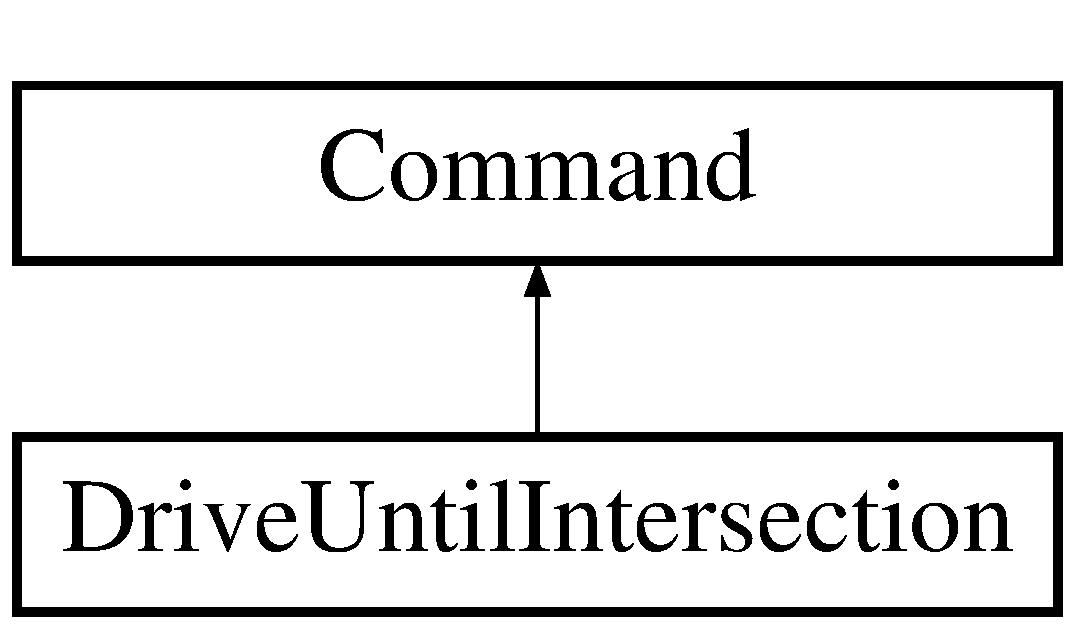
\includegraphics[height=2.000000cm]{classDriveUntilIntersection}
\end{center}
\end{figure}
\subsection*{Public Member Functions}
\begin{DoxyCompactItemize}
\item 
\hypertarget{classDriveUntilIntersection_a7f42c796bcea682dea57f1439cc59f7b}{void \hyperlink{classDriveUntilIntersection_a7f42c796bcea682dea57f1439cc59f7b}{initialize} ()}\label{classDriveUntilIntersection_a7f42c796bcea682dea57f1439cc59f7b}

\begin{DoxyCompactList}\small\item\em run once in the first iteration of the command's life. this will be overrided by individual commands \end{DoxyCompactList}\item 
\hypertarget{classDriveUntilIntersection_ae670d4da34843889558d42c94fc1e292}{void \hyperlink{classDriveUntilIntersection_ae670d4da34843889558d42c94fc1e292}{execute} ()}\label{classDriveUntilIntersection_ae670d4da34843889558d42c94fc1e292}

\begin{DoxyCompactList}\small\item\em stuff to do over and over each iteration. this will be overrided by individual commands \end{DoxyCompactList}\item 
bool \hyperlink{classDriveUntilIntersection_a345809c722142166801f6ecbca117758}{is\-Finished} ()
\begin{DoxyCompactList}\small\item\em checked every iteration to see if we're done here. this will be overrided by individual commands \end{DoxyCompactList}\item 
\hypertarget{classDriveUntilIntersection_a309d1f37d92844707c2f3dcb2f5d5638}{void \hyperlink{classDriveUntilIntersection_a309d1f37d92844707c2f3dcb2f5d5638}{end} ()}\label{classDriveUntilIntersection_a309d1f37d92844707c2f3dcb2f5d5638}

\begin{DoxyCompactList}\small\item\em called once at the end, once \hyperlink{classDriveUntilIntersection_a345809c722142166801f6ecbca117758}{is\-Finished()} returned true. this will be overrided by individual commands. \end{DoxyCompactList}\end{DoxyCompactItemize}
\subsection*{Additional Inherited Members}


\subsection{Member Function Documentation}
\hypertarget{classDriveUntilIntersection_a345809c722142166801f6ecbca117758}{\index{Drive\-Until\-Intersection@{Drive\-Until\-Intersection}!is\-Finished@{is\-Finished}}
\index{is\-Finished@{is\-Finished}!DriveUntilIntersection@{Drive\-Until\-Intersection}}
\subsubsection[{is\-Finished}]{\setlength{\rightskip}{0pt plus 5cm}bool Drive\-Until\-Intersection\-::is\-Finished (
\begin{DoxyParamCaption}
{}
\end{DoxyParamCaption}
)\hspace{0.3cm}{\ttfamily [virtual]}}}\label{classDriveUntilIntersection_a345809c722142166801f6ecbca117758}


checked every iteration to see if we're done here. this will be overrided by individual commands 

\begin{DoxyReturn}{Returns}
is the function finished 
\end{DoxyReturn}


Implements \hyperlink{classCommand_a9aa704d5f9d98f510a79e645701dc72a}{Command}.



The documentation for this class was generated from the following files\-:\begin{DoxyCompactItemize}
\item 
Final\-\_\-\-Project/Drive\-Until\-Intersection.\-h\item 
Final\-\_\-\-Project/Drive\-Until\-Intersection.\-cpp\end{DoxyCompactItemize}

\hypertarget{classGetDemRods}{\section{Get\-Dem\-Rods Class Reference}
\label{classGetDemRods}\index{Get\-Dem\-Rods@{Get\-Dem\-Rods}}
}
Inheritance diagram for Get\-Dem\-Rods\-:\begin{figure}[H]
\begin{center}
\leavevmode
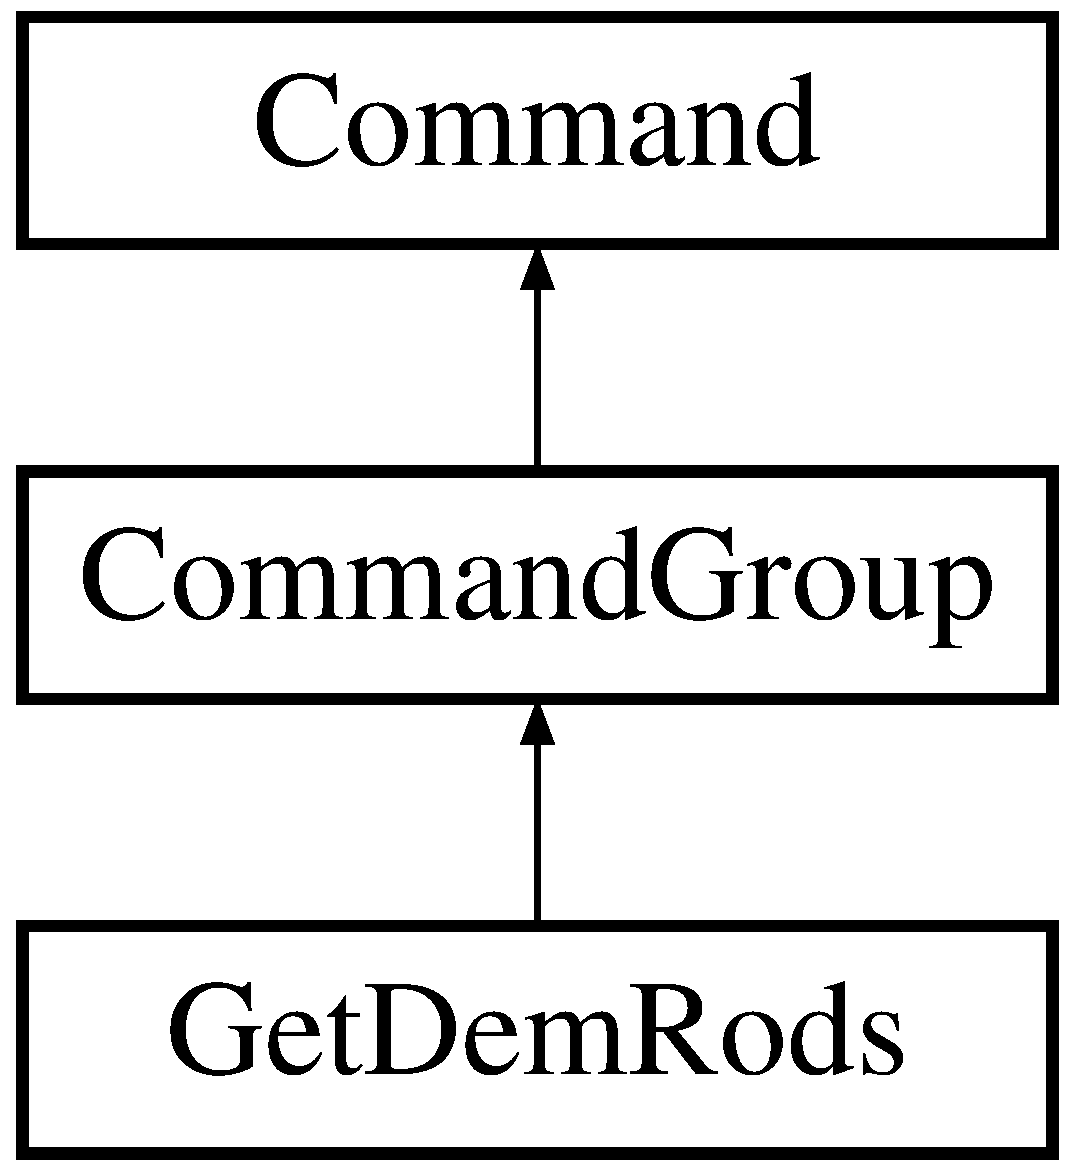
\includegraphics[height=3.000000cm]{classGetDemRods}
\end{center}
\end{figure}
\subsection*{Additional Inherited Members}


The documentation for this class was generated from the following files\-:\begin{DoxyCompactItemize}
\item 
Final\-\_\-\-Project/Get\-Dem\-Rods.\-h\item 
Final\-\_\-\-Project/Get\-Dem\-Rods.\-cpp\end{DoxyCompactItemize}

\hypertarget{classGetRodFromReactor}{\section{Get\-Rod\-From\-Reactor Class Reference}
\label{classGetRodFromReactor}\index{Get\-Rod\-From\-Reactor@{Get\-Rod\-From\-Reactor}}
}
Inheritance diagram for Get\-Rod\-From\-Reactor\-:\begin{figure}[H]
\begin{center}
\leavevmode
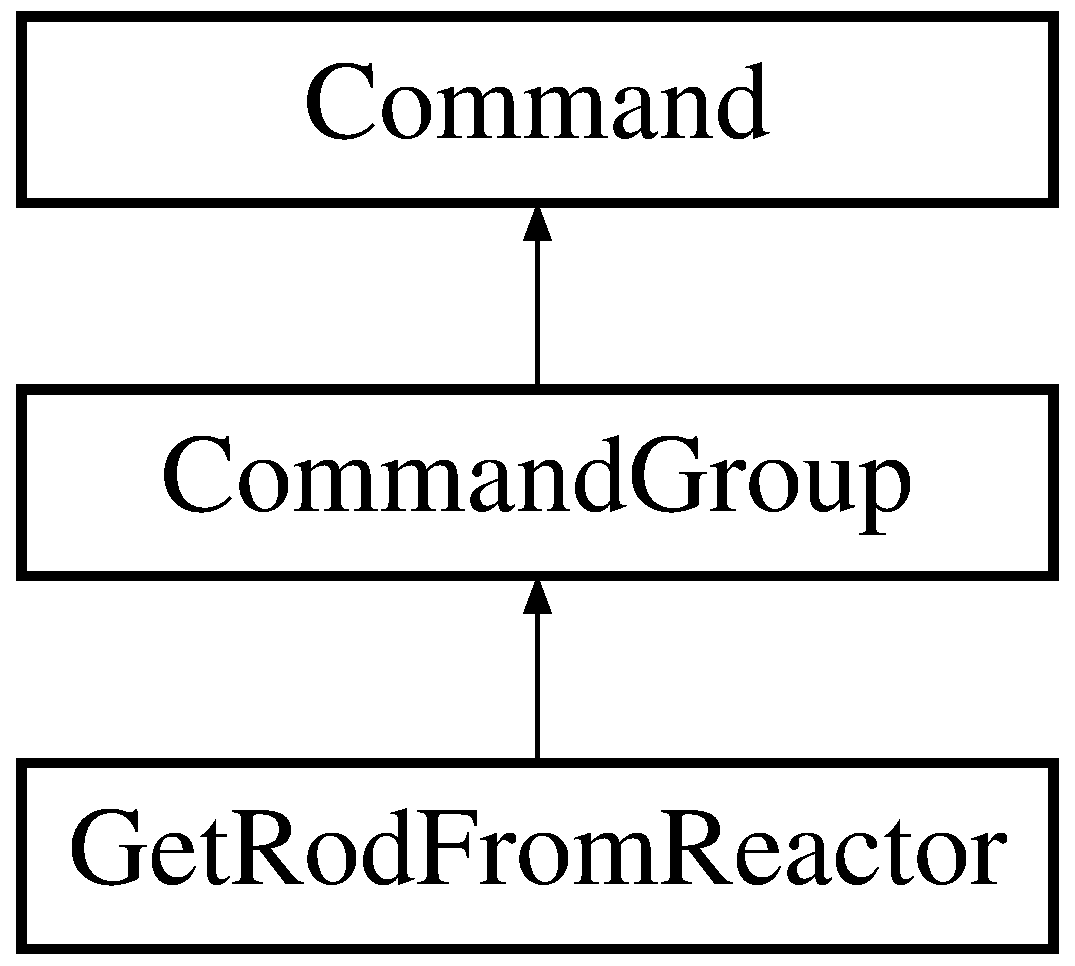
\includegraphics[height=3.000000cm]{classGetRodFromReactor}
\end{center}
\end{figure}
\subsection*{Public Member Functions}
\begin{DoxyCompactItemize}
\item 
\hypertarget{classGetRodFromReactor_ae6432d3e1fd6ca0e882d9cbff1b14737}{{\bfseries Get\-Rod\-From\-Reactor} (const int reactor\-Number)}\label{classGetRodFromReactor_ae6432d3e1fd6ca0e882d9cbff1b14737}

\item 
\hypertarget{classGetRodFromReactor_a8d375cbbf822ea0f22058a264347bd37}{void \hyperlink{classGetRodFromReactor_a8d375cbbf822ea0f22058a264347bd37}{end} ()}\label{classGetRodFromReactor_a8d375cbbf822ea0f22058a264347bd37}

\begin{DoxyCompactList}\small\item\em called once at the end, once \hyperlink{classCommandGroup_a96807a2763adf9e21ebf2cb9e3574e3c}{is\-Finished()} returned true. this will be overrided by individual commands. \end{DoxyCompactList}\end{DoxyCompactItemize}
\subsection*{Additional Inherited Members}


The documentation for this class was generated from the following files\-:\begin{DoxyCompactItemize}
\item 
Final\-\_\-\-Project/Get\-Rod\-From\-Reactor.\-h\item 
Final\-\_\-\-Project/Get\-Rod\-From\-Reactor.\-cpp\end{DoxyCompactItemize}

\hypertarget{classGetRodFromSupply}{\section{Get\-Rod\-From\-Supply Class Reference}
\label{classGetRodFromSupply}\index{Get\-Rod\-From\-Supply@{Get\-Rod\-From\-Supply}}
}


{\ttfamily \#include $<$Get\-Rod\-From\-Supply.\-h$>$}

Inheritance diagram for Get\-Rod\-From\-Supply\-:\begin{figure}[H]
\begin{center}
\leavevmode
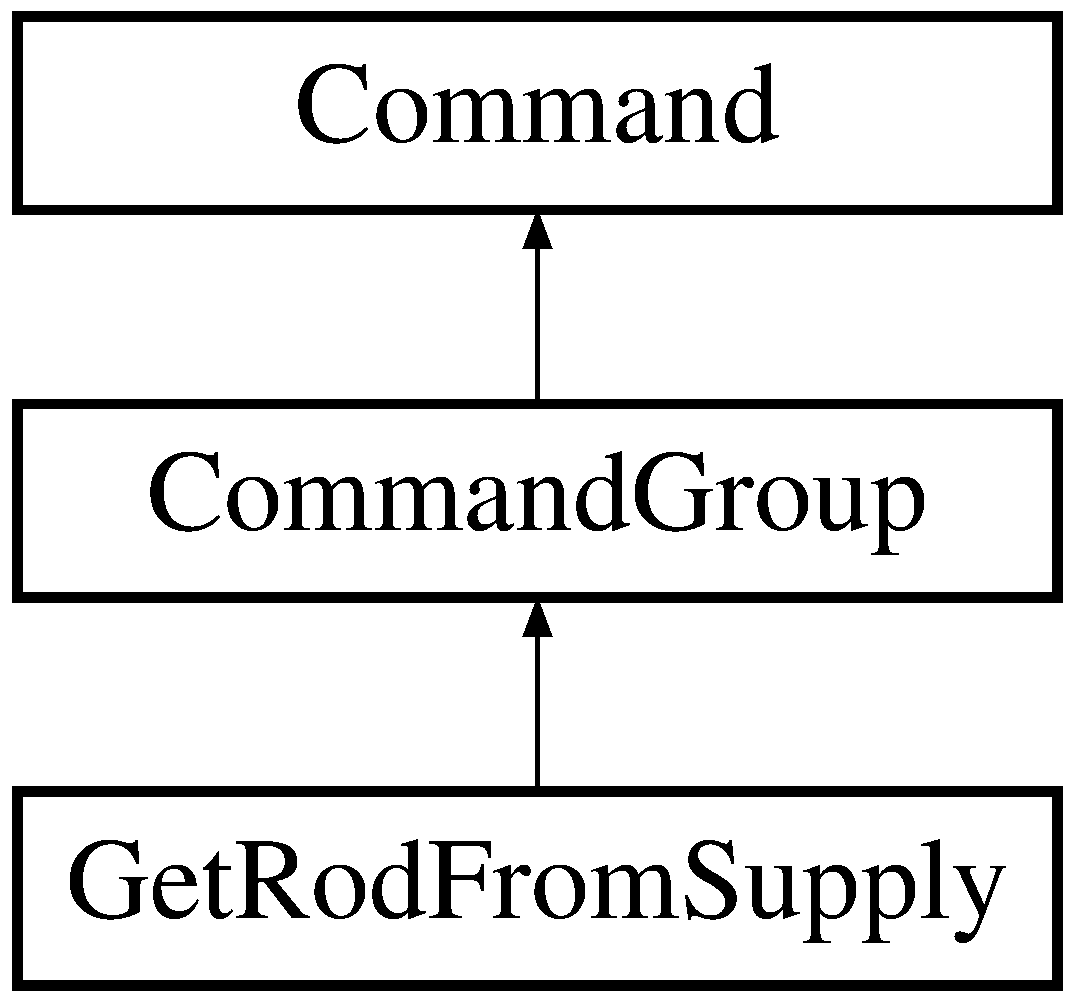
\includegraphics[height=3.000000cm]{classGetRodFromSupply}
\end{center}
\end{figure}
\subsection*{Public Member Functions}
\begin{DoxyCompactItemize}
\item 
\hyperlink{classGetRodFromSupply_a8c06b54ce60f0547d4cb68465081c042}{Get\-Rod\-From\-Supply} ()
\end{DoxyCompactItemize}
\subsection*{Additional Inherited Members}


\subsection{Detailed Description}


Definition at line 6 of file Get\-Rod\-From\-Supply.\-h.



\subsection{Constructor \& Destructor Documentation}
\hypertarget{classGetRodFromSupply_a8c06b54ce60f0547d4cb68465081c042}{\index{Get\-Rod\-From\-Supply@{Get\-Rod\-From\-Supply}!Get\-Rod\-From\-Supply@{Get\-Rod\-From\-Supply}}
\index{Get\-Rod\-From\-Supply@{Get\-Rod\-From\-Supply}!GetRodFromSupply@{Get\-Rod\-From\-Supply}}
\subsubsection[{Get\-Rod\-From\-Supply}]{\setlength{\rightskip}{0pt plus 5cm}Get\-Rod\-From\-Supply\-::\-Get\-Rod\-From\-Supply (
\begin{DoxyParamCaption}
{}
\end{DoxyParamCaption}
)}}\label{classGetRodFromSupply_a8c06b54ce60f0547d4cb68465081c042}


Definition at line 9 of file Get\-Rod\-From\-Supply.\-cpp.



The documentation for this class was generated from the following files\-:\begin{DoxyCompactItemize}
\item 
Final\-\_\-\-Project/\hyperlink{GetRodFromSupply_8h}{Get\-Rod\-From\-Supply.\-h}\item 
Final\-\_\-\-Project/\hyperlink{GetRodFromSupply_8cpp}{Get\-Rod\-From\-Supply.\-cpp}\end{DoxyCompactItemize}

\hypertarget{classGripper}{\section{Gripper Class Reference}
\label{classGripper}\index{Gripper@{Gripper}}
}


{\ttfamily \#include $<$Gripper.\-h$>$}

\subsection*{Public Member Functions}
\begin{DoxyCompactItemize}
\item 
void \hyperlink{classGripper_a7eff7781d1109b4e988fa66c8141a6d7}{setup} ()
\item 
void \hyperlink{classGripper_ada511826dbf5abcdd12532ae725efeaf}{cls} ()
\begin{DoxyCompactList}\small\item\em close the gripper \end{DoxyCompactList}\item 
void \hyperlink{classGripper_ab4fa689ad3f08e97c7fcd10247965ff5}{opn} ()
\begin{DoxyCompactList}\small\item\em open the gripper \end{DoxyCompactList}\end{DoxyCompactItemize}
\subsection*{Public Attributes}
\begin{DoxyCompactItemize}
\item 
Servo \hyperlink{classGripper_ad72d0ae4ccd2be00ec3f303e7a0c1cc9}{motor}
\end{DoxyCompactItemize}
\subsection*{Static Public Attributes}
\begin{DoxyCompactItemize}
\item 
static const int \hyperlink{classGripper_ae12467d04d155401f1c6ba694b295f40}{motor\-Pin} = 6
\end{DoxyCompactItemize}


\subsection{Detailed Description}


Definition at line 7 of file Gripper.\-h.



\subsection{Member Function Documentation}
\hypertarget{classGripper_ada511826dbf5abcdd12532ae725efeaf}{\index{Gripper@{Gripper}!cls@{cls}}
\index{cls@{cls}!Gripper@{Gripper}}
\subsubsection[{cls}]{\setlength{\rightskip}{0pt plus 5cm}void Gripper\-::cls (
\begin{DoxyParamCaption}
{}
\end{DoxyParamCaption}
)}}\label{classGripper_ada511826dbf5abcdd12532ae725efeaf}


close the gripper 



Definition at line 10 of file Gripper.\-cpp.

\hypertarget{classGripper_ab4fa689ad3f08e97c7fcd10247965ff5}{\index{Gripper@{Gripper}!opn@{opn}}
\index{opn@{opn}!Gripper@{Gripper}}
\subsubsection[{opn}]{\setlength{\rightskip}{0pt plus 5cm}void Gripper\-::opn (
\begin{DoxyParamCaption}
{}
\end{DoxyParamCaption}
)}}\label{classGripper_ab4fa689ad3f08e97c7fcd10247965ff5}


open the gripper 



Definition at line 15 of file Gripper.\-cpp.

\hypertarget{classGripper_a7eff7781d1109b4e988fa66c8141a6d7}{\index{Gripper@{Gripper}!setup@{setup}}
\index{setup@{setup}!Gripper@{Gripper}}
\subsubsection[{setup}]{\setlength{\rightskip}{0pt plus 5cm}void Gripper\-::setup (
\begin{DoxyParamCaption}
{}
\end{DoxyParamCaption}
)}}\label{classGripper_a7eff7781d1109b4e988fa66c8141a6d7}


Definition at line 6 of file Gripper.\-cpp.



\subsection{Member Data Documentation}
\hypertarget{classGripper_ad72d0ae4ccd2be00ec3f303e7a0c1cc9}{\index{Gripper@{Gripper}!motor@{motor}}
\index{motor@{motor}!Gripper@{Gripper}}
\subsubsection[{motor}]{\setlength{\rightskip}{0pt plus 5cm}Servo Gripper\-::motor}}\label{classGripper_ad72d0ae4ccd2be00ec3f303e7a0c1cc9}


Definition at line 18 of file Gripper.\-h.

\hypertarget{classGripper_ae12467d04d155401f1c6ba694b295f40}{\index{Gripper@{Gripper}!motor\-Pin@{motor\-Pin}}
\index{motor\-Pin@{motor\-Pin}!Gripper@{Gripper}}
\subsubsection[{motor\-Pin}]{\setlength{\rightskip}{0pt plus 5cm}const int Gripper\-::motor\-Pin = 6\hspace{0.3cm}{\ttfamily [static]}}}\label{classGripper_ae12467d04d155401f1c6ba694b295f40}


Definition at line 19 of file Gripper.\-h.



The documentation for this class was generated from the following files\-:\begin{DoxyCompactItemize}
\item 
Final\-\_\-\-Project/\hyperlink{Gripper_8h}{Gripper.\-h}\item 
Final\-\_\-\-Project/\hyperlink{Gripper_8cpp}{Gripper.\-cpp}\end{DoxyCompactItemize}

\hypertarget{classLineSensor}{\section{Line\-Sensor Class Reference}
\label{classLineSensor}\index{Line\-Sensor@{Line\-Sensor}}
}


functions for reading the position with respect to the line  




{\ttfamily \#include $<$Line\-Sensor.\-h$>$}

\subsection*{Public Member Functions}
\begin{DoxyCompactItemize}
\item 
void \hyperlink{classLineSensor_a555f6f7222ea1e76ed810edbde44c39c}{setup} ()
\begin{DoxyCompactList}\small\item\em setup servos and stuff. called by main setup \end{DoxyCompactList}\item 
bool \hyperlink{classLineSensor_a6769cf781edb7ac4a43086cd62be01e2}{at\-Intersection} ()
\begin{DoxyCompactList}\small\item\em returns true if both sensors are on the line \end{DoxyCompactList}\item 
bool \hyperlink{classLineSensor_ad9d3c5a694f1ff946d1137df1694b026}{on\-Line} ()
\begin{DoxyCompactList}\small\item\em returns if line sensor is on the line \end{DoxyCompactList}\item 
bool \hyperlink{classLineSensor_a0dea8f6d7e7e27d050feecb3e549a149}{off\-Line} ()
\begin{DoxyCompactList}\small\item\em returns if line sensor is off the line \end{DoxyCompactList}\item 
void \hyperlink{classLineSensor_afc809d2aa49426d949f76f68b0154050}{cache} ()
\begin{DoxyCompactList}\small\item\em does raw read and storage of line sensor. This must be caled every loop \end{DoxyCompactList}\item 
int \hyperlink{classLineSensor_a74c3c2d7a454aeacae90501670d01bdc}{adjustment\-Power} ()
\begin{DoxyCompactList}\small\item\em get how much motor power you should adjust by. from -\/100 to 100 \end{DoxyCompactList}\end{DoxyCompactItemize}
\subsection*{Private Attributes}
\begin{DoxyCompactItemize}
\item 
float \hyperlink{classLineSensor_ac21af83a73e9e55500324d9d34ed2498}{line\-Position}
\begin{DoxyCompactList}\small\item\em holds the line position as calculated by cache. On scale of tens \end{DoxyCompactList}\item 
float \hyperlink{classLineSensor_a347e843234a242ded12e83badf4718ed}{last\-Line\-Position}
\item 
const float \hyperlink{classLineSensor_af246497cb5a3386afcc4ce864949c57f}{k\-P} = 8.\-0
\item 
const float \hyperlink{classLineSensor_a62c587ff3d58f72a74ae39429b7d0837}{k\-D} = 1.\-5
\item 
int \hyperlink{classLineSensor_aa5bd7119b2332eab8b6c850f8fa3d558}{derivative}
\item 
int \hyperlink{classLineSensor_af574319adc88f5949f03239b2bcbc222}{sum}
\begin{DoxyCompactList}\small\item\em sum of raw line sensor values. used to detect intersections \end{DoxyCompactList}\end{DoxyCompactItemize}
\subsection*{Static Private Attributes}
\begin{DoxyCompactItemize}
\item 
static const int \hyperlink{classLineSensor_a873c5b45cdfa14ff468db018e1e0055a}{P\-I\-N\-\_\-0} = 0
\begin{DoxyCompactList}\small\item\em this assumes line sensor pins are in order. This is the first (leftmost pin) \end{DoxyCompactList}\item 
static const int \hyperlink{classLineSensor_a09da44442cb9e026af2053b5d0b4f2ce}{L\-E\-D\-P\-I\-N} = 29
\begin{DoxyCompactList}\small\item\em the board contains I\-R L\-E\-Ds, this pin controls those L\-E\-Ds \end{DoxyCompactList}\item 
static const float \hyperlink{classLineSensor_a8db50f7d2c026003180d0c5c7e184d9f}{O\-F\-F\-\_\-\-P\-O\-S\-\_\-\-T\-H\-R\-E\-S\-H\-O\-L\-D} = 1.\-3
\begin{DoxyCompactList}\small\item\em determines what constitutes a black line (from -\/100 to 100) these numbers may be the same, but don't have to be \end{DoxyCompactList}\item 
static const float \hyperlink{classLineSensor_a3e3c5f134159562e56fcd06e55cc7024}{O\-N\-\_\-\-P\-O\-S\-\_\-\-T\-H\-R\-E\-S\-H\-O\-L\-D} = 0.\-6
\item 
static const float \hyperlink{classLineSensor_affb177c49a3381f380b6ff7dd298297f}{C\-O\-M\-P\-E\-N\-S\-A\-T\-I\-O\-N} = 1
\begin{DoxyCompactList}\small\item\em account for broken line sensors \end{DoxyCompactList}\item 
static const int \hyperlink{classLineSensor_a55b9f63bd4c01990f6f2d7baa830d2ec}{I\-N\-T\-E\-R\-S\-E\-C\-T\-I\-O\-N\-\_\-\-T\-H\-R\-E\-S\-H\-O\-L\-D} = 2800
\begin{DoxyCompactList}\small\item\em test if we're at a line \end{DoxyCompactList}\item 
static const int \hyperlink{classLineSensor_a929091ad1746a0a337c2259ba79c959a}{L\-O\-W\-\_\-\-S\-U\-M\-\_\-\-T\-H\-R\-E\-S\-H\-O\-L\-D} = 1000
\item 
static const int \hyperlink{classLineSensor_a3e7f65abc054f54cb74f8aa3eb552e89}{H\-I\-G\-H\-\_\-\-S\-U\-M\-\_\-\-T\-H\-R\-E\-S\-H\-O\-L\-D} = 1600
\end{DoxyCompactItemize}


\subsection{Detailed Description}
functions for reading the position with respect to the line 

Definition at line 6 of file Line\-Sensor.\-h.



\subsection{Member Function Documentation}
\hypertarget{classLineSensor_a74c3c2d7a454aeacae90501670d01bdc}{\index{Line\-Sensor@{Line\-Sensor}!adjustment\-Power@{adjustment\-Power}}
\index{adjustment\-Power@{adjustment\-Power}!LineSensor@{Line\-Sensor}}
\subsubsection[{adjustment\-Power}]{\setlength{\rightskip}{0pt plus 5cm}int Line\-Sensor\-::adjustment\-Power (
\begin{DoxyParamCaption}
{}
\end{DoxyParamCaption}
)}}\label{classLineSensor_a74c3c2d7a454aeacae90501670d01bdc}


get how much motor power you should adjust by. from -\/100 to 100 



Definition at line 25 of file Line\-Sensor.\-cpp.

\hypertarget{classLineSensor_a6769cf781edb7ac4a43086cd62be01e2}{\index{Line\-Sensor@{Line\-Sensor}!at\-Intersection@{at\-Intersection}}
\index{at\-Intersection@{at\-Intersection}!LineSensor@{Line\-Sensor}}
\subsubsection[{at\-Intersection}]{\setlength{\rightskip}{0pt plus 5cm}bool Line\-Sensor\-::at\-Intersection (
\begin{DoxyParamCaption}
{}
\end{DoxyParamCaption}
)}}\label{classLineSensor_a6769cf781edb7ac4a43086cd62be01e2}


returns true if both sensors are on the line 



Definition at line 21 of file Line\-Sensor.\-cpp.

\hypertarget{classLineSensor_afc809d2aa49426d949f76f68b0154050}{\index{Line\-Sensor@{Line\-Sensor}!cache@{cache}}
\index{cache@{cache}!LineSensor@{Line\-Sensor}}
\subsubsection[{cache}]{\setlength{\rightskip}{0pt plus 5cm}void Line\-Sensor\-::cache (
\begin{DoxyParamCaption}
{}
\end{DoxyParamCaption}
)}}\label{classLineSensor_afc809d2aa49426d949f76f68b0154050}


does raw read and storage of line sensor. This must be caled every loop 



Definition at line 8 of file Line\-Sensor.\-cpp.

\hypertarget{classLineSensor_a0dea8f6d7e7e27d050feecb3e549a149}{\index{Line\-Sensor@{Line\-Sensor}!off\-Line@{off\-Line}}
\index{off\-Line@{off\-Line}!LineSensor@{Line\-Sensor}}
\subsubsection[{off\-Line}]{\setlength{\rightskip}{0pt plus 5cm}bool Line\-Sensor\-::off\-Line (
\begin{DoxyParamCaption}
{}
\end{DoxyParamCaption}
)}}\label{classLineSensor_a0dea8f6d7e7e27d050feecb3e549a149}


returns if line sensor is off the line 



Definition at line 37 of file Line\-Sensor.\-cpp.

\hypertarget{classLineSensor_ad9d3c5a694f1ff946d1137df1694b026}{\index{Line\-Sensor@{Line\-Sensor}!on\-Line@{on\-Line}}
\index{on\-Line@{on\-Line}!LineSensor@{Line\-Sensor}}
\subsubsection[{on\-Line}]{\setlength{\rightskip}{0pt plus 5cm}bool Line\-Sensor\-::on\-Line (
\begin{DoxyParamCaption}
{}
\end{DoxyParamCaption}
)}}\label{classLineSensor_ad9d3c5a694f1ff946d1137df1694b026}


returns if line sensor is on the line 



Definition at line 32 of file Line\-Sensor.\-cpp.

\hypertarget{classLineSensor_a555f6f7222ea1e76ed810edbde44c39c}{\index{Line\-Sensor@{Line\-Sensor}!setup@{setup}}
\index{setup@{setup}!LineSensor@{Line\-Sensor}}
\subsubsection[{setup}]{\setlength{\rightskip}{0pt plus 5cm}void Line\-Sensor\-::setup (
\begin{DoxyParamCaption}
{}
\end{DoxyParamCaption}
)}}\label{classLineSensor_a555f6f7222ea1e76ed810edbde44c39c}


setup servos and stuff. called by main setup 



Definition at line 4 of file Line\-Sensor.\-cpp.



\subsection{Member Data Documentation}
\hypertarget{classLineSensor_affb177c49a3381f380b6ff7dd298297f}{\index{Line\-Sensor@{Line\-Sensor}!C\-O\-M\-P\-E\-N\-S\-A\-T\-I\-O\-N@{C\-O\-M\-P\-E\-N\-S\-A\-T\-I\-O\-N}}
\index{C\-O\-M\-P\-E\-N\-S\-A\-T\-I\-O\-N@{C\-O\-M\-P\-E\-N\-S\-A\-T\-I\-O\-N}!LineSensor@{Line\-Sensor}}
\subsubsection[{C\-O\-M\-P\-E\-N\-S\-A\-T\-I\-O\-N}]{\setlength{\rightskip}{0pt plus 5cm}const float Line\-Sensor\-::\-C\-O\-M\-P\-E\-N\-S\-A\-T\-I\-O\-N = 1\hspace{0.3cm}{\ttfamily [static]}, {\ttfamily [private]}}}\label{classLineSensor_affb177c49a3381f380b6ff7dd298297f}


account for broken line sensors 



Definition at line 52 of file Line\-Sensor.\-h.

\hypertarget{classLineSensor_aa5bd7119b2332eab8b6c850f8fa3d558}{\index{Line\-Sensor@{Line\-Sensor}!derivative@{derivative}}
\index{derivative@{derivative}!LineSensor@{Line\-Sensor}}
\subsubsection[{derivative}]{\setlength{\rightskip}{0pt plus 5cm}int Line\-Sensor\-::derivative\hspace{0.3cm}{\ttfamily [private]}}}\label{classLineSensor_aa5bd7119b2332eab8b6c850f8fa3d558}


Definition at line 49 of file Line\-Sensor.\-h.

\hypertarget{classLineSensor_a3e7f65abc054f54cb74f8aa3eb552e89}{\index{Line\-Sensor@{Line\-Sensor}!H\-I\-G\-H\-\_\-\-S\-U\-M\-\_\-\-T\-H\-R\-E\-S\-H\-O\-L\-D@{H\-I\-G\-H\-\_\-\-S\-U\-M\-\_\-\-T\-H\-R\-E\-S\-H\-O\-L\-D}}
\index{H\-I\-G\-H\-\_\-\-S\-U\-M\-\_\-\-T\-H\-R\-E\-S\-H\-O\-L\-D@{H\-I\-G\-H\-\_\-\-S\-U\-M\-\_\-\-T\-H\-R\-E\-S\-H\-O\-L\-D}!LineSensor@{Line\-Sensor}}
\subsubsection[{H\-I\-G\-H\-\_\-\-S\-U\-M\-\_\-\-T\-H\-R\-E\-S\-H\-O\-L\-D}]{\setlength{\rightskip}{0pt plus 5cm}const int Line\-Sensor\-::\-H\-I\-G\-H\-\_\-\-S\-U\-M\-\_\-\-T\-H\-R\-E\-S\-H\-O\-L\-D = 1600\hspace{0.3cm}{\ttfamily [static]}, {\ttfamily [private]}}}\label{classLineSensor_a3e7f65abc054f54cb74f8aa3eb552e89}


Definition at line 57 of file Line\-Sensor.\-h.

\hypertarget{classLineSensor_a55b9f63bd4c01990f6f2d7baa830d2ec}{\index{Line\-Sensor@{Line\-Sensor}!I\-N\-T\-E\-R\-S\-E\-C\-T\-I\-O\-N\-\_\-\-T\-H\-R\-E\-S\-H\-O\-L\-D@{I\-N\-T\-E\-R\-S\-E\-C\-T\-I\-O\-N\-\_\-\-T\-H\-R\-E\-S\-H\-O\-L\-D}}
\index{I\-N\-T\-E\-R\-S\-E\-C\-T\-I\-O\-N\-\_\-\-T\-H\-R\-E\-S\-H\-O\-L\-D@{I\-N\-T\-E\-R\-S\-E\-C\-T\-I\-O\-N\-\_\-\-T\-H\-R\-E\-S\-H\-O\-L\-D}!LineSensor@{Line\-Sensor}}
\subsubsection[{I\-N\-T\-E\-R\-S\-E\-C\-T\-I\-O\-N\-\_\-\-T\-H\-R\-E\-S\-H\-O\-L\-D}]{\setlength{\rightskip}{0pt plus 5cm}const int Line\-Sensor\-::\-I\-N\-T\-E\-R\-S\-E\-C\-T\-I\-O\-N\-\_\-\-T\-H\-R\-E\-S\-H\-O\-L\-D = 2800\hspace{0.3cm}{\ttfamily [static]}, {\ttfamily [private]}}}\label{classLineSensor_a55b9f63bd4c01990f6f2d7baa830d2ec}


test if we're at a line 



Definition at line 55 of file Line\-Sensor.\-h.

\hypertarget{classLineSensor_a62c587ff3d58f72a74ae39429b7d0837}{\index{Line\-Sensor@{Line\-Sensor}!k\-D@{k\-D}}
\index{k\-D@{k\-D}!LineSensor@{Line\-Sensor}}
\subsubsection[{k\-D}]{\setlength{\rightskip}{0pt plus 5cm}const float Line\-Sensor\-::k\-D = 1.\-5\hspace{0.3cm}{\ttfamily [private]}}}\label{classLineSensor_a62c587ff3d58f72a74ae39429b7d0837}


Definition at line 48 of file Line\-Sensor.\-h.

\hypertarget{classLineSensor_af246497cb5a3386afcc4ce864949c57f}{\index{Line\-Sensor@{Line\-Sensor}!k\-P@{k\-P}}
\index{k\-P@{k\-P}!LineSensor@{Line\-Sensor}}
\subsubsection[{k\-P}]{\setlength{\rightskip}{0pt plus 5cm}const float Line\-Sensor\-::k\-P = 8.\-0\hspace{0.3cm}{\ttfamily [private]}}}\label{classLineSensor_af246497cb5a3386afcc4ce864949c57f}
P\-I\-D constants for line following 

Definition at line 47 of file Line\-Sensor.\-h.

\hypertarget{classLineSensor_a347e843234a242ded12e83badf4718ed}{\index{Line\-Sensor@{Line\-Sensor}!last\-Line\-Position@{last\-Line\-Position}}
\index{last\-Line\-Position@{last\-Line\-Position}!LineSensor@{Line\-Sensor}}
\subsubsection[{last\-Line\-Position}]{\setlength{\rightskip}{0pt plus 5cm}float Line\-Sensor\-::last\-Line\-Position\hspace{0.3cm}{\ttfamily [private]}}}\label{classLineSensor_a347e843234a242ded12e83badf4718ed}


Definition at line 32 of file Line\-Sensor.\-h.

\hypertarget{classLineSensor_a09da44442cb9e026af2053b5d0b4f2ce}{\index{Line\-Sensor@{Line\-Sensor}!L\-E\-D\-P\-I\-N@{L\-E\-D\-P\-I\-N}}
\index{L\-E\-D\-P\-I\-N@{L\-E\-D\-P\-I\-N}!LineSensor@{Line\-Sensor}}
\subsubsection[{L\-E\-D\-P\-I\-N}]{\setlength{\rightskip}{0pt plus 5cm}const int Line\-Sensor\-::\-L\-E\-D\-P\-I\-N = 29\hspace{0.3cm}{\ttfamily [static]}, {\ttfamily [private]}}}\label{classLineSensor_a09da44442cb9e026af2053b5d0b4f2ce}


the board contains I\-R L\-E\-Ds, this pin controls those L\-E\-Ds 



Definition at line 38 of file Line\-Sensor.\-h.

\hypertarget{classLineSensor_ac21af83a73e9e55500324d9d34ed2498}{\index{Line\-Sensor@{Line\-Sensor}!line\-Position@{line\-Position}}
\index{line\-Position@{line\-Position}!LineSensor@{Line\-Sensor}}
\subsubsection[{line\-Position}]{\setlength{\rightskip}{0pt plus 5cm}float Line\-Sensor\-::line\-Position\hspace{0.3cm}{\ttfamily [private]}}}\label{classLineSensor_ac21af83a73e9e55500324d9d34ed2498}


holds the line position as calculated by cache. On scale of tens 



Definition at line 31 of file Line\-Sensor.\-h.

\hypertarget{classLineSensor_a929091ad1746a0a337c2259ba79c959a}{\index{Line\-Sensor@{Line\-Sensor}!L\-O\-W\-\_\-\-S\-U\-M\-\_\-\-T\-H\-R\-E\-S\-H\-O\-L\-D@{L\-O\-W\-\_\-\-S\-U\-M\-\_\-\-T\-H\-R\-E\-S\-H\-O\-L\-D}}
\index{L\-O\-W\-\_\-\-S\-U\-M\-\_\-\-T\-H\-R\-E\-S\-H\-O\-L\-D@{L\-O\-W\-\_\-\-S\-U\-M\-\_\-\-T\-H\-R\-E\-S\-H\-O\-L\-D}!LineSensor@{Line\-Sensor}}
\subsubsection[{L\-O\-W\-\_\-\-S\-U\-M\-\_\-\-T\-H\-R\-E\-S\-H\-O\-L\-D}]{\setlength{\rightskip}{0pt plus 5cm}const int Line\-Sensor\-::\-L\-O\-W\-\_\-\-S\-U\-M\-\_\-\-T\-H\-R\-E\-S\-H\-O\-L\-D = 1000\hspace{0.3cm}{\ttfamily [static]}, {\ttfamily [private]}}}\label{classLineSensor_a929091ad1746a0a337c2259ba79c959a}


Definition at line 56 of file Line\-Sensor.\-h.

\hypertarget{classLineSensor_a8db50f7d2c026003180d0c5c7e184d9f}{\index{Line\-Sensor@{Line\-Sensor}!O\-F\-F\-\_\-\-P\-O\-S\-\_\-\-T\-H\-R\-E\-S\-H\-O\-L\-D@{O\-F\-F\-\_\-\-P\-O\-S\-\_\-\-T\-H\-R\-E\-S\-H\-O\-L\-D}}
\index{O\-F\-F\-\_\-\-P\-O\-S\-\_\-\-T\-H\-R\-E\-S\-H\-O\-L\-D@{O\-F\-F\-\_\-\-P\-O\-S\-\_\-\-T\-H\-R\-E\-S\-H\-O\-L\-D}!LineSensor@{Line\-Sensor}}
\subsubsection[{O\-F\-F\-\_\-\-P\-O\-S\-\_\-\-T\-H\-R\-E\-S\-H\-O\-L\-D}]{\setlength{\rightskip}{0pt plus 5cm}const float Line\-Sensor\-::\-O\-F\-F\-\_\-\-P\-O\-S\-\_\-\-T\-H\-R\-E\-S\-H\-O\-L\-D = 1.\-3\hspace{0.3cm}{\ttfamily [static]}, {\ttfamily [private]}}}\label{classLineSensor_a8db50f7d2c026003180d0c5c7e184d9f}


determines what constitutes a black line (from -\/100 to 100) these numbers may be the same, but don't have to be 



Definition at line 43 of file Line\-Sensor.\-h.

\hypertarget{classLineSensor_a3e3c5f134159562e56fcd06e55cc7024}{\index{Line\-Sensor@{Line\-Sensor}!O\-N\-\_\-\-P\-O\-S\-\_\-\-T\-H\-R\-E\-S\-H\-O\-L\-D@{O\-N\-\_\-\-P\-O\-S\-\_\-\-T\-H\-R\-E\-S\-H\-O\-L\-D}}
\index{O\-N\-\_\-\-P\-O\-S\-\_\-\-T\-H\-R\-E\-S\-H\-O\-L\-D@{O\-N\-\_\-\-P\-O\-S\-\_\-\-T\-H\-R\-E\-S\-H\-O\-L\-D}!LineSensor@{Line\-Sensor}}
\subsubsection[{O\-N\-\_\-\-P\-O\-S\-\_\-\-T\-H\-R\-E\-S\-H\-O\-L\-D}]{\setlength{\rightskip}{0pt plus 5cm}const float Line\-Sensor\-::\-O\-N\-\_\-\-P\-O\-S\-\_\-\-T\-H\-R\-E\-S\-H\-O\-L\-D = 0.\-6\hspace{0.3cm}{\ttfamily [static]}, {\ttfamily [private]}}}\label{classLineSensor_a3e3c5f134159562e56fcd06e55cc7024}


Definition at line 44 of file Line\-Sensor.\-h.

\hypertarget{classLineSensor_a873c5b45cdfa14ff468db018e1e0055a}{\index{Line\-Sensor@{Line\-Sensor}!P\-I\-N\-\_\-0@{P\-I\-N\-\_\-0}}
\index{P\-I\-N\-\_\-0@{P\-I\-N\-\_\-0}!LineSensor@{Line\-Sensor}}
\subsubsection[{P\-I\-N\-\_\-0}]{\setlength{\rightskip}{0pt plus 5cm}const int Line\-Sensor\-::\-P\-I\-N\-\_\-0 = 0\hspace{0.3cm}{\ttfamily [static]}, {\ttfamily [private]}}}\label{classLineSensor_a873c5b45cdfa14ff468db018e1e0055a}


this assumes line sensor pins are in order. This is the first (leftmost pin) 



Definition at line 35 of file Line\-Sensor.\-h.

\hypertarget{classLineSensor_af574319adc88f5949f03239b2bcbc222}{\index{Line\-Sensor@{Line\-Sensor}!sum@{sum}}
\index{sum@{sum}!LineSensor@{Line\-Sensor}}
\subsubsection[{sum}]{\setlength{\rightskip}{0pt plus 5cm}int Line\-Sensor\-::sum\hspace{0.3cm}{\ttfamily [private]}}}\label{classLineSensor_af574319adc88f5949f03239b2bcbc222}


sum of raw line sensor values. used to detect intersections 



Definition at line 60 of file Line\-Sensor.\-h.



The documentation for this class was generated from the following files\-:\begin{DoxyCompactItemize}
\item 
Final\-\_\-\-Project/\hyperlink{LineSensor_8h}{Line\-Sensor.\-h}\item 
Final\-\_\-\-Project/\hyperlink{LineSensor_8cpp}{Line\-Sensor.\-cpp}\end{DoxyCompactItemize}

\hypertarget{classLinkedList}{\section{Linked\-List$<$ T $>$ Class Template Reference}
\label{classLinkedList}\index{Linked\-List$<$ T $>$@{Linked\-List$<$ T $>$}}
}


\hyperlink{LinkedList_8h}{Linked\-List.\-h} -\/ V1.\-1 -\/ Generic \hyperlink{classLinkedList}{Linked\-List} implementation Works better with F\-I\-F\-O, because L\-I\-F\-O will need to search the entire List to find the last one;.  




{\ttfamily \#include $<$Linked\-List.\-h$>$}

\subsection*{Public Member Functions}
\begin{DoxyCompactItemize}
\item 
\hyperlink{classLinkedList_a3c20fcfec867e867f541061a09fc640c}{Linked\-List} ()
\item 
\hyperlink{classLinkedList_a7c37609df3b83bc4eb0281b852f93fd7}{$\sim$\-Linked\-List} ()
\item 
virtual int \hyperlink{classLinkedList_ab8388ea027c2de8125f5d1e5901c2b2e}{size} ()
\begin{DoxyCompactList}\small\item\em Returns current size of \hyperlink{classLinkedList}{Linked\-List}. \end{DoxyCompactList}\item 
virtual bool \hyperlink{classLinkedList_a3307f9b9ecf90a18c270b3b6bc7a7e04}{add} (int index, T)
\begin{DoxyCompactList}\small\item\em Adds a T object in the specified index; Unlink and link the \hyperlink{classLinkedList}{Linked\-List} correcly; Increment \-\_\-size. \end{DoxyCompactList}\item 
virtual bool \hyperlink{classLinkedList_a9c3c4f3f527bde2e1572a43f3fb26ea3}{add} (T)
\begin{DoxyCompactList}\small\item\em Adds a T object in the end of the \hyperlink{classLinkedList}{Linked\-List}; Increment \-\_\-size;. \end{DoxyCompactList}\item 
virtual bool \hyperlink{classLinkedList_a55ba7f61737011f2b684d59154543e6e}{unshift} (T)
\begin{DoxyCompactList}\small\item\em Adds a T object in the start of the \hyperlink{classLinkedList}{Linked\-List}; Increment \-\_\-size;. \end{DoxyCompactList}\item 
virtual bool \hyperlink{classLinkedList_a08ce5b6527cefbd221324569fdb10969}{set} (int index, T)
\begin{DoxyCompactList}\small\item\em Set the object at index, with T; Increment \-\_\-size;. \end{DoxyCompactList}\item 
virtual T \hyperlink{classLinkedList_af331637727b3ada2f806c29b9f4cc6fe}{remove} (int index)
\begin{DoxyCompactList}\small\item\em Remove object at index; If index is not reachable, returns false; else, decrement \-\_\-size. \end{DoxyCompactList}\item 
virtual T \hyperlink{classLinkedList_a00a70f924d76dcbfa3b05503caad40e6}{pop} ()
\begin{DoxyCompactList}\small\item\em Remove last object;. \end{DoxyCompactList}\item 
virtual T \hyperlink{classLinkedList_aaf7239844a9d745b6dd11249ff4990c8}{shift} ()
\begin{DoxyCompactList}\small\item\em Remove first object;. \end{DoxyCompactList}\item 
virtual T \hyperlink{classLinkedList_a25079ed9b408efad63a1522c818d8705}{get} (int index)
\begin{DoxyCompactList}\small\item\em Get the index'th element on the list; Return Element if accessible, else, return false;. \end{DoxyCompactList}\item 
virtual bool \hyperlink{classLinkedList_af1de9b03ff401cae0a842680b77d32c2}{contains} (T)
\begin{DoxyCompactList}\small\item\em 
\begin{DoxyItemize}
\item 
\end{DoxyItemize}\end{DoxyCompactList}\item 
virtual void \hyperlink{classLinkedList_a50c26292740c964ac7bef0e072868be1}{clear} ()
\begin{DoxyCompactList}\small\item\em Clear the entire array. \end{DoxyCompactList}\end{DoxyCompactItemize}
\subsection*{Protected Member Functions}
\begin{DoxyCompactItemize}
\item 
\hyperlink{structListNode}{List\-Node}$<$ T $>$ $\ast$ \hyperlink{classLinkedList_a8ac5df15e0aba36cb279bf2ce0d6b72e}{get\-Node} (int index)
\begin{DoxyCompactList}\small\item\em Actualy \char`\"{}logic\char`\"{} coding. \end{DoxyCompactList}\end{DoxyCompactItemize}
\subsection*{Protected Attributes}
\begin{DoxyCompactItemize}
\item 
int \hyperlink{classLinkedList_a1ebc5b9fba5b640b2412172a8ca9464c}{\-\_\-size}
\item 
\hyperlink{structListNode}{List\-Node}$<$ T $>$ $\ast$ \hyperlink{classLinkedList_ae5e0a92c9b9b936a49a4e40a121a2b31}{root}
\item 
\hyperlink{structListNode}{List\-Node}$<$ T $>$ $\ast$ \hyperlink{classLinkedList_ae21ffbddc0bed9b6bd7799dba7c7e6c9}{last}
\item 
\hyperlink{structListNode}{List\-Node}$<$ T $>$ $\ast$ \hyperlink{classLinkedList_aff769fff999bc5524dac82fa328f2bd8}{last\-Node\-Got}
\item 
int \hyperlink{classLinkedList_a29bcd5966f3e88990007d76c122e22e3}{last\-Index\-Got}
\item 
bool \hyperlink{classLinkedList_a9fe65998403cf0c3e48cfce9636e7594}{is\-Cached}
\end{DoxyCompactItemize}


\subsection{Detailed Description}
\subsubsection*{template$<$typename T$>$class Linked\-List$<$ T $>$}

\hyperlink{LinkedList_8h}{Linked\-List.\-h} -\/ V1.\-1 -\/ Generic \hyperlink{classLinkedList}{Linked\-List} implementation Works better with F\-I\-F\-O, because L\-I\-F\-O will need to search the entire List to find the last one;. 

For instructions, go to \href{https://github.com/ivanseidel/LinkedList}{\tt https\-://github.\-com/ivanseidel/\-Linked\-List}

Created by Ivan Seidel Gomes, March, 2013. Released into the public domain. 

Definition at line 24 of file Linked\-List.\-h.



\subsection{Constructor \& Destructor Documentation}
\hypertarget{classLinkedList_a3c20fcfec867e867f541061a09fc640c}{\index{Linked\-List@{Linked\-List}!Linked\-List@{Linked\-List}}
\index{Linked\-List@{Linked\-List}!LinkedList@{Linked\-List}}
\subsubsection[{Linked\-List}]{\setlength{\rightskip}{0pt plus 5cm}template$<$typename T $>$ {\bf Linked\-List}$<$ T $>$\-::{\bf Linked\-List} (
\begin{DoxyParamCaption}
{}
\end{DoxyParamCaption}
)}}\label{classLinkedList_a3c20fcfec867e867f541061a09fc640c}


Definition at line 102 of file Linked\-List.\-h.

\hypertarget{classLinkedList_a7c37609df3b83bc4eb0281b852f93fd7}{\index{Linked\-List@{Linked\-List}!$\sim$\-Linked\-List@{$\sim$\-Linked\-List}}
\index{$\sim$\-Linked\-List@{$\sim$\-Linked\-List}!LinkedList@{Linked\-List}}
\subsubsection[{$\sim$\-Linked\-List}]{\setlength{\rightskip}{0pt plus 5cm}template$<$typename T $>$ {\bf Linked\-List}$<$ T $>$\-::$\sim${\bf Linked\-List} (
\begin{DoxyParamCaption}
{}
\end{DoxyParamCaption}
)}}\label{classLinkedList_a7c37609df3b83bc4eb0281b852f93fd7}


Definition at line 115 of file Linked\-List.\-h.



\subsection{Member Function Documentation}
\hypertarget{classLinkedList_a3307f9b9ecf90a18c270b3b6bc7a7e04}{\index{Linked\-List@{Linked\-List}!add@{add}}
\index{add@{add}!LinkedList@{Linked\-List}}
\subsubsection[{add}]{\setlength{\rightskip}{0pt plus 5cm}template$<$typename T$>$ bool {\bf Linked\-List}$<$ T $>$\-::add (
\begin{DoxyParamCaption}
\item[{int}]{index, }
\item[{T}]{\-\_\-t}
\end{DoxyParamCaption}
)\hspace{0.3cm}{\ttfamily [virtual]}}}\label{classLinkedList_a3307f9b9ecf90a18c270b3b6bc7a7e04}


Adds a T object in the specified index; Unlink and link the \hyperlink{classLinkedList}{Linked\-List} correcly; Increment \-\_\-size. 



Definition at line 170 of file Linked\-List.\-h.

\hypertarget{classLinkedList_a9c3c4f3f527bde2e1572a43f3fb26ea3}{\index{Linked\-List@{Linked\-List}!add@{add}}
\index{add@{add}!LinkedList@{Linked\-List}}
\subsubsection[{add}]{\setlength{\rightskip}{0pt plus 5cm}template$<$typename T$>$ bool {\bf Linked\-List}$<$ T $>$\-::add (
\begin{DoxyParamCaption}
\item[{T}]{\-\_\-t}
\end{DoxyParamCaption}
)\hspace{0.3cm}{\ttfamily [virtual]}}}\label{classLinkedList_a9c3c4f3f527bde2e1572a43f3fb26ea3}


Adds a T object in the end of the \hyperlink{classLinkedList}{Linked\-List}; Increment \-\_\-size;. 



Definition at line 191 of file Linked\-List.\-h.

\hypertarget{classLinkedList_a50c26292740c964ac7bef0e072868be1}{\index{Linked\-List@{Linked\-List}!clear@{clear}}
\index{clear@{clear}!LinkedList@{Linked\-List}}
\subsubsection[{clear}]{\setlength{\rightskip}{0pt plus 5cm}template$<$typename T $>$ void {\bf Linked\-List}$<$ T $>$\-::clear (
\begin{DoxyParamCaption}
{}
\end{DoxyParamCaption}
)\hspace{0.3cm}{\ttfamily [virtual]}}}\label{classLinkedList_a50c26292740c964ac7bef0e072868be1}


Clear the entire array. 



Definition at line 334 of file Linked\-List.\-h.

\hypertarget{classLinkedList_af1de9b03ff401cae0a842680b77d32c2}{\index{Linked\-List@{Linked\-List}!contains@{contains}}
\index{contains@{contains}!LinkedList@{Linked\-List}}
\subsubsection[{contains}]{\setlength{\rightskip}{0pt plus 5cm}template$<$typename T$>$ bool {\bf Linked\-List}$<$ T $>$\-::contains (
\begin{DoxyParamCaption}
\item[{T}]{\-\_\-t}
\end{DoxyParamCaption}
)\hspace{0.3cm}{\ttfamily [virtual]}}}\label{classLinkedList_af1de9b03ff401cae0a842680b77d32c2}



\begin{DoxyItemize}
\item 
\end{DoxyItemize}

iterate over list and check if element exists 

Definition at line 321 of file Linked\-List.\-h.

\hypertarget{classLinkedList_a25079ed9b408efad63a1522c818d8705}{\index{Linked\-List@{Linked\-List}!get@{get}}
\index{get@{get}!LinkedList@{Linked\-List}}
\subsubsection[{get}]{\setlength{\rightskip}{0pt plus 5cm}template$<$typename T $>$ T {\bf Linked\-List}$<$ T $>$\-::get (
\begin{DoxyParamCaption}
\item[{int}]{index}
\end{DoxyParamCaption}
)\hspace{0.3cm}{\ttfamily [virtual]}}}\label{classLinkedList_a25079ed9b408efad63a1522c818d8705}


Get the index'th element on the list; Return Element if accessible, else, return false;. 



Definition at line 314 of file Linked\-List.\-h.

\hypertarget{classLinkedList_a8ac5df15e0aba36cb279bf2ce0d6b72e}{\index{Linked\-List@{Linked\-List}!get\-Node@{get\-Node}}
\index{get\-Node@{get\-Node}!LinkedList@{Linked\-List}}
\subsubsection[{get\-Node}]{\setlength{\rightskip}{0pt plus 5cm}template$<$typename T $>$ {\bf List\-Node}$<$ T $>$ $\ast$ {\bf Linked\-List}$<$ T $>$\-::get\-Node (
\begin{DoxyParamCaption}
\item[{int}]{index}
\end{DoxyParamCaption}
)\hspace{0.3cm}{\ttfamily [protected]}}}\label{classLinkedList_a8ac5df15e0aba36cb279bf2ce0d6b72e}


Actualy \char`\"{}logic\char`\"{} coding. 



Definition at line 134 of file Linked\-List.\-h.

\hypertarget{classLinkedList_a00a70f924d76dcbfa3b05503caad40e6}{\index{Linked\-List@{Linked\-List}!pop@{pop}}
\index{pop@{pop}!LinkedList@{Linked\-List}}
\subsubsection[{pop}]{\setlength{\rightskip}{0pt plus 5cm}template$<$typename T $>$ T {\bf Linked\-List}$<$ T $>$\-::pop (
\begin{DoxyParamCaption}
{}
\end{DoxyParamCaption}
)\hspace{0.3cm}{\ttfamily [virtual]}}}\label{classLinkedList_a00a70f924d76dcbfa3b05503caad40e6}


Remove last object;. 



Definition at line 241 of file Linked\-List.\-h.

\hypertarget{classLinkedList_af331637727b3ada2f806c29b9f4cc6fe}{\index{Linked\-List@{Linked\-List}!remove@{remove}}
\index{remove@{remove}!LinkedList@{Linked\-List}}
\subsubsection[{remove}]{\setlength{\rightskip}{0pt plus 5cm}template$<$typename T $>$ T {\bf Linked\-List}$<$ T $>$\-::remove (
\begin{DoxyParamCaption}
\item[{int}]{index}
\end{DoxyParamCaption}
)\hspace{0.3cm}{\ttfamily [virtual]}}}\label{classLinkedList_af331637727b3ada2f806c29b9f4cc6fe}


Remove object at index; If index is not reachable, returns false; else, decrement \-\_\-size. 



Definition at line 288 of file Linked\-List.\-h.

\hypertarget{classLinkedList_a08ce5b6527cefbd221324569fdb10969}{\index{Linked\-List@{Linked\-List}!set@{set}}
\index{set@{set}!LinkedList@{Linked\-List}}
\subsubsection[{set}]{\setlength{\rightskip}{0pt plus 5cm}template$<$typename T$>$ bool {\bf Linked\-List}$<$ T $>$\-::set (
\begin{DoxyParamCaption}
\item[{int}]{index, }
\item[{T}]{\-\_\-t}
\end{DoxyParamCaption}
)\hspace{0.3cm}{\ttfamily [virtual]}}}\label{classLinkedList_a08ce5b6527cefbd221324569fdb10969}


Set the object at index, with T; Increment \-\_\-size;. 



Definition at line 231 of file Linked\-List.\-h.

\hypertarget{classLinkedList_aaf7239844a9d745b6dd11249ff4990c8}{\index{Linked\-List@{Linked\-List}!shift@{shift}}
\index{shift@{shift}!LinkedList@{Linked\-List}}
\subsubsection[{shift}]{\setlength{\rightskip}{0pt plus 5cm}template$<$typename T $>$ T {\bf Linked\-List}$<$ T $>$\-::shift (
\begin{DoxyParamCaption}
{}
\end{DoxyParamCaption}
)\hspace{0.3cm}{\ttfamily [virtual]}}}\label{classLinkedList_aaf7239844a9d745b6dd11249ff4990c8}


Remove first object;. 



Definition at line 267 of file Linked\-List.\-h.

\hypertarget{classLinkedList_ab8388ea027c2de8125f5d1e5901c2b2e}{\index{Linked\-List@{Linked\-List}!size@{size}}
\index{size@{size}!LinkedList@{Linked\-List}}
\subsubsection[{size}]{\setlength{\rightskip}{0pt plus 5cm}template$<$typename T $>$ int {\bf Linked\-List}$<$ T $>$\-::size (
\begin{DoxyParamCaption}
{}
\end{DoxyParamCaption}
)\hspace{0.3cm}{\ttfamily [virtual]}}}\label{classLinkedList_ab8388ea027c2de8125f5d1e5901c2b2e}


Returns current size of \hyperlink{classLinkedList}{Linked\-List}. 



Definition at line 165 of file Linked\-List.\-h.

\hypertarget{classLinkedList_a55ba7f61737011f2b684d59154543e6e}{\index{Linked\-List@{Linked\-List}!unshift@{unshift}}
\index{unshift@{unshift}!LinkedList@{Linked\-List}}
\subsubsection[{unshift}]{\setlength{\rightskip}{0pt plus 5cm}template$<$typename T$>$ bool {\bf Linked\-List}$<$ T $>$\-::unshift (
\begin{DoxyParamCaption}
\item[{T}]{\-\_\-t}
\end{DoxyParamCaption}
)\hspace{0.3cm}{\ttfamily [virtual]}}}\label{classLinkedList_a55ba7f61737011f2b684d59154543e6e}


Adds a T object in the start of the \hyperlink{classLinkedList}{Linked\-List}; Increment \-\_\-size;. 



Definition at line 214 of file Linked\-List.\-h.



\subsection{Member Data Documentation}
\hypertarget{classLinkedList_a1ebc5b9fba5b640b2412172a8ca9464c}{\index{Linked\-List@{Linked\-List}!\-\_\-size@{\-\_\-size}}
\index{\-\_\-size@{\-\_\-size}!LinkedList@{Linked\-List}}
\subsubsection[{\-\_\-size}]{\setlength{\rightskip}{0pt plus 5cm}template$<$typename T$>$ int {\bf Linked\-List}$<$ T $>$\-::\-\_\-size\hspace{0.3cm}{\ttfamily [protected]}}}\label{classLinkedList_a1ebc5b9fba5b640b2412172a8ca9464c}


Definition at line 27 of file Linked\-List.\-h.

\hypertarget{classLinkedList_a9fe65998403cf0c3e48cfce9636e7594}{\index{Linked\-List@{Linked\-List}!is\-Cached@{is\-Cached}}
\index{is\-Cached@{is\-Cached}!LinkedList@{Linked\-List}}
\subsubsection[{is\-Cached}]{\setlength{\rightskip}{0pt plus 5cm}template$<$typename T$>$ bool {\bf Linked\-List}$<$ T $>$\-::is\-Cached\hspace{0.3cm}{\ttfamily [protected]}}}\label{classLinkedList_a9fe65998403cf0c3e48cfce9636e7594}


Definition at line 36 of file Linked\-List.\-h.

\hypertarget{classLinkedList_ae21ffbddc0bed9b6bd7799dba7c7e6c9}{\index{Linked\-List@{Linked\-List}!last@{last}}
\index{last@{last}!LinkedList@{Linked\-List}}
\subsubsection[{last}]{\setlength{\rightskip}{0pt plus 5cm}template$<$typename T$>$ {\bf List\-Node}$<$T$>$$\ast$ {\bf Linked\-List}$<$ T $>$\-::last\hspace{0.3cm}{\ttfamily [protected]}}}\label{classLinkedList_ae21ffbddc0bed9b6bd7799dba7c7e6c9}


Definition at line 29 of file Linked\-List.\-h.

\hypertarget{classLinkedList_a29bcd5966f3e88990007d76c122e22e3}{\index{Linked\-List@{Linked\-List}!last\-Index\-Got@{last\-Index\-Got}}
\index{last\-Index\-Got@{last\-Index\-Got}!LinkedList@{Linked\-List}}
\subsubsection[{last\-Index\-Got}]{\setlength{\rightskip}{0pt plus 5cm}template$<$typename T$>$ int {\bf Linked\-List}$<$ T $>$\-::last\-Index\-Got\hspace{0.3cm}{\ttfamily [protected]}}}\label{classLinkedList_a29bcd5966f3e88990007d76c122e22e3}


Definition at line 33 of file Linked\-List.\-h.

\hypertarget{classLinkedList_aff769fff999bc5524dac82fa328f2bd8}{\index{Linked\-List@{Linked\-List}!last\-Node\-Got@{last\-Node\-Got}}
\index{last\-Node\-Got@{last\-Node\-Got}!LinkedList@{Linked\-List}}
\subsubsection[{last\-Node\-Got}]{\setlength{\rightskip}{0pt plus 5cm}template$<$typename T$>$ {\bf List\-Node}$<$T$>$$\ast$ {\bf Linked\-List}$<$ T $>$\-::last\-Node\-Got\hspace{0.3cm}{\ttfamily [protected]}}}\label{classLinkedList_aff769fff999bc5524dac82fa328f2bd8}


Definition at line 32 of file Linked\-List.\-h.

\hypertarget{classLinkedList_ae5e0a92c9b9b936a49a4e40a121a2b31}{\index{Linked\-List@{Linked\-List}!root@{root}}
\index{root@{root}!LinkedList@{Linked\-List}}
\subsubsection[{root}]{\setlength{\rightskip}{0pt plus 5cm}template$<$typename T$>$ {\bf List\-Node}$<$T$>$$\ast$ {\bf Linked\-List}$<$ T $>$\-::root\hspace{0.3cm}{\ttfamily [protected]}}}\label{classLinkedList_ae5e0a92c9b9b936a49a4e40a121a2b31}


Definition at line 28 of file Linked\-List.\-h.



The documentation for this class was generated from the following file\-:\begin{DoxyCompactItemize}
\item 
Final\-\_\-\-Project/\hyperlink{LinkedList_8h}{Linked\-List.\-h}\end{DoxyCompactItemize}

\hypertarget{structListNode}{\section{List\-Node$<$ T $>$ Struct Template Reference}
\label{structListNode}\index{List\-Node$<$ T $>$@{List\-Node$<$ T $>$}}
}


{\ttfamily \#include $<$Linked\-List.\-h$>$}

\subsection*{Public Attributes}
\begin{DoxyCompactItemize}
\item 
T \hyperlink{structListNode_a935e06f21b246fb3a0987dd3f9d28528}{data}
\item 
\hyperlink{structListNode}{List\-Node}$<$ T $>$ $\ast$ \hyperlink{structListNode_a97909c9598053ffd24b77ec715f745f1}{next}
\end{DoxyCompactItemize}


\subsection{Detailed Description}
\subsubsection*{template$<$class T$>$struct List\-Node$<$ T $>$}



Definition at line 16 of file Linked\-List.\-h.



\subsection{Member Data Documentation}
\hypertarget{structListNode_a935e06f21b246fb3a0987dd3f9d28528}{\index{List\-Node@{List\-Node}!data@{data}}
\index{data@{data}!ListNode@{List\-Node}}
\subsubsection[{data}]{\setlength{\rightskip}{0pt plus 5cm}template$<$class T$>$ T {\bf List\-Node}$<$ T $>$\-::data}}\label{structListNode_a935e06f21b246fb3a0987dd3f9d28528}


Definition at line 18 of file Linked\-List.\-h.

\hypertarget{structListNode_a97909c9598053ffd24b77ec715f745f1}{\index{List\-Node@{List\-Node}!next@{next}}
\index{next@{next}!ListNode@{List\-Node}}
\subsubsection[{next}]{\setlength{\rightskip}{0pt plus 5cm}template$<$class T$>$ {\bf List\-Node}$<$T$>$$\ast$ {\bf List\-Node}$<$ T $>$\-::next}}\label{structListNode_a97909c9598053ffd24b77ec715f745f1}


Definition at line 19 of file Linked\-List.\-h.



The documentation for this struct was generated from the following file\-:\begin{DoxyCompactItemize}
\item 
Final\-\_\-\-Project/\hyperlink{LinkedList_8h}{Linked\-List.\-h}\end{DoxyCompactItemize}

\hypertarget{classLowerArm}{\section{Lower\-Arm Class Reference}
\label{classLowerArm}\index{Lower\-Arm@{Lower\-Arm}}
}


{\ttfamily \#include $<$Lower\-Arm.\-h$>$}

Inheritance diagram for Lower\-Arm\-:\begin{figure}[H]
\begin{center}
\leavevmode
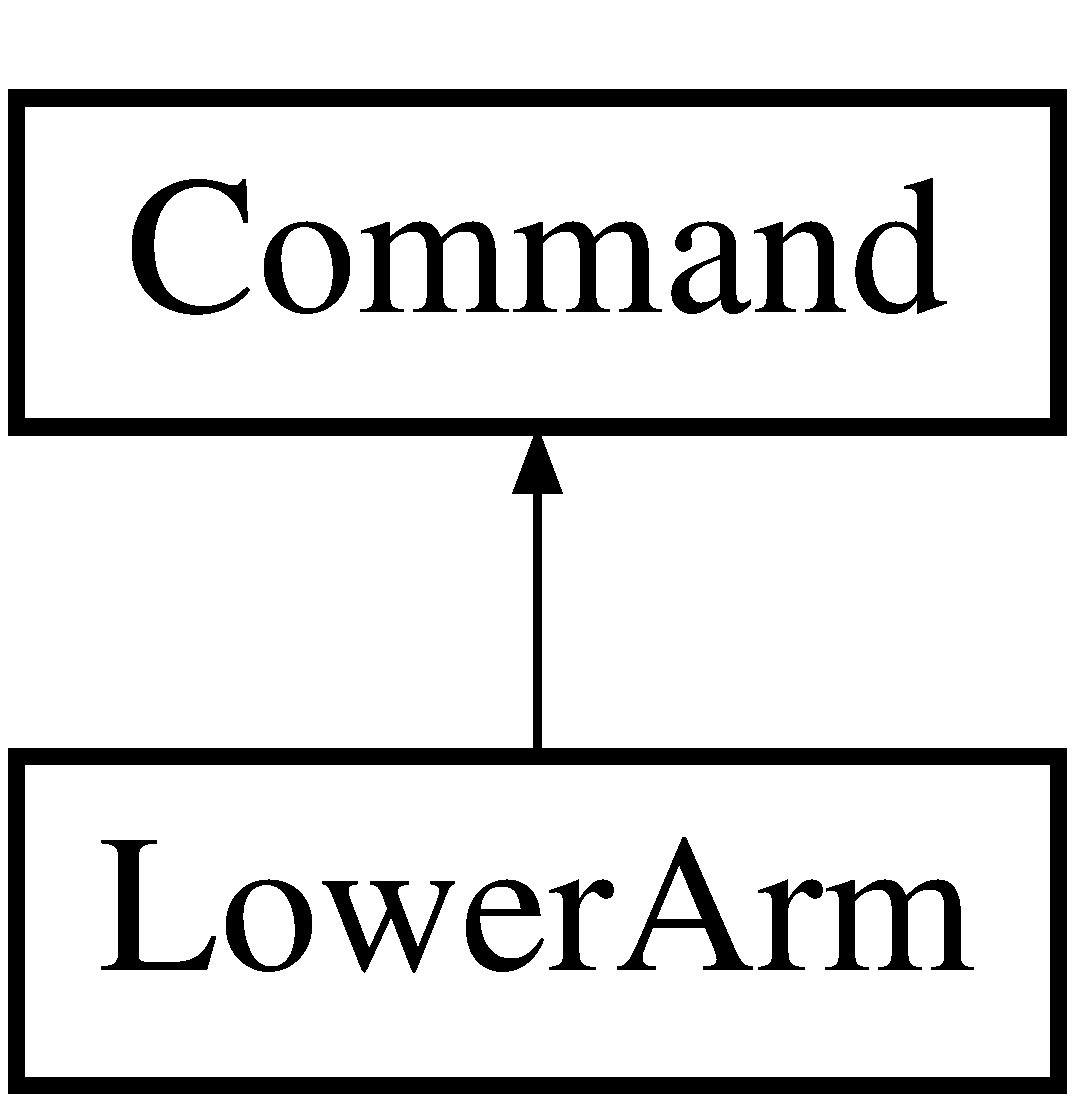
\includegraphics[height=2.000000cm]{classLowerArm}
\end{center}
\end{figure}
\subsection*{Public Member Functions}
\begin{DoxyCompactItemize}
\item 
\hyperlink{classLowerArm_a94252e4c3f22881def50fb2415649f21}{Lower\-Arm} ()
\item 
void \hyperlink{classLowerArm_a4fe99e8f0cdb3526e3847823f69a60b8}{initialize} ()
\begin{DoxyCompactList}\small\item\em run once in the first iteration of the command's life. this will be overrided by individual commands \end{DoxyCompactList}\item 
void \hyperlink{classLowerArm_aca65c2ae64b1ff601213b1ed38ddf8b0}{execute} ()
\begin{DoxyCompactList}\small\item\em stuff to do over and over each iteration. this will be overrided by individual commands \end{DoxyCompactList}\item 
bool \hyperlink{classLowerArm_ad7bb0aadf698f341d737ccefdb015ce2}{is\-Finished} ()
\begin{DoxyCompactList}\small\item\em checked every iteration to see if we're done here. this will be overrided by individual commands \end{DoxyCompactList}\item 
void \hyperlink{classLowerArm_aa46179794b13132a2a353f24c785db37}{end} ()
\begin{DoxyCompactList}\small\item\em called once at the end, once \hyperlink{classLowerArm_ad7bb0aadf698f341d737ccefdb015ce2}{is\-Finished()} returned true. this will be overrided by individual commands. \end{DoxyCompactList}\end{DoxyCompactItemize}
\subsection*{Additional Inherited Members}


\subsection{Detailed Description}


Definition at line 6 of file Lower\-Arm.\-h.



\subsection{Constructor \& Destructor Documentation}
\hypertarget{classLowerArm_a94252e4c3f22881def50fb2415649f21}{\index{Lower\-Arm@{Lower\-Arm}!Lower\-Arm@{Lower\-Arm}}
\index{Lower\-Arm@{Lower\-Arm}!LowerArm@{Lower\-Arm}}
\subsubsection[{Lower\-Arm}]{\setlength{\rightskip}{0pt plus 5cm}Lower\-Arm\-::\-Lower\-Arm (
\begin{DoxyParamCaption}
{}
\end{DoxyParamCaption}
)}}\label{classLowerArm_a94252e4c3f22881def50fb2415649f21}


Definition at line 3 of file Lower\-Arm.\-cpp.



\subsection{Member Function Documentation}
\hypertarget{classLowerArm_aa46179794b13132a2a353f24c785db37}{\index{Lower\-Arm@{Lower\-Arm}!end@{end}}
\index{end@{end}!LowerArm@{Lower\-Arm}}
\subsubsection[{end}]{\setlength{\rightskip}{0pt plus 5cm}void Lower\-Arm\-::end (
\begin{DoxyParamCaption}
{}
\end{DoxyParamCaption}
)\hspace{0.3cm}{\ttfamily [virtual]}}}\label{classLowerArm_aa46179794b13132a2a353f24c785db37}


called once at the end, once \hyperlink{classLowerArm_ad7bb0aadf698f341d737ccefdb015ce2}{is\-Finished()} returned true. this will be overrided by individual commands. 



Implements \hyperlink{classCommand_abed8b7871ba1078bc10056cac5b471be}{Command}.



Definition at line 17 of file Lower\-Arm.\-cpp.

\hypertarget{classLowerArm_aca65c2ae64b1ff601213b1ed38ddf8b0}{\index{Lower\-Arm@{Lower\-Arm}!execute@{execute}}
\index{execute@{execute}!LowerArm@{Lower\-Arm}}
\subsubsection[{execute}]{\setlength{\rightskip}{0pt plus 5cm}void Lower\-Arm\-::execute (
\begin{DoxyParamCaption}
{}
\end{DoxyParamCaption}
)\hspace{0.3cm}{\ttfamily [virtual]}}}\label{classLowerArm_aca65c2ae64b1ff601213b1ed38ddf8b0}


stuff to do over and over each iteration. this will be overrided by individual commands 



Implements \hyperlink{classCommand_a6fd7d9bd8df8bfc881e4d6c7cd1878b7}{Command}.



Definition at line 10 of file Lower\-Arm.\-cpp.

\hypertarget{classLowerArm_a4fe99e8f0cdb3526e3847823f69a60b8}{\index{Lower\-Arm@{Lower\-Arm}!initialize@{initialize}}
\index{initialize@{initialize}!LowerArm@{Lower\-Arm}}
\subsubsection[{initialize}]{\setlength{\rightskip}{0pt plus 5cm}void Lower\-Arm\-::initialize (
\begin{DoxyParamCaption}
{}
\end{DoxyParamCaption}
)\hspace{0.3cm}{\ttfamily [virtual]}}}\label{classLowerArm_a4fe99e8f0cdb3526e3847823f69a60b8}


run once in the first iteration of the command's life. this will be overrided by individual commands 



Implements \hyperlink{classCommand_af186abe582ab15ac64750e4b5d7944de}{Command}.



Definition at line 5 of file Lower\-Arm.\-cpp.

\hypertarget{classLowerArm_ad7bb0aadf698f341d737ccefdb015ce2}{\index{Lower\-Arm@{Lower\-Arm}!is\-Finished@{is\-Finished}}
\index{is\-Finished@{is\-Finished}!LowerArm@{Lower\-Arm}}
\subsubsection[{is\-Finished}]{\setlength{\rightskip}{0pt plus 5cm}bool Lower\-Arm\-::is\-Finished (
\begin{DoxyParamCaption}
{}
\end{DoxyParamCaption}
)\hspace{0.3cm}{\ttfamily [virtual]}}}\label{classLowerArm_ad7bb0aadf698f341d737ccefdb015ce2}


checked every iteration to see if we're done here. this will be overrided by individual commands 

\begin{DoxyReturn}{Returns}
is the function finished 
\end{DoxyReturn}


Implements \hyperlink{classCommand_a9aa704d5f9d98f510a79e645701dc72a}{Command}.



Definition at line 13 of file Lower\-Arm.\-cpp.



The documentation for this class was generated from the following files\-:\begin{DoxyCompactItemize}
\item 
Final\-\_\-\-Project/\hyperlink{LowerArm_8h}{Lower\-Arm.\-h}\item 
Final\-\_\-\-Project/\hyperlink{LowerArm_8cpp}{Lower\-Arm.\-cpp}\end{DoxyCompactItemize}

\hypertarget{classNavigateToAvailableSupply}{\section{Navigate\-To\-Available\-Supply Class Reference}
\label{classNavigateToAvailableSupply}\index{Navigate\-To\-Available\-Supply@{Navigate\-To\-Available\-Supply}}
}
Inheritance diagram for Navigate\-To\-Available\-Supply\-:\begin{figure}[H]
\begin{center}
\leavevmode
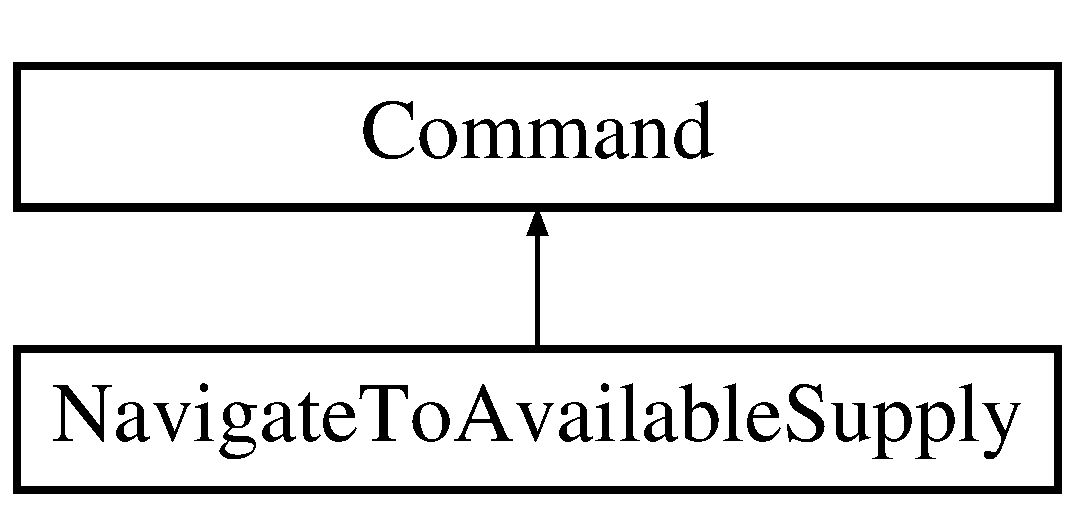
\includegraphics[height=2.000000cm]{classNavigateToAvailableSupply}
\end{center}
\end{figure}
\subsection*{Public Member Functions}
\begin{DoxyCompactItemize}
\item 
\hypertarget{classNavigateToAvailableSupply_a77445727df0f590be945ee6fefe418a0}{void \hyperlink{classNavigateToAvailableSupply_a77445727df0f590be945ee6fefe418a0}{initialize} ()}\label{classNavigateToAvailableSupply_a77445727df0f590be945ee6fefe418a0}

\begin{DoxyCompactList}\small\item\em run once in the first iteration of the command's life. this will be overrided by individual commands \end{DoxyCompactList}\item 
\hypertarget{classNavigateToAvailableSupply_a2c1c22325cc0fa1399530b23ddca7e96}{void \hyperlink{classNavigateToAvailableSupply_a2c1c22325cc0fa1399530b23ddca7e96}{execute} ()}\label{classNavigateToAvailableSupply_a2c1c22325cc0fa1399530b23ddca7e96}

\begin{DoxyCompactList}\small\item\em stuff to do over and over each iteration. this will be overrided by individual commands \end{DoxyCompactList}\item 
bool \hyperlink{classNavigateToAvailableSupply_a7c07bb4eb88b04c835c0b0d27453c43a}{is\-Finished} ()
\begin{DoxyCompactList}\small\item\em checked every iteration to see if we're done here. this will be overrided by individual commands \end{DoxyCompactList}\item 
\hypertarget{classNavigateToAvailableSupply_a92842db484c7f60fe217403783cb8bed}{void \hyperlink{classNavigateToAvailableSupply_a92842db484c7f60fe217403783cb8bed}{end} ()}\label{classNavigateToAvailableSupply_a92842db484c7f60fe217403783cb8bed}

\begin{DoxyCompactList}\small\item\em called once at the end, once \hyperlink{classNavigateToAvailableSupply_a7c07bb4eb88b04c835c0b0d27453c43a}{is\-Finished()} returned true. this will be overrided by individual commands. \end{DoxyCompactList}\end{DoxyCompactItemize}
\subsection*{Additional Inherited Members}


\subsection{Member Function Documentation}
\hypertarget{classNavigateToAvailableSupply_a7c07bb4eb88b04c835c0b0d27453c43a}{\index{Navigate\-To\-Available\-Supply@{Navigate\-To\-Available\-Supply}!is\-Finished@{is\-Finished}}
\index{is\-Finished@{is\-Finished}!NavigateToAvailableSupply@{Navigate\-To\-Available\-Supply}}
\subsubsection[{is\-Finished}]{\setlength{\rightskip}{0pt plus 5cm}bool Navigate\-To\-Available\-Supply\-::is\-Finished (
\begin{DoxyParamCaption}
{}
\end{DoxyParamCaption}
)\hspace{0.3cm}{\ttfamily [virtual]}}}\label{classNavigateToAvailableSupply_a7c07bb4eb88b04c835c0b0d27453c43a}


checked every iteration to see if we're done here. this will be overrided by individual commands 

\begin{DoxyReturn}{Returns}
is the function finished 
\end{DoxyReturn}


Implements \hyperlink{classCommand_a9aa704d5f9d98f510a79e645701dc72a}{Command}.



The documentation for this class was generated from the following files\-:\begin{DoxyCompactItemize}
\item 
Final\-\_\-\-Project/Navigate\-To\-Available\-Supply.\-h\item 
Final\-\_\-\-Project/Navigate\-To\-Available\-Supply.\-cpp\end{DoxyCompactItemize}

\hypertarget{classNavigateToOpenStorage}{\section{Navigate\-To\-Open\-Storage Class Reference}
\label{classNavigateToOpenStorage}\index{Navigate\-To\-Open\-Storage@{Navigate\-To\-Open\-Storage}}
}
Inheritance diagram for Navigate\-To\-Open\-Storage\-:\begin{figure}[H]
\begin{center}
\leavevmode
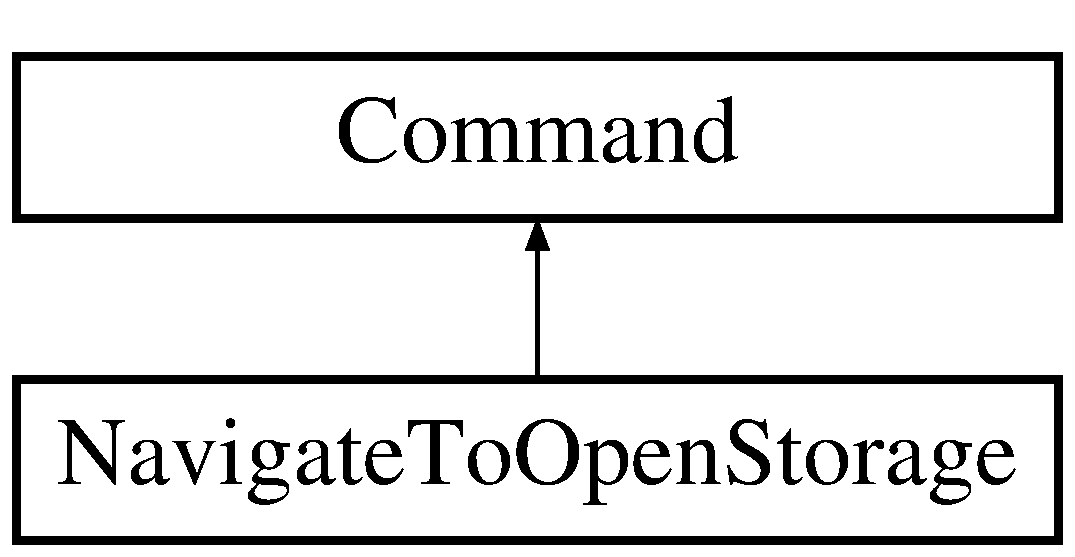
\includegraphics[height=2.000000cm]{classNavigateToOpenStorage}
\end{center}
\end{figure}
\subsection*{Public Member Functions}
\begin{DoxyCompactItemize}
\item 
\hypertarget{classNavigateToOpenStorage_a206ea745d04ffce485b59a7732c932e3}{void \hyperlink{classNavigateToOpenStorage_a206ea745d04ffce485b59a7732c932e3}{initialize} ()}\label{classNavigateToOpenStorage_a206ea745d04ffce485b59a7732c932e3}

\begin{DoxyCompactList}\small\item\em run once in the first iteration of the command's life. this will be overrided by individual commands \end{DoxyCompactList}\item 
\hypertarget{classNavigateToOpenStorage_a12d20167227f6359b0fe95a5d4bd3257}{void \hyperlink{classNavigateToOpenStorage_a12d20167227f6359b0fe95a5d4bd3257}{execute} ()}\label{classNavigateToOpenStorage_a12d20167227f6359b0fe95a5d4bd3257}

\begin{DoxyCompactList}\small\item\em stuff to do over and over each iteration. this will be overrided by individual commands \end{DoxyCompactList}\item 
bool \hyperlink{classNavigateToOpenStorage_ad0b18ef9e40b69bccc01986426e3605c}{is\-Finished} ()
\begin{DoxyCompactList}\small\item\em checked every iteration to see if we're done here. this will be overrided by individual commands \end{DoxyCompactList}\item 
\hypertarget{classNavigateToOpenStorage_af25a3397f1d4aaa94982615fe81f30a2}{void \hyperlink{classNavigateToOpenStorage_af25a3397f1d4aaa94982615fe81f30a2}{end} ()}\label{classNavigateToOpenStorage_af25a3397f1d4aaa94982615fe81f30a2}

\begin{DoxyCompactList}\small\item\em called once at the end, once \hyperlink{classNavigateToOpenStorage_ad0b18ef9e40b69bccc01986426e3605c}{is\-Finished()} returned true. this will be overrided by individual commands. \end{DoxyCompactList}\end{DoxyCompactItemize}
\subsection*{Additional Inherited Members}


\subsection{Member Function Documentation}
\hypertarget{classNavigateToOpenStorage_ad0b18ef9e40b69bccc01986426e3605c}{\index{Navigate\-To\-Open\-Storage@{Navigate\-To\-Open\-Storage}!is\-Finished@{is\-Finished}}
\index{is\-Finished@{is\-Finished}!NavigateToOpenStorage@{Navigate\-To\-Open\-Storage}}
\subsubsection[{is\-Finished}]{\setlength{\rightskip}{0pt plus 5cm}bool Navigate\-To\-Open\-Storage\-::is\-Finished (
\begin{DoxyParamCaption}
{}
\end{DoxyParamCaption}
)\hspace{0.3cm}{\ttfamily [virtual]}}}\label{classNavigateToOpenStorage_ad0b18ef9e40b69bccc01986426e3605c}


checked every iteration to see if we're done here. this will be overrided by individual commands 

\begin{DoxyReturn}{Returns}
is the function finished 
\end{DoxyReturn}


Implements \hyperlink{classCommand_a9aa704d5f9d98f510a79e645701dc72a}{Command}.



The documentation for this class was generated from the following file\-:\begin{DoxyCompactItemize}
\item 
Final\-\_\-\-Project/Navigate\-To\-Open\-Storage.\-h\end{DoxyCompactItemize}

\hypertarget{classNavigateToReactor}{\section{Navigate\-To\-Reactor Class Reference}
\label{classNavigateToReactor}\index{Navigate\-To\-Reactor@{Navigate\-To\-Reactor}}
}
Inheritance diagram for Navigate\-To\-Reactor\-:\begin{figure}[H]
\begin{center}
\leavevmode
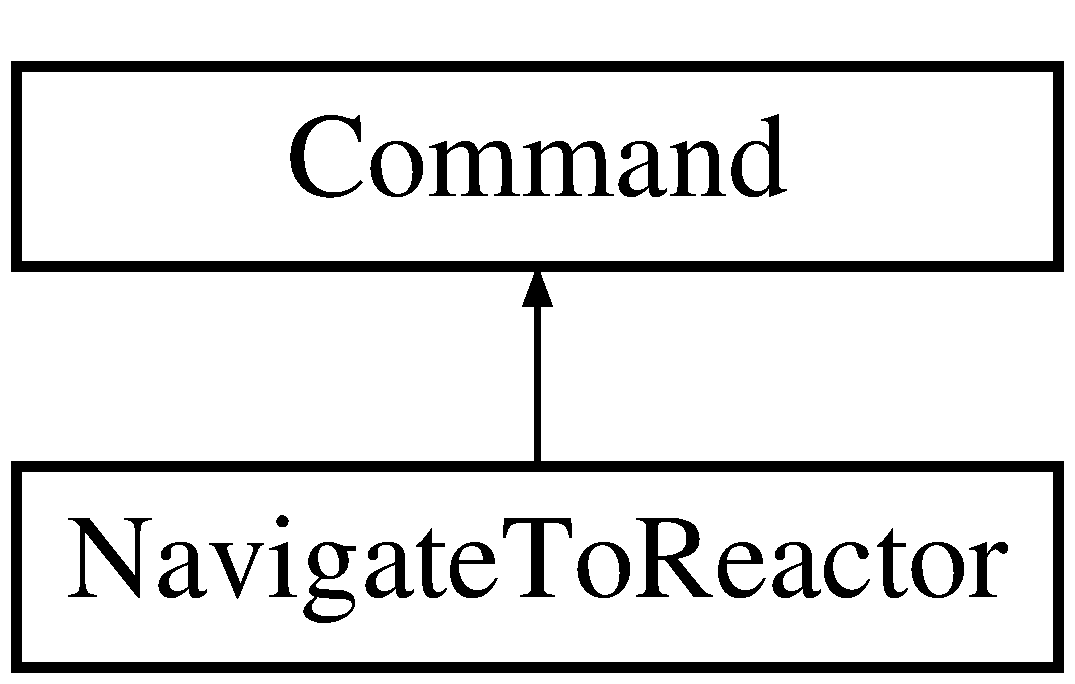
\includegraphics[height=2.000000cm]{classNavigateToReactor}
\end{center}
\end{figure}
\subsection*{Public Member Functions}
\begin{DoxyCompactItemize}
\item 
\hypertarget{classNavigateToReactor_a66a709e79a4c6dc0e7583c9d9a47200d}{{\bfseries Navigate\-To\-Reactor} (int reactor\-Number)}\label{classNavigateToReactor_a66a709e79a4c6dc0e7583c9d9a47200d}

\item 
\hypertarget{classNavigateToReactor_a8b319bd246a3d1c818e38e82ed6ab25f}{void \hyperlink{classNavigateToReactor_a8b319bd246a3d1c818e38e82ed6ab25f}{initialize} ()}\label{classNavigateToReactor_a8b319bd246a3d1c818e38e82ed6ab25f}

\begin{DoxyCompactList}\small\item\em run once in the first iteration of the command's life. this will be overrided by individual commands \end{DoxyCompactList}\item 
\hypertarget{classNavigateToReactor_a50a9743b979ee2a5b35866bbad6f1faa}{void \hyperlink{classNavigateToReactor_a50a9743b979ee2a5b35866bbad6f1faa}{execute} ()}\label{classNavigateToReactor_a50a9743b979ee2a5b35866bbad6f1faa}

\begin{DoxyCompactList}\small\item\em stuff to do over and over each iteration. this will be overrided by individual commands \end{DoxyCompactList}\item 
bool \hyperlink{classNavigateToReactor_ae1619462539af71d2ba9ea167db9dfaf}{is\-Finished} ()
\begin{DoxyCompactList}\small\item\em checked every iteration to see if we're done here. this will be overrided by individual commands \end{DoxyCompactList}\item 
\hypertarget{classNavigateToReactor_a8d42713588dfb661c778ff6aad6c0085}{void \hyperlink{classNavigateToReactor_a8d42713588dfb661c778ff6aad6c0085}{end} ()}\label{classNavigateToReactor_a8d42713588dfb661c778ff6aad6c0085}

\begin{DoxyCompactList}\small\item\em called once at the end, once \hyperlink{classNavigateToReactor_ae1619462539af71d2ba9ea167db9dfaf}{is\-Finished()} returned true. this will be overrided by individual commands. \end{DoxyCompactList}\end{DoxyCompactItemize}
\subsection*{Additional Inherited Members}


\subsection{Member Function Documentation}
\hypertarget{classNavigateToReactor_ae1619462539af71d2ba9ea167db9dfaf}{\index{Navigate\-To\-Reactor@{Navigate\-To\-Reactor}!is\-Finished@{is\-Finished}}
\index{is\-Finished@{is\-Finished}!NavigateToReactor@{Navigate\-To\-Reactor}}
\subsubsection[{is\-Finished}]{\setlength{\rightskip}{0pt plus 5cm}bool Navigate\-To\-Reactor\-::is\-Finished (
\begin{DoxyParamCaption}
{}
\end{DoxyParamCaption}
)\hspace{0.3cm}{\ttfamily [virtual]}}}\label{classNavigateToReactor_ae1619462539af71d2ba9ea167db9dfaf}


checked every iteration to see if we're done here. this will be overrided by individual commands 

\begin{DoxyReturn}{Returns}
is the function finished 
\end{DoxyReturn}


Implements \hyperlink{classCommand_a9aa704d5f9d98f510a79e645701dc72a}{Command}.



The documentation for this class was generated from the following files\-:\begin{DoxyCompactItemize}
\item 
Final\-\_\-\-Project/Navigate\-To\-Reactor.\-h\item 
Final\-\_\-\-Project/Navigate\-To\-Reactor.\-cpp\end{DoxyCompactItemize}

\hypertarget{classOpenGripper}{\section{Open\-Gripper Class Reference}
\label{classOpenGripper}\index{Open\-Gripper@{Open\-Gripper}}
}


{\ttfamily \#include $<$Open\-Gripper.\-h$>$}

Inheritance diagram for Open\-Gripper\-:\begin{figure}[H]
\begin{center}
\leavevmode
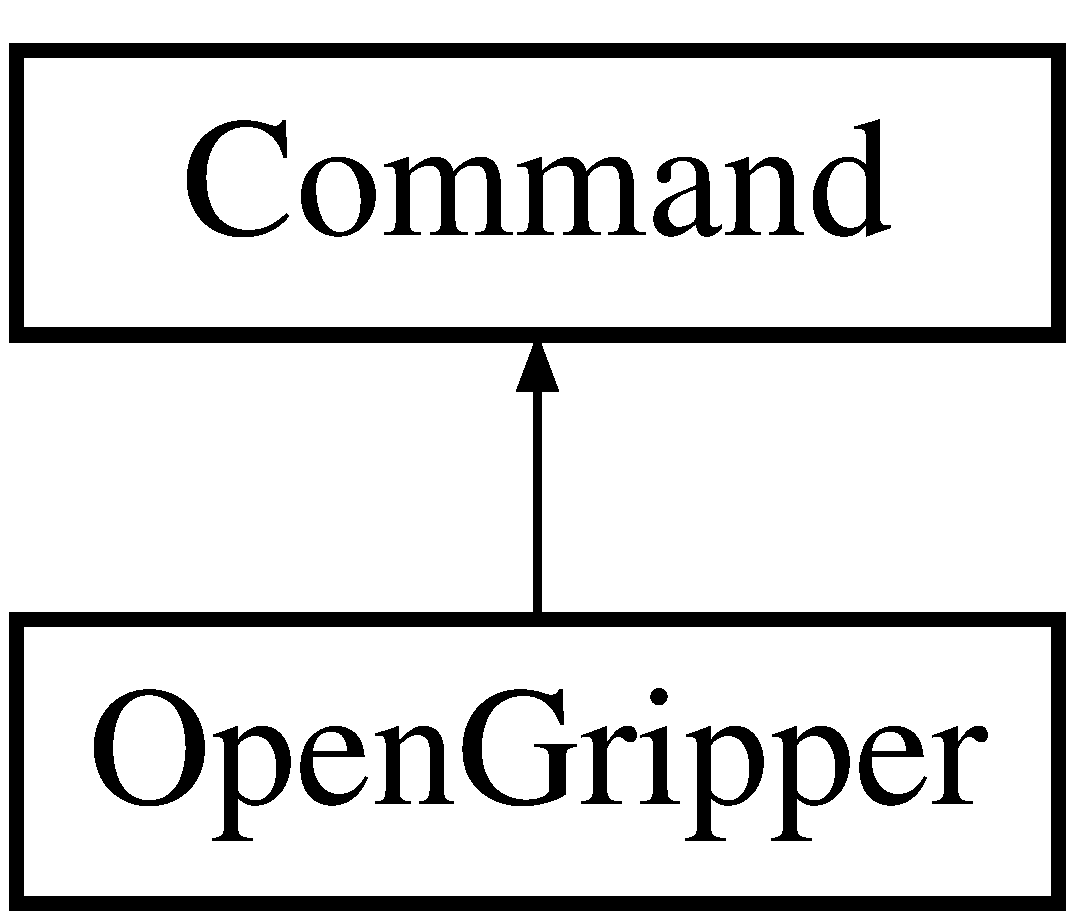
\includegraphics[height=2.000000cm]{classOpenGripper}
\end{center}
\end{figure}
\subsection*{Public Member Functions}
\begin{DoxyCompactItemize}
\item 
\hyperlink{classOpenGripper_af3ca0a56d41c4fbb98e2e5deba76a5a1}{Open\-Gripper} ()
\item 
void \hyperlink{classOpenGripper_a13dc36eb38dc51e85fefbccbef87a981}{initialize} ()
\begin{DoxyCompactList}\small\item\em run once in the first iteration of the command's life. this will be overrided by individual commands \end{DoxyCompactList}\item 
void \hyperlink{classOpenGripper_a358b40de6a9c051a2c7f322747c37dad}{execute} ()
\begin{DoxyCompactList}\small\item\em stuff to do over and over each iteration. this will be overrided by individual commands \end{DoxyCompactList}\item 
bool \hyperlink{classOpenGripper_a334eebec59e348ec33a78d238de85baa}{is\-Finished} ()
\begin{DoxyCompactList}\small\item\em checked every iteration to see if we're done here. this will be overrided by individual commands \end{DoxyCompactList}\item 
void \hyperlink{classOpenGripper_ad807b567e6ca9c8ef0a4f7a143506546}{end} ()
\begin{DoxyCompactList}\small\item\em called once at the end, once \hyperlink{classOpenGripper_a334eebec59e348ec33a78d238de85baa}{is\-Finished()} returned true. this will be overrided by individual commands. \end{DoxyCompactList}\end{DoxyCompactItemize}
\subsection*{Additional Inherited Members}


\subsection{Detailed Description}


Definition at line 6 of file Open\-Gripper.\-h.



\subsection{Constructor \& Destructor Documentation}
\hypertarget{classOpenGripper_af3ca0a56d41c4fbb98e2e5deba76a5a1}{\index{Open\-Gripper@{Open\-Gripper}!Open\-Gripper@{Open\-Gripper}}
\index{Open\-Gripper@{Open\-Gripper}!OpenGripper@{Open\-Gripper}}
\subsubsection[{Open\-Gripper}]{\setlength{\rightskip}{0pt plus 5cm}Open\-Gripper\-::\-Open\-Gripper (
\begin{DoxyParamCaption}
{}
\end{DoxyParamCaption}
)}}\label{classOpenGripper_af3ca0a56d41c4fbb98e2e5deba76a5a1}


Definition at line 3 of file Open\-Gripper.\-cpp.



\subsection{Member Function Documentation}
\hypertarget{classOpenGripper_ad807b567e6ca9c8ef0a4f7a143506546}{\index{Open\-Gripper@{Open\-Gripper}!end@{end}}
\index{end@{end}!OpenGripper@{Open\-Gripper}}
\subsubsection[{end}]{\setlength{\rightskip}{0pt plus 5cm}void Open\-Gripper\-::end (
\begin{DoxyParamCaption}
{}
\end{DoxyParamCaption}
)\hspace{0.3cm}{\ttfamily [virtual]}}}\label{classOpenGripper_ad807b567e6ca9c8ef0a4f7a143506546}


called once at the end, once \hyperlink{classOpenGripper_a334eebec59e348ec33a78d238de85baa}{is\-Finished()} returned true. this will be overrided by individual commands. 



Implements \hyperlink{classCommand_abed8b7871ba1078bc10056cac5b471be}{Command}.



Definition at line 18 of file Open\-Gripper.\-cpp.

\hypertarget{classOpenGripper_a358b40de6a9c051a2c7f322747c37dad}{\index{Open\-Gripper@{Open\-Gripper}!execute@{execute}}
\index{execute@{execute}!OpenGripper@{Open\-Gripper}}
\subsubsection[{execute}]{\setlength{\rightskip}{0pt plus 5cm}void Open\-Gripper\-::execute (
\begin{DoxyParamCaption}
{}
\end{DoxyParamCaption}
)\hspace{0.3cm}{\ttfamily [virtual]}}}\label{classOpenGripper_a358b40de6a9c051a2c7f322747c37dad}


stuff to do over and over each iteration. this will be overrided by individual commands 



Implements \hyperlink{classCommand_a6fd7d9bd8df8bfc881e4d6c7cd1878b7}{Command}.



Definition at line 11 of file Open\-Gripper.\-cpp.

\hypertarget{classOpenGripper_a13dc36eb38dc51e85fefbccbef87a981}{\index{Open\-Gripper@{Open\-Gripper}!initialize@{initialize}}
\index{initialize@{initialize}!OpenGripper@{Open\-Gripper}}
\subsubsection[{initialize}]{\setlength{\rightskip}{0pt plus 5cm}void Open\-Gripper\-::initialize (
\begin{DoxyParamCaption}
{}
\end{DoxyParamCaption}
)\hspace{0.3cm}{\ttfamily [virtual]}}}\label{classOpenGripper_a13dc36eb38dc51e85fefbccbef87a981}


run once in the first iteration of the command's life. this will be overrided by individual commands 



Implements \hyperlink{classCommand_af186abe582ab15ac64750e4b5d7944de}{Command}.



Definition at line 5 of file Open\-Gripper.\-cpp.

\hypertarget{classOpenGripper_a334eebec59e348ec33a78d238de85baa}{\index{Open\-Gripper@{Open\-Gripper}!is\-Finished@{is\-Finished}}
\index{is\-Finished@{is\-Finished}!OpenGripper@{Open\-Gripper}}
\subsubsection[{is\-Finished}]{\setlength{\rightskip}{0pt plus 5cm}bool Open\-Gripper\-::is\-Finished (
\begin{DoxyParamCaption}
{}
\end{DoxyParamCaption}
)\hspace{0.3cm}{\ttfamily [virtual]}}}\label{classOpenGripper_a334eebec59e348ec33a78d238de85baa}


checked every iteration to see if we're done here. this will be overrided by individual commands 

\begin{DoxyReturn}{Returns}
is the function finished 
\end{DoxyReturn}


Implements \hyperlink{classCommand_a9aa704d5f9d98f510a79e645701dc72a}{Command}.



Definition at line 14 of file Open\-Gripper.\-cpp.



The documentation for this class was generated from the following files\-:\begin{DoxyCompactItemize}
\item 
Final\-\_\-\-Project/\hyperlink{OpenGripper_8h}{Open\-Gripper.\-h}\item 
Final\-\_\-\-Project/\hyperlink{OpenGripper_8cpp}{Open\-Gripper.\-cpp}\end{DoxyCompactItemize}

\hypertarget{classPathPlanner}{\section{Path\-Planner Class Reference}
\label{classPathPlanner}\index{Path\-Planner@{Path\-Planner}}
}


Assemble command groups to go from one location to another.  




{\ttfamily \#include $<$Path\-Planner.\-h$>$}

\subsection*{Public Member Functions}
\begin{DoxyCompactItemize}
\item 
\hyperlink{classPathPlanner_a376f30d795cfe0a40f8923f49336f7da}{Path\-Planner} ()
\begin{DoxyCompactList}\small\item\em Constructor. Grabs robot's current position and direction. make sure you call this from the location you want to plan from. \end{DoxyCompactList}\item 
\hyperlink{classCommandGroup}{Command\-Group} $\ast$ \hyperlink{classPathPlanner_acfae981cdde0b63b700bb1e2e9ffc1a6}{plan} (int dest\-Row, int dest\-Col, int dest\-Direction)
\begin{DoxyCompactList}\small\item\em plan from the robot's current position (at time of construction of the plath planner object) to some other point on the field Format is (row,column) 0,0 is the top corner (nothing actually there) 1,0 is the first reactor, (2,2) is storage tube 4, (0,4) is supply tube 1 \end{DoxyCompactList}\end{DoxyCompactItemize}
\subsection*{Static Public Attributes}
\begin{DoxyCompactItemize}
\item 
static const int \hyperlink{classPathPlanner_a701384da34d065d821a936893c5ddd8d}{N\-O\-R\-T\-H} = 0
\begin{DoxyCompactList}\small\item\em convenient constants for navigations \end{DoxyCompactList}\item 
static const int \hyperlink{classPathPlanner_a45399b95a063acdff309e376ccac0fa2}{E\-A\-S\-T} = 1
\item 
static const int \hyperlink{classPathPlanner_a0d74731cd6e012a8724689f8c8f6492e}{S\-O\-U\-T\-H} = 2
\item 
static const int \hyperlink{classPathPlanner_aac8f18908f761050a3801acd476ea0ce}{W\-E\-S\-T} = 3
\item 
static const int \hyperlink{classPathPlanner_af08949a4cd572b26f4f37ff441191b3a}{C\-W} = 1
\item 
static const int \hyperlink{classPathPlanner_ab08a4cb0f762a4401a804bf0ce1bbbe6}{C\-C\-W} = -\/1
\end{DoxyCompactItemize}
\subsection*{Private Member Functions}
\begin{DoxyCompactItemize}
\item 
void \hyperlink{classPathPlanner_a435470288f6e2b5f99ce590db0bfc5db}{plan\-To\-Face} (int current\-Direction)
\begin{DoxyCompactList}\small\item\em adds command groups to the path for turning \end{DoxyCompactList}\end{DoxyCompactItemize}
\subsection*{Private Attributes}
\begin{DoxyCompactItemize}
\item 
int \hyperlink{classPathPlanner_a20d2bf800c63aacfd1af314ad400d119}{col}
\begin{DoxyCompactList}\small\item\em ints for storing current col row and direction in the plan \end{DoxyCompactList}\item 
int \hyperlink{classPathPlanner_a00b0fa8525a5fe9c8088ccaa005c4c54}{row}
\item 
int \hyperlink{classPathPlanner_a1f9985b79ca49ca0b2992176a10a6210}{direction}
\item 
\hyperlink{classCommandGroup}{Command\-Group} $\ast$ \hyperlink{classPathPlanner_a9b41e5ee68a78a45e46003102a6c3b91}{path}
\begin{DoxyCompactList}\small\item\em \hyperlink{classCommandGroup}{Command\-Group} to be assembled. \end{DoxyCompactList}\end{DoxyCompactItemize}


\subsection{Detailed Description}
Assemble command groups to go from one location to another. 

Definition at line 4 of file Path\-Planner.\-h.



\subsection{Constructor \& Destructor Documentation}
\hypertarget{classPathPlanner_a376f30d795cfe0a40f8923f49336f7da}{\index{Path\-Planner@{Path\-Planner}!Path\-Planner@{Path\-Planner}}
\index{Path\-Planner@{Path\-Planner}!PathPlanner@{Path\-Planner}}
\subsubsection[{Path\-Planner}]{\setlength{\rightskip}{0pt plus 5cm}Path\-Planner\-::\-Path\-Planner (
\begin{DoxyParamCaption}
{}
\end{DoxyParamCaption}
)}}\label{classPathPlanner_a376f30d795cfe0a40f8923f49336f7da}


Constructor. Grabs robot's current position and direction. make sure you call this from the location you want to plan from. 



Definition at line 9 of file Path\-Planner.\-cpp.



\subsection{Member Function Documentation}
\hypertarget{classPathPlanner_acfae981cdde0b63b700bb1e2e9ffc1a6}{\index{Path\-Planner@{Path\-Planner}!plan@{plan}}
\index{plan@{plan}!PathPlanner@{Path\-Planner}}
\subsubsection[{plan}]{\setlength{\rightskip}{0pt plus 5cm}{\bf Command\-Group} $\ast$ Path\-Planner\-::plan (
\begin{DoxyParamCaption}
\item[{int}]{dest\-Row, }
\item[{int}]{dest\-Col, }
\item[{int}]{dest\-Direction}
\end{DoxyParamCaption}
)}}\label{classPathPlanner_acfae981cdde0b63b700bb1e2e9ffc1a6}


plan from the robot's current position (at time of construction of the plath planner object) to some other point on the field Format is (row,column) 0,0 is the top corner (nothing actually there) 1,0 is the first reactor, (2,2) is storage tube 4, (0,4) is supply tube 1 



Definition at line 16 of file Path\-Planner.\-cpp.

\hypertarget{classPathPlanner_a435470288f6e2b5f99ce590db0bfc5db}{\index{Path\-Planner@{Path\-Planner}!plan\-To\-Face@{plan\-To\-Face}}
\index{plan\-To\-Face@{plan\-To\-Face}!PathPlanner@{Path\-Planner}}
\subsubsection[{plan\-To\-Face}]{\setlength{\rightskip}{0pt plus 5cm}void Path\-Planner\-::plan\-To\-Face (
\begin{DoxyParamCaption}
\item[{int}]{current\-Direction}
\end{DoxyParamCaption}
)\hspace{0.3cm}{\ttfamily [private]}}}\label{classPathPlanner_a435470288f6e2b5f99ce590db0bfc5db}


adds command groups to the path for turning 


\begin{DoxyParams}{Parameters}
{\em \-\_\-in\mbox{]}} & current\-Direction the direction you're facing at this point in the plan \\
\hline
\end{DoxyParams}


Definition at line 87 of file Path\-Planner.\-cpp.



\subsection{Member Data Documentation}
\hypertarget{classPathPlanner_ab08a4cb0f762a4401a804bf0ce1bbbe6}{\index{Path\-Planner@{Path\-Planner}!C\-C\-W@{C\-C\-W}}
\index{C\-C\-W@{C\-C\-W}!PathPlanner@{Path\-Planner}}
\subsubsection[{C\-C\-W}]{\setlength{\rightskip}{0pt plus 5cm}const int Path\-Planner\-::\-C\-C\-W = -\/1\hspace{0.3cm}{\ttfamily [static]}}}\label{classPathPlanner_ab08a4cb0f762a4401a804bf0ce1bbbe6}


Definition at line 26 of file Path\-Planner.\-h.

\hypertarget{classPathPlanner_a20d2bf800c63aacfd1af314ad400d119}{\index{Path\-Planner@{Path\-Planner}!col@{col}}
\index{col@{col}!PathPlanner@{Path\-Planner}}
\subsubsection[{col}]{\setlength{\rightskip}{0pt plus 5cm}int Path\-Planner\-::col\hspace{0.3cm}{\ttfamily [private]}}}\label{classPathPlanner_a20d2bf800c63aacfd1af314ad400d119}


ints for storing current col row and direction in the plan 



Definition at line 36 of file Path\-Planner.\-h.

\hypertarget{classPathPlanner_af08949a4cd572b26f4f37ff441191b3a}{\index{Path\-Planner@{Path\-Planner}!C\-W@{C\-W}}
\index{C\-W@{C\-W}!PathPlanner@{Path\-Planner}}
\subsubsection[{C\-W}]{\setlength{\rightskip}{0pt plus 5cm}const int Path\-Planner\-::\-C\-W = 1\hspace{0.3cm}{\ttfamily [static]}}}\label{classPathPlanner_af08949a4cd572b26f4f37ff441191b3a}


Definition at line 25 of file Path\-Planner.\-h.

\hypertarget{classPathPlanner_a1f9985b79ca49ca0b2992176a10a6210}{\index{Path\-Planner@{Path\-Planner}!direction@{direction}}
\index{direction@{direction}!PathPlanner@{Path\-Planner}}
\subsubsection[{direction}]{\setlength{\rightskip}{0pt plus 5cm}int Path\-Planner\-::direction\hspace{0.3cm}{\ttfamily [private]}}}\label{classPathPlanner_a1f9985b79ca49ca0b2992176a10a6210}


Definition at line 36 of file Path\-Planner.\-h.

\hypertarget{classPathPlanner_a45399b95a063acdff309e376ccac0fa2}{\index{Path\-Planner@{Path\-Planner}!E\-A\-S\-T@{E\-A\-S\-T}}
\index{E\-A\-S\-T@{E\-A\-S\-T}!PathPlanner@{Path\-Planner}}
\subsubsection[{E\-A\-S\-T}]{\setlength{\rightskip}{0pt plus 5cm}const int Path\-Planner\-::\-E\-A\-S\-T = 1\hspace{0.3cm}{\ttfamily [static]}}}\label{classPathPlanner_a45399b95a063acdff309e376ccac0fa2}


Definition at line 22 of file Path\-Planner.\-h.

\hypertarget{classPathPlanner_a701384da34d065d821a936893c5ddd8d}{\index{Path\-Planner@{Path\-Planner}!N\-O\-R\-T\-H@{N\-O\-R\-T\-H}}
\index{N\-O\-R\-T\-H@{N\-O\-R\-T\-H}!PathPlanner@{Path\-Planner}}
\subsubsection[{N\-O\-R\-T\-H}]{\setlength{\rightskip}{0pt plus 5cm}const int Path\-Planner\-::\-N\-O\-R\-T\-H = 0\hspace{0.3cm}{\ttfamily [static]}}}\label{classPathPlanner_a701384da34d065d821a936893c5ddd8d}


convenient constants for navigations 



Definition at line 21 of file Path\-Planner.\-h.

\hypertarget{classPathPlanner_a9b41e5ee68a78a45e46003102a6c3b91}{\index{Path\-Planner@{Path\-Planner}!path@{path}}
\index{path@{path}!PathPlanner@{Path\-Planner}}
\subsubsection[{path}]{\setlength{\rightskip}{0pt plus 5cm}{\bf Command\-Group}$\ast$ Path\-Planner\-::path\hspace{0.3cm}{\ttfamily [private]}}}\label{classPathPlanner_a9b41e5ee68a78a45e46003102a6c3b91}


\hyperlink{classCommandGroup}{Command\-Group} to be assembled. 



Definition at line 39 of file Path\-Planner.\-h.

\hypertarget{classPathPlanner_a00b0fa8525a5fe9c8088ccaa005c4c54}{\index{Path\-Planner@{Path\-Planner}!row@{row}}
\index{row@{row}!PathPlanner@{Path\-Planner}}
\subsubsection[{row}]{\setlength{\rightskip}{0pt plus 5cm}int Path\-Planner\-::row\hspace{0.3cm}{\ttfamily [private]}}}\label{classPathPlanner_a00b0fa8525a5fe9c8088ccaa005c4c54}


Definition at line 36 of file Path\-Planner.\-h.

\hypertarget{classPathPlanner_a0d74731cd6e012a8724689f8c8f6492e}{\index{Path\-Planner@{Path\-Planner}!S\-O\-U\-T\-H@{S\-O\-U\-T\-H}}
\index{S\-O\-U\-T\-H@{S\-O\-U\-T\-H}!PathPlanner@{Path\-Planner}}
\subsubsection[{S\-O\-U\-T\-H}]{\setlength{\rightskip}{0pt plus 5cm}const int Path\-Planner\-::\-S\-O\-U\-T\-H = 2\hspace{0.3cm}{\ttfamily [static]}}}\label{classPathPlanner_a0d74731cd6e012a8724689f8c8f6492e}


Definition at line 23 of file Path\-Planner.\-h.

\hypertarget{classPathPlanner_aac8f18908f761050a3801acd476ea0ce}{\index{Path\-Planner@{Path\-Planner}!W\-E\-S\-T@{W\-E\-S\-T}}
\index{W\-E\-S\-T@{W\-E\-S\-T}!PathPlanner@{Path\-Planner}}
\subsubsection[{W\-E\-S\-T}]{\setlength{\rightskip}{0pt plus 5cm}const int Path\-Planner\-::\-W\-E\-S\-T = 3\hspace{0.3cm}{\ttfamily [static]}}}\label{classPathPlanner_aac8f18908f761050a3801acd476ea0ce}


Definition at line 24 of file Path\-Planner.\-h.



The documentation for this class was generated from the following files\-:\begin{DoxyCompactItemize}
\item 
Final\-\_\-\-Project/\hyperlink{PathPlanner_8h}{Path\-Planner.\-h}\item 
Final\-\_\-\-Project/\hyperlink{PathPlanner_8cpp}{Path\-Planner.\-cpp}\end{DoxyCompactItemize}

\hypertarget{classRaiseArm}{\section{Raise\-Arm Class Reference}
\label{classRaiseArm}\index{Raise\-Arm@{Raise\-Arm}}
}


{\ttfamily \#include $<$Raise\-Arm.\-h$>$}

Inheritance diagram for Raise\-Arm\-:\begin{figure}[H]
\begin{center}
\leavevmode
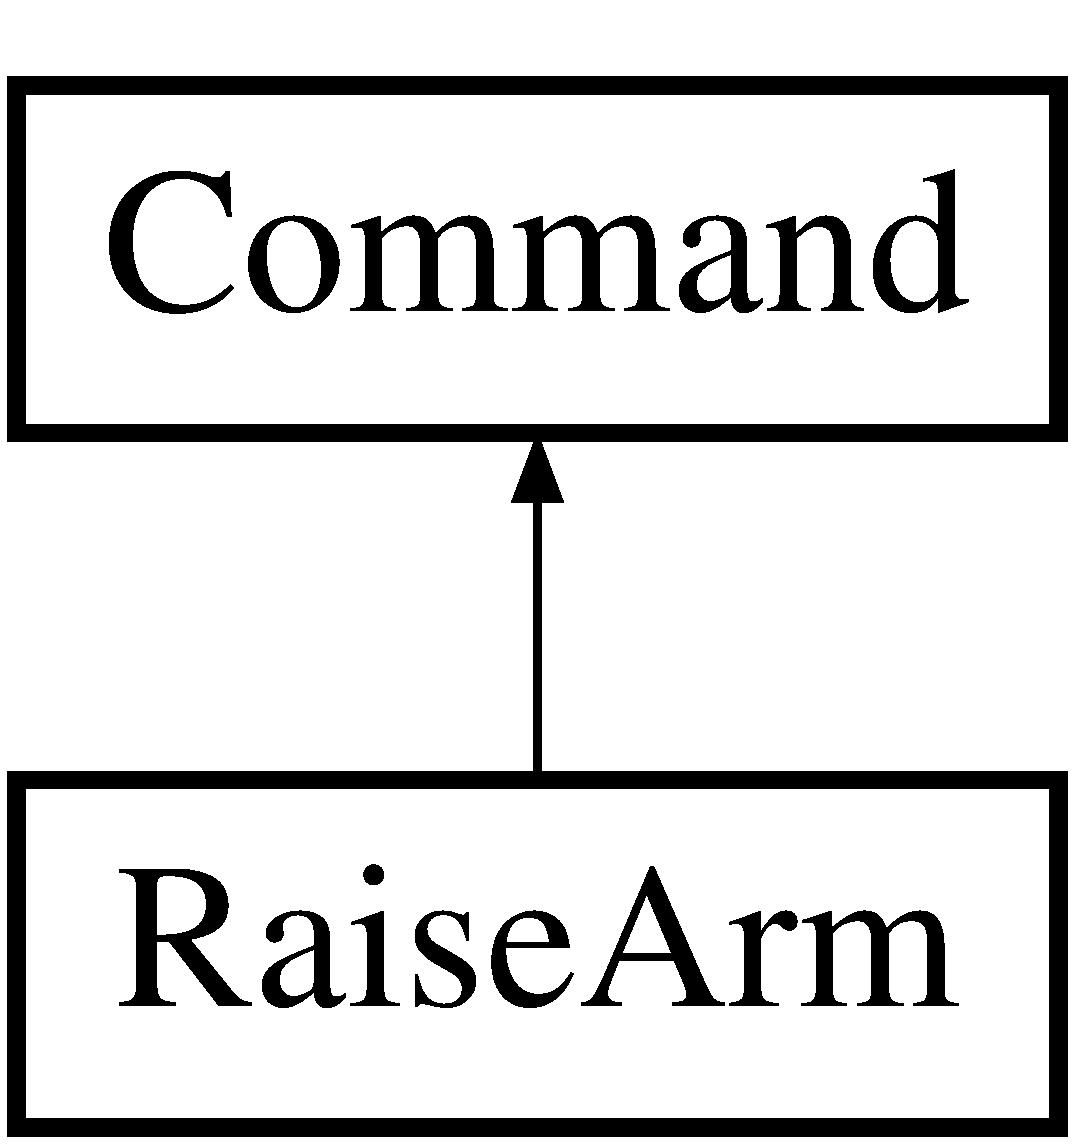
\includegraphics[height=2.000000cm]{classRaiseArm}
\end{center}
\end{figure}
\subsection*{Public Member Functions}
\begin{DoxyCompactItemize}
\item 
\hyperlink{classRaiseArm_a91b62d0ce0bae3391a2fdb617b603f8b}{Raise\-Arm} ()
\item 
void \hyperlink{classRaiseArm_a643abff446802bf06eb0141d3cad5ef4}{initialize} ()
\begin{DoxyCompactList}\small\item\em run once in the first iteration of the command's life. this will be overrided by individual commands \end{DoxyCompactList}\item 
void \hyperlink{classRaiseArm_a4e73ea27587532325bfea84e2fe72f62}{execute} ()
\begin{DoxyCompactList}\small\item\em stuff to do over and over each iteration. this will be overrided by individual commands \end{DoxyCompactList}\item 
bool \hyperlink{classRaiseArm_a3f2f2806c7b255589864feae9322bbd1}{is\-Finished} ()
\begin{DoxyCompactList}\small\item\em checked every iteration to see if we're done here. this will be overrided by individual commands \end{DoxyCompactList}\item 
void \hyperlink{classRaiseArm_a61c556ef1ca7e8c92970cec3baef933e}{end} ()
\begin{DoxyCompactList}\small\item\em called once at the end, once \hyperlink{classRaiseArm_a3f2f2806c7b255589864feae9322bbd1}{is\-Finished()} returned true. this will be overrided by individual commands. \end{DoxyCompactList}\end{DoxyCompactItemize}
\subsection*{Additional Inherited Members}


\subsection{Detailed Description}


Definition at line 6 of file Raise\-Arm.\-h.



\subsection{Constructor \& Destructor Documentation}
\hypertarget{classRaiseArm_a91b62d0ce0bae3391a2fdb617b603f8b}{\index{Raise\-Arm@{Raise\-Arm}!Raise\-Arm@{Raise\-Arm}}
\index{Raise\-Arm@{Raise\-Arm}!RaiseArm@{Raise\-Arm}}
\subsubsection[{Raise\-Arm}]{\setlength{\rightskip}{0pt plus 5cm}Raise\-Arm\-::\-Raise\-Arm (
\begin{DoxyParamCaption}
{}
\end{DoxyParamCaption}
)}}\label{classRaiseArm_a91b62d0ce0bae3391a2fdb617b603f8b}


Definition at line 3 of file Raise\-Arm.\-cpp.



\subsection{Member Function Documentation}
\hypertarget{classRaiseArm_a61c556ef1ca7e8c92970cec3baef933e}{\index{Raise\-Arm@{Raise\-Arm}!end@{end}}
\index{end@{end}!RaiseArm@{Raise\-Arm}}
\subsubsection[{end}]{\setlength{\rightskip}{0pt plus 5cm}void Raise\-Arm\-::end (
\begin{DoxyParamCaption}
{}
\end{DoxyParamCaption}
)\hspace{0.3cm}{\ttfamily [virtual]}}}\label{classRaiseArm_a61c556ef1ca7e8c92970cec3baef933e}


called once at the end, once \hyperlink{classRaiseArm_a3f2f2806c7b255589864feae9322bbd1}{is\-Finished()} returned true. this will be overrided by individual commands. 



Implements \hyperlink{classCommand_abed8b7871ba1078bc10056cac5b471be}{Command}.



Definition at line 16 of file Raise\-Arm.\-cpp.

\hypertarget{classRaiseArm_a4e73ea27587532325bfea84e2fe72f62}{\index{Raise\-Arm@{Raise\-Arm}!execute@{execute}}
\index{execute@{execute}!RaiseArm@{Raise\-Arm}}
\subsubsection[{execute}]{\setlength{\rightskip}{0pt plus 5cm}void Raise\-Arm\-::execute (
\begin{DoxyParamCaption}
{}
\end{DoxyParamCaption}
)\hspace{0.3cm}{\ttfamily [virtual]}}}\label{classRaiseArm_a4e73ea27587532325bfea84e2fe72f62}


stuff to do over and over each iteration. this will be overrided by individual commands 



Implements \hyperlink{classCommand_a6fd7d9bd8df8bfc881e4d6c7cd1878b7}{Command}.



Definition at line 10 of file Raise\-Arm.\-cpp.

\hypertarget{classRaiseArm_a643abff446802bf06eb0141d3cad5ef4}{\index{Raise\-Arm@{Raise\-Arm}!initialize@{initialize}}
\index{initialize@{initialize}!RaiseArm@{Raise\-Arm}}
\subsubsection[{initialize}]{\setlength{\rightskip}{0pt plus 5cm}void Raise\-Arm\-::initialize (
\begin{DoxyParamCaption}
{}
\end{DoxyParamCaption}
)\hspace{0.3cm}{\ttfamily [virtual]}}}\label{classRaiseArm_a643abff446802bf06eb0141d3cad5ef4}


run once in the first iteration of the command's life. this will be overrided by individual commands 



Implements \hyperlink{classCommand_af186abe582ab15ac64750e4b5d7944de}{Command}.



Definition at line 5 of file Raise\-Arm.\-cpp.

\hypertarget{classRaiseArm_a3f2f2806c7b255589864feae9322bbd1}{\index{Raise\-Arm@{Raise\-Arm}!is\-Finished@{is\-Finished}}
\index{is\-Finished@{is\-Finished}!RaiseArm@{Raise\-Arm}}
\subsubsection[{is\-Finished}]{\setlength{\rightskip}{0pt plus 5cm}bool Raise\-Arm\-::is\-Finished (
\begin{DoxyParamCaption}
{}
\end{DoxyParamCaption}
)\hspace{0.3cm}{\ttfamily [virtual]}}}\label{classRaiseArm_a3f2f2806c7b255589864feae9322bbd1}


checked every iteration to see if we're done here. this will be overrided by individual commands 

\begin{DoxyReturn}{Returns}
is the function finished 
\end{DoxyReturn}


Implements \hyperlink{classCommand_a9aa704d5f9d98f510a79e645701dc72a}{Command}.



Definition at line 12 of file Raise\-Arm.\-cpp.



The documentation for this class was generated from the following files\-:\begin{DoxyCompactItemize}
\item 
Final\-\_\-\-Project/\hyperlink{RaiseArm_8h}{Raise\-Arm.\-h}\item 
Final\-\_\-\-Project/\hyperlink{RaiseArm_8cpp}{Raise\-Arm.\-cpp}\end{DoxyCompactItemize}

\hypertarget{classRobot}{\section{Robot Class Reference}
\label{classRobot}\index{Robot@{Robot}}
}


functions here control the robot as a whole. leds, bluetooth, arm, and line sensor, and music are immediate components.  




{\ttfamily \#include $<$Robot.\-h$>$}

\subsection*{Public Member Functions}
\begin{DoxyCompactItemize}
\item 
void \hyperlink{classRobot_a1fc37e3c329d59795f6adf44199d4df9}{setup} ()
\begin{DoxyCompactList}\small\item\em lsetup servos and stuff. called by main setup \end{DoxyCompactList}\item 
void \hyperlink{classRobot_a4215f7e880311c2118f387df75effaf2}{blink\-L\-E\-Ds} ()
\begin{DoxyCompactList}\small\item\em inidicate radiation by blinking L\-E\-Ds every 1/5th of a second \end{DoxyCompactList}\item 
void \hyperlink{classRobot_a87e94e8db5092976d1125c674cf2b519}{set\-Song} (int track\-Number, bool repeat)
\begin{DoxyCompactList}\small\item\em sends correct int over i2c to slave to play song. Simple protocol is used to encode song data. If the first bit is 1, the song will repeat. All other bits are for the song number \end{DoxyCompactList}\item 
void \hyperlink{classRobot_ad86dbbb2ad0d065f3e4c30fd4b742e1c}{play\-Song} ()
\begin{DoxyCompactList}\small\item\em sends the encoded data over i2c to the slave \end{DoxyCompactList}\item 
void \hyperlink{classRobot_a7c4cf197187f9f7dcb883ebc58f52b93}{pause\-Song} ()
\begin{DoxyCompactList}\small\item\em sends correct int over i2c to slave to plause song \end{DoxyCompactList}\item 
void \hyperlink{classRobot_a6e3caf6e0346f6a54557eb57a79fc4f4}{follow\-Line} ()
\begin{DoxyCompactList}\small\item\em uses line sensor to follow line following is done by a weighted power to each wheel weight is a function of the intensity of line sensors on that side low intensity -\/$>$ white -\/$>$ full motor power high intensity -\/$>$ black -\/$>$ full reverse motor power \end{DoxyCompactList}\item 
void \hyperlink{classRobot_a450cf38f963596663003f3d94b2bcf3b}{back\-Up} (int r\-Power, int l\-Power)
\begin{DoxyCompactList}\small\item\em blindly back up \end{DoxyCompactList}\item 
void \hyperlink{classRobot_a959f64b4829ade78bb332f205b50ee70}{stop\-Driving} ()
\begin{DoxyCompactList}\small\item\em stop driving \end{DoxyCompactList}\item 
void \hyperlink{classRobot_a35897f5e7b5c8b29cc6d386c6089abea}{drive\-Fwd} ()
\begin{DoxyCompactList}\small\item\em forward drive no line track \end{DoxyCompactList}\item 
void \hyperlink{classRobot_ac8d0a3e0308350bc1fc3a2a78be2aaca}{drive\-Bwd} ()
\begin{DoxyCompactList}\small\item\em backward drive \end{DoxyCompactList}\item 
void \hyperlink{classRobot_a82a61a1f5fb4a17fd2277329bc6e8fe4}{rotate\-Left} ()
\begin{DoxyCompactList}\small\item\em fixed power rotate \end{DoxyCompactList}\item 
void \hyperlink{classRobot_a33e931c5ce2e2ce940c96203f1b6d057}{rotate\-Right} ()
\begin{DoxyCompactList}\small\item\em fixed power rotate \end{DoxyCompactList}\item 
bool \hyperlink{classRobot_a9183b1dd60c7d39bf6c8ecea5690b22c}{at\-Reactor\-Tube} ()
\begin{DoxyCompactList}\small\item\em check is we've hit a reactor tube \end{DoxyCompactList}\item 
void \hyperlink{classRobot_ab7c87529c987ede12b934bdfc768507e}{reset\-Timer\-Flags} ()
\begin{DoxyCompactList}\small\item\em sets all timer flags to false \end{DoxyCompactList}\end{DoxyCompactItemize}
\subsection*{Static Public Member Functions}
\begin{DoxyCompactItemize}
\item 
static \hyperlink{classRobot}{Robot} $\ast$ \hyperlink{classRobot_ac6f19dc31b435f8a2d43944ba49286d0}{get\-Instance} ()
\begin{DoxyCompactList}\small\item\em lsingle accesor \end{DoxyCompactList}\end{DoxyCompactItemize}
\subsection*{Public Attributes}
\begin{DoxyCompactItemize}
\item 
int \hyperlink{classRobot_a35ce5c416a079fcf6b943843ec151d63}{row}
\begin{DoxyCompactList}\small\item\em used to store position updated by navigate commands should only be checked when the robot is done moving direction is as follow\-: N=0, E=1, S=2, W=3 \end{DoxyCompactList}\item 
int \hyperlink{classRobot_a2e08d53491bb82defe2e28ee9ce1d096}{col}
\item 
int \hyperlink{classRobot_ac25b4dfc2e9e5aa86ec5684d075d32b8}{direction}
\item 
\hyperlink{classBTClient}{B\-T\-Client} \hyperlink{classRobot_a9da91e6d551ed02038e935b3c755cc75}{bt\-Client}
\begin{DoxyCompactList}\small\item\em the object for reading and sending bluetooth message \end{DoxyCompactList}\item 
\hyperlink{classArm}{Arm} \hyperlink{classRobot_a444673862cbe384992aceb066282b500}{arm}
\begin{DoxyCompactList}\small\item\em the object for controling the arm \end{DoxyCompactList}\item 
\hyperlink{classLineSensor}{Line\-Sensor} \hyperlink{classRobot_abdc300045bea9a31013b25682629752d}{line\-Sensor}
\begin{DoxyCompactList}\small\item\em the object for tracking position over the lines \end{DoxyCompactList}\item 
bool \hyperlink{classRobot_a6a1fae6e6ee0a3298b9e60d3f50ad12a}{paused}
\begin{DoxyCompactList}\small\item\em set by bluetooth if resume/stop message is recieve all drive motor commands depend on it being true \end{DoxyCompactList}\item 
bool \hyperlink{classRobot_a77f62d85ab1cf34e79c2a3acd470a4ce}{radiating} = false
\begin{DoxyCompactList}\small\item\em flag for blinking L\-E\-Ds based on radiaiton to turn off L\-E\-Ds, set this to false \end{DoxyCompactList}\end{DoxyCompactItemize}
\subsection*{Static Public Attributes}
\begin{DoxyCompactItemize}
\item 
static const int \hyperlink{classRobot_ac40abfa06749a68604af90c00e2a3fee}{C\-A\-L\-I\-B\-R\-A\-T\-E\-\_\-\-T\-I\-M\-E} = 3000
\end{DoxyCompactItemize}
\subsection*{Private Member Functions}
\begin{DoxyCompactItemize}
\item 
\hyperlink{classRobot_a4fc7c70ae20623f05e06f2ecb388b6c4}{Robot} ()
\begin{DoxyCompactList}\small\item\em there's only one robot, so use private constructor and instance \end{DoxyCompactList}\item 
void \hyperlink{classRobot_aad8723ec56e9fc8ca17da5ef79de37d6}{drive} (int left\-Power, int right\-Power)
\begin{DoxyCompactList}\small\item\em low level function for setting motor power input is limited between -\/100 (full back) and 100 (full forward) \end{DoxyCompactList}\end{DoxyCompactItemize}
\subsection*{Static Private Member Functions}
\begin{DoxyCompactItemize}
\item 
static void \hyperlink{classRobot_a9908dfe5a06008e6203edca94d30327a}{pause} ()
\begin{DoxyCompactList}\small\item\em lused by bumper switch as a panic button function \end{DoxyCompactList}\item 
static void \hyperlink{classRobot_afb5418d31b61a64e0930fd1fb495c8c9}{blink\-And\-Send\-Interrupt} ()
\begin{DoxyCompactList}\small\item\em interrupt changes state of L\-E\-D blink and send i2c \end{DoxyCompactList}\end{DoxyCompactItemize}
\subsection*{Private Attributes}
\begin{DoxyCompactItemize}
\item 
Servo \hyperlink{classRobot_af357e059c6c07190c92c6c9a00e2b8af}{left\-Wheel}
\begin{DoxyCompactList}\small\item\em drive wheels \end{DoxyCompactList}\item 
Servo \hyperlink{classRobot_a3b2dd5b89e44fd3a7ba239554fb5b8a7}{right\-Wheel}
\item 
int \hyperlink{classRobot_a3c7308c71db125a8840f9c82b5fec9ca}{led\-State}
\begin{DoxyCompactList}\small\item\em controls state of led when radiating \end{DoxyCompactList}\item 
int \hyperlink{classRobot_a7818916adfa736ab4cb21011fe302cdb}{song\-Data}
\begin{DoxyCompactList}\small\item\em the encoded data to send over i2\-C \end{DoxyCompactList}\item 
const int \hyperlink{classRobot_a351d754436c8f569432ef7a06641f98a}{reactor\-Tube\-Limit\-Pin} = 28
\item 
const int \hyperlink{classRobot_a4063d601b5b4d5aad332f617abb36c7b}{rotate\-Speed} = 28
\item 
const int \hyperlink{classRobot_a87ec942d7d53b1a4b1c46422f6a134eb}{travel\-Speed} = 26
\end{DoxyCompactItemize}
\subsection*{Static Private Attributes}
\begin{DoxyCompactItemize}
\item 
static \hyperlink{classRobot}{Robot} $\ast$ \hyperlink{classRobot_aad5c5d6db601aac62393d47ec9385fa3}{instance} = N\-U\-L\-L
\item 
static bool \hyperlink{classRobot_aa074884ad594acf20282805c811adaff}{time\-To\-Blink\-And\-Send} = false
\begin{DoxyCompactList}\small\item\em set by led timer interrupt \end{DoxyCompactList}\item 
static const int \hyperlink{classRobot_a431ea8916b52ddfddbe6d80a09fe71e0}{L\-E\-D\-\_\-\-P\-I\-N0} = 22
\item 
static const int \hyperlink{classRobot_a4c6f4e38b77bf470d757ebea1b8c3cf0}{L\-E\-D\-\_\-\-P\-I\-N1} = 23
\item 
static const int \hyperlink{classRobot_ad0f5c1ce14363f3c05232eceab37ceff}{B\-L\-I\-N\-K\-\_\-\-A\-N\-D\-\_\-\-S\-E\-N\-D\-\_\-\-P\-E\-R\-I\-O\-D} = 100
\item 
static const int \hyperlink{classRobot_a46298d7fb4c8c3932221c6a5ac14af9d}{left\-Wheel\-Pin} = 5
\item 
static const int \hyperlink{classRobot_a572525b971da4e0f272f5f1259f6c84f}{right\-Wheel\-Pin} = 4
\end{DoxyCompactItemize}


\subsection{Detailed Description}
functions here control the robot as a whole. leds, bluetooth, arm, and line sensor, and music are immediate components. 

Definition at line 15 of file Robot.\-h.



\subsection{Constructor \& Destructor Documentation}
\hypertarget{classRobot_a4fc7c70ae20623f05e06f2ecb388b6c4}{\index{Robot@{Robot}!Robot@{Robot}}
\index{Robot@{Robot}!Robot@{Robot}}
\subsubsection[{Robot}]{\setlength{\rightskip}{0pt plus 5cm}Robot\-::\-Robot (
\begin{DoxyParamCaption}
{}
\end{DoxyParamCaption}
)\hspace{0.3cm}{\ttfamily [private]}}}\label{classRobot_a4fc7c70ae20623f05e06f2ecb388b6c4}


there's only one robot, so use private constructor and instance 



Definition at line 8 of file Robot.\-cpp.



\subsection{Member Function Documentation}
\hypertarget{classRobot_a9183b1dd60c7d39bf6c8ecea5690b22c}{\index{Robot@{Robot}!at\-Reactor\-Tube@{at\-Reactor\-Tube}}
\index{at\-Reactor\-Tube@{at\-Reactor\-Tube}!Robot@{Robot}}
\subsubsection[{at\-Reactor\-Tube}]{\setlength{\rightskip}{0pt plus 5cm}bool Robot\-::at\-Reactor\-Tube (
\begin{DoxyParamCaption}
{}
\end{DoxyParamCaption}
)}}\label{classRobot_a9183b1dd60c7d39bf6c8ecea5690b22c}


check is we've hit a reactor tube 

\begin{DoxyReturn}{Returns}
true when limit switch is hit 
\end{DoxyReturn}


Definition at line 106 of file Robot.\-cpp.

\hypertarget{classRobot_a450cf38f963596663003f3d94b2bcf3b}{\index{Robot@{Robot}!back\-Up@{back\-Up}}
\index{back\-Up@{back\-Up}!Robot@{Robot}}
\subsubsection[{back\-Up}]{\setlength{\rightskip}{0pt plus 5cm}void Robot\-::back\-Up (
\begin{DoxyParamCaption}
\item[{int}]{r\-Power, }
\item[{int}]{l\-Power}
\end{DoxyParamCaption}
)}}\label{classRobot_a450cf38f963596663003f3d94b2bcf3b}


blindly back up 



Definition at line 79 of file Robot.\-cpp.

\hypertarget{classRobot_afb5418d31b61a64e0930fd1fb495c8c9}{\index{Robot@{Robot}!blink\-And\-Send\-Interrupt@{blink\-And\-Send\-Interrupt}}
\index{blink\-And\-Send\-Interrupt@{blink\-And\-Send\-Interrupt}!Robot@{Robot}}
\subsubsection[{blink\-And\-Send\-Interrupt}]{\setlength{\rightskip}{0pt plus 5cm}void Robot\-::blink\-And\-Send\-Interrupt (
\begin{DoxyParamCaption}
{}
\end{DoxyParamCaption}
)\hspace{0.3cm}{\ttfamily [static]}, {\ttfamily [private]}}}\label{classRobot_afb5418d31b61a64e0930fd1fb495c8c9}


interrupt changes state of L\-E\-D blink and send i2c 



Definition at line 41 of file Robot.\-cpp.

\hypertarget{classRobot_a4215f7e880311c2118f387df75effaf2}{\index{Robot@{Robot}!blink\-L\-E\-Ds@{blink\-L\-E\-Ds}}
\index{blink\-L\-E\-Ds@{blink\-L\-E\-Ds}!Robot@{Robot}}
\subsubsection[{blink\-L\-E\-Ds}]{\setlength{\rightskip}{0pt plus 5cm}void Robot\-::blink\-L\-E\-Ds (
\begin{DoxyParamCaption}
{}
\end{DoxyParamCaption}
)}}\label{classRobot_a4215f7e880311c2118f387df75effaf2}


inidicate radiation by blinking L\-E\-Ds every 1/5th of a second 



Definition at line 45 of file Robot.\-cpp.

\hypertarget{classRobot_aad8723ec56e9fc8ca17da5ef79de37d6}{\index{Robot@{Robot}!drive@{drive}}
\index{drive@{drive}!Robot@{Robot}}
\subsubsection[{drive}]{\setlength{\rightskip}{0pt plus 5cm}void Robot\-::drive (
\begin{DoxyParamCaption}
\item[{int}]{left\-Power, }
\item[{int}]{right\-Power}
\end{DoxyParamCaption}
)\hspace{0.3cm}{\ttfamily [private]}}}\label{classRobot_aad8723ec56e9fc8ca17da5ef79de37d6}


low level function for setting motor power input is limited between -\/100 (full back) and 100 (full forward) 



Definition at line 92 of file Robot.\-cpp.

\hypertarget{classRobot_ac8d0a3e0308350bc1fc3a2a78be2aaca}{\index{Robot@{Robot}!drive\-Bwd@{drive\-Bwd}}
\index{drive\-Bwd@{drive\-Bwd}!Robot@{Robot}}
\subsubsection[{drive\-Bwd}]{\setlength{\rightskip}{0pt plus 5cm}void Robot\-::drive\-Bwd (
\begin{DoxyParamCaption}
{}
\end{DoxyParamCaption}
)}}\label{classRobot_ac8d0a3e0308350bc1fc3a2a78be2aaca}


backward drive 



Definition at line 69 of file Robot.\-cpp.

\hypertarget{classRobot_a35897f5e7b5c8b29cc6d386c6089abea}{\index{Robot@{Robot}!drive\-Fwd@{drive\-Fwd}}
\index{drive\-Fwd@{drive\-Fwd}!Robot@{Robot}}
\subsubsection[{drive\-Fwd}]{\setlength{\rightskip}{0pt plus 5cm}void Robot\-::drive\-Fwd (
\begin{DoxyParamCaption}
{}
\end{DoxyParamCaption}
)}}\label{classRobot_a35897f5e7b5c8b29cc6d386c6089abea}


forward drive no line track 



Definition at line 64 of file Robot.\-cpp.

\hypertarget{classRobot_a6e3caf6e0346f6a54557eb57a79fc4f4}{\index{Robot@{Robot}!follow\-Line@{follow\-Line}}
\index{follow\-Line@{follow\-Line}!Robot@{Robot}}
\subsubsection[{follow\-Line}]{\setlength{\rightskip}{0pt plus 5cm}void Robot\-::follow\-Line (
\begin{DoxyParamCaption}
{}
\end{DoxyParamCaption}
)}}\label{classRobot_a6e3caf6e0346f6a54557eb57a79fc4f4}


uses line sensor to follow line following is done by a weighted power to each wheel weight is a function of the intensity of line sensors on that side low intensity -\/$>$ white -\/$>$ full motor power high intensity -\/$>$ black -\/$>$ full reverse motor power 



Definition at line 73 of file Robot.\-cpp.

\hypertarget{classRobot_ac6f19dc31b435f8a2d43944ba49286d0}{\index{Robot@{Robot}!get\-Instance@{get\-Instance}}
\index{get\-Instance@{get\-Instance}!Robot@{Robot}}
\subsubsection[{get\-Instance}]{\setlength{\rightskip}{0pt plus 5cm}{\bf Robot} $\ast$ Robot\-::get\-Instance (
\begin{DoxyParamCaption}
{}
\end{DoxyParamCaption}
)\hspace{0.3cm}{\ttfamily [static]}}}\label{classRobot_ac6f19dc31b435f8a2d43944ba49286d0}


lsingle accesor 



Definition at line 14 of file Robot.\-cpp.

\hypertarget{classRobot_a9908dfe5a06008e6203edca94d30327a}{\index{Robot@{Robot}!pause@{pause}}
\index{pause@{pause}!Robot@{Robot}}
\subsubsection[{pause}]{\setlength{\rightskip}{0pt plus 5cm}static void Robot\-::pause (
\begin{DoxyParamCaption}
{}
\end{DoxyParamCaption}
)\hspace{0.3cm}{\ttfamily [static]}, {\ttfamily [private]}}}\label{classRobot_a9908dfe5a06008e6203edca94d30327a}


lused by bumper switch as a panic button function 

\hypertarget{classRobot_a7c4cf197187f9f7dcb883ebc58f52b93}{\index{Robot@{Robot}!pause\-Song@{pause\-Song}}
\index{pause\-Song@{pause\-Song}!Robot@{Robot}}
\subsubsection[{pause\-Song}]{\setlength{\rightskip}{0pt plus 5cm}void Robot\-::pause\-Song (
\begin{DoxyParamCaption}
{}
\end{DoxyParamCaption}
)}}\label{classRobot_a7c4cf197187f9f7dcb883ebc58f52b93}


sends correct int over i2c to slave to plause song 



Definition at line 127 of file Robot.\-cpp.

\hypertarget{classRobot_ad86dbbb2ad0d065f3e4c30fd4b742e1c}{\index{Robot@{Robot}!play\-Song@{play\-Song}}
\index{play\-Song@{play\-Song}!Robot@{Robot}}
\subsubsection[{play\-Song}]{\setlength{\rightskip}{0pt plus 5cm}void Robot\-::play\-Song (
\begin{DoxyParamCaption}
{}
\end{DoxyParamCaption}
)}}\label{classRobot_ad86dbbb2ad0d065f3e4c30fd4b742e1c}


sends the encoded data over i2c to the slave 



Definition at line 119 of file Robot.\-cpp.

\hypertarget{classRobot_ab7c87529c987ede12b934bdfc768507e}{\index{Robot@{Robot}!reset\-Timer\-Flags@{reset\-Timer\-Flags}}
\index{reset\-Timer\-Flags@{reset\-Timer\-Flags}!Robot@{Robot}}
\subsubsection[{reset\-Timer\-Flags}]{\setlength{\rightskip}{0pt plus 5cm}void Robot\-::reset\-Timer\-Flags (
\begin{DoxyParamCaption}
{}
\end{DoxyParamCaption}
)}}\label{classRobot_ab7c87529c987ede12b934bdfc768507e}


sets all timer flags to false 



Definition at line 131 of file Robot.\-cpp.

\hypertarget{classRobot_a82a61a1f5fb4a17fd2277329bc6e8fe4}{\index{Robot@{Robot}!rotate\-Left@{rotate\-Left}}
\index{rotate\-Left@{rotate\-Left}!Robot@{Robot}}
\subsubsection[{rotate\-Left}]{\setlength{\rightskip}{0pt plus 5cm}void Robot\-::rotate\-Left (
\begin{DoxyParamCaption}
{}
\end{DoxyParamCaption}
)}}\label{classRobot_a82a61a1f5fb4a17fd2277329bc6e8fe4}


fixed power rotate 



Definition at line 83 of file Robot.\-cpp.

\hypertarget{classRobot_a33e931c5ce2e2ce940c96203f1b6d057}{\index{Robot@{Robot}!rotate\-Right@{rotate\-Right}}
\index{rotate\-Right@{rotate\-Right}!Robot@{Robot}}
\subsubsection[{rotate\-Right}]{\setlength{\rightskip}{0pt plus 5cm}void Robot\-::rotate\-Right (
\begin{DoxyParamCaption}
{}
\end{DoxyParamCaption}
)}}\label{classRobot_a33e931c5ce2e2ce940c96203f1b6d057}


fixed power rotate 



Definition at line 87 of file Robot.\-cpp.

\hypertarget{classRobot_a87e94e8db5092976d1125c674cf2b519}{\index{Robot@{Robot}!set\-Song@{set\-Song}}
\index{set\-Song@{set\-Song}!Robot@{Robot}}
\subsubsection[{set\-Song}]{\setlength{\rightskip}{0pt plus 5cm}void Robot\-::set\-Song (
\begin{DoxyParamCaption}
\item[{int}]{track\-Number, }
\item[{bool}]{repeat}
\end{DoxyParamCaption}
)}}\label{classRobot_a87e94e8db5092976d1125c674cf2b519}


sends correct int over i2c to slave to play song. Simple protocol is used to encode song data. If the first bit is 1, the song will repeat. All other bits are for the song number 



Definition at line 111 of file Robot.\-cpp.

\hypertarget{classRobot_a1fc37e3c329d59795f6adf44199d4df9}{\index{Robot@{Robot}!setup@{setup}}
\index{setup@{setup}!Robot@{Robot}}
\subsubsection[{setup}]{\setlength{\rightskip}{0pt plus 5cm}void Robot\-::setup (
\begin{DoxyParamCaption}
{}
\end{DoxyParamCaption}
)}}\label{classRobot_a1fc37e3c329d59795f6adf44199d4df9}


lsetup servos and stuff. called by main setup 



Definition at line 21 of file Robot.\-cpp.

\hypertarget{classRobot_a959f64b4829ade78bb332f205b50ee70}{\index{Robot@{Robot}!stop\-Driving@{stop\-Driving}}
\index{stop\-Driving@{stop\-Driving}!Robot@{Robot}}
\subsubsection[{stop\-Driving}]{\setlength{\rightskip}{0pt plus 5cm}void Robot\-::stop\-Driving (
\begin{DoxyParamCaption}
{}
\end{DoxyParamCaption}
)}}\label{classRobot_a959f64b4829ade78bb332f205b50ee70}


stop driving 



Definition at line 60 of file Robot.\-cpp.



\subsection{Member Data Documentation}
\hypertarget{classRobot_a444673862cbe384992aceb066282b500}{\index{Robot@{Robot}!arm@{arm}}
\index{arm@{arm}!Robot@{Robot}}
\subsubsection[{arm}]{\setlength{\rightskip}{0pt plus 5cm}{\bf Arm} Robot\-::arm}}\label{classRobot_a444673862cbe384992aceb066282b500}


the object for controling the arm 



Definition at line 83 of file Robot.\-h.

\hypertarget{classRobot_ad0f5c1ce14363f3c05232eceab37ceff}{\index{Robot@{Robot}!B\-L\-I\-N\-K\-\_\-\-A\-N\-D\-\_\-\-S\-E\-N\-D\-\_\-\-P\-E\-R\-I\-O\-D@{B\-L\-I\-N\-K\-\_\-\-A\-N\-D\-\_\-\-S\-E\-N\-D\-\_\-\-P\-E\-R\-I\-O\-D}}
\index{B\-L\-I\-N\-K\-\_\-\-A\-N\-D\-\_\-\-S\-E\-N\-D\-\_\-\-P\-E\-R\-I\-O\-D@{B\-L\-I\-N\-K\-\_\-\-A\-N\-D\-\_\-\-S\-E\-N\-D\-\_\-\-P\-E\-R\-I\-O\-D}!Robot@{Robot}}
\subsubsection[{B\-L\-I\-N\-K\-\_\-\-A\-N\-D\-\_\-\-S\-E\-N\-D\-\_\-\-P\-E\-R\-I\-O\-D}]{\setlength{\rightskip}{0pt plus 5cm}const int Robot\-::\-B\-L\-I\-N\-K\-\_\-\-A\-N\-D\-\_\-\-S\-E\-N\-D\-\_\-\-P\-E\-R\-I\-O\-D = 100\hspace{0.3cm}{\ttfamily [static]}, {\ttfamily [private]}}}\label{classRobot_ad0f5c1ce14363f3c05232eceab37ceff}


Definition at line 134 of file Robot.\-h.

\hypertarget{classRobot_a9da91e6d551ed02038e935b3c755cc75}{\index{Robot@{Robot}!bt\-Client@{bt\-Client}}
\index{bt\-Client@{bt\-Client}!Robot@{Robot}}
\subsubsection[{bt\-Client}]{\setlength{\rightskip}{0pt plus 5cm}{\bf B\-T\-Client} Robot\-::bt\-Client}}\label{classRobot_a9da91e6d551ed02038e935b3c755cc75}


the object for reading and sending bluetooth message 



Definition at line 80 of file Robot.\-h.

\hypertarget{classRobot_ac40abfa06749a68604af90c00e2a3fee}{\index{Robot@{Robot}!C\-A\-L\-I\-B\-R\-A\-T\-E\-\_\-\-T\-I\-M\-E@{C\-A\-L\-I\-B\-R\-A\-T\-E\-\_\-\-T\-I\-M\-E}}
\index{C\-A\-L\-I\-B\-R\-A\-T\-E\-\_\-\-T\-I\-M\-E@{C\-A\-L\-I\-B\-R\-A\-T\-E\-\_\-\-T\-I\-M\-E}!Robot@{Robot}}
\subsubsection[{C\-A\-L\-I\-B\-R\-A\-T\-E\-\_\-\-T\-I\-M\-E}]{\setlength{\rightskip}{0pt plus 5cm}const int Robot\-::\-C\-A\-L\-I\-B\-R\-A\-T\-E\-\_\-\-T\-I\-M\-E = 3000\hspace{0.3cm}{\ttfamily [static]}}}\label{classRobot_ac40abfa06749a68604af90c00e2a3fee}


Definition at line 99 of file Robot.\-h.

\hypertarget{classRobot_a2e08d53491bb82defe2e28ee9ce1d096}{\index{Robot@{Robot}!col@{col}}
\index{col@{col}!Robot@{Robot}}
\subsubsection[{col}]{\setlength{\rightskip}{0pt plus 5cm}int Robot\-::col}}\label{classRobot_a2e08d53491bb82defe2e28ee9ce1d096}


Definition at line 77 of file Robot.\-h.

\hypertarget{classRobot_ac25b4dfc2e9e5aa86ec5684d075d32b8}{\index{Robot@{Robot}!direction@{direction}}
\index{direction@{direction}!Robot@{Robot}}
\subsubsection[{direction}]{\setlength{\rightskip}{0pt plus 5cm}int Robot\-::direction}}\label{classRobot_ac25b4dfc2e9e5aa86ec5684d075d32b8}


Definition at line 77 of file Robot.\-h.

\hypertarget{classRobot_aad5c5d6db601aac62393d47ec9385fa3}{\index{Robot@{Robot}!instance@{instance}}
\index{instance@{instance}!Robot@{Robot}}
\subsubsection[{instance}]{\setlength{\rightskip}{0pt plus 5cm}{\bf Robot} $\ast$ Robot\-::instance = N\-U\-L\-L\hspace{0.3cm}{\ttfamily [static]}, {\ttfamily [private]}}}\label{classRobot_aad5c5d6db601aac62393d47ec9385fa3}


Definition at line 105 of file Robot.\-h.

\hypertarget{classRobot_a431ea8916b52ddfddbe6d80a09fe71e0}{\index{Robot@{Robot}!L\-E\-D\-\_\-\-P\-I\-N0@{L\-E\-D\-\_\-\-P\-I\-N0}}
\index{L\-E\-D\-\_\-\-P\-I\-N0@{L\-E\-D\-\_\-\-P\-I\-N0}!Robot@{Robot}}
\subsubsection[{L\-E\-D\-\_\-\-P\-I\-N0}]{\setlength{\rightskip}{0pt plus 5cm}const int Robot\-::\-L\-E\-D\-\_\-\-P\-I\-N0 = 22\hspace{0.3cm}{\ttfamily [static]}, {\ttfamily [private]}}}\label{classRobot_a431ea8916b52ddfddbe6d80a09fe71e0}
led pins and stuff 

Definition at line 132 of file Robot.\-h.

\hypertarget{classRobot_a4c6f4e38b77bf470d757ebea1b8c3cf0}{\index{Robot@{Robot}!L\-E\-D\-\_\-\-P\-I\-N1@{L\-E\-D\-\_\-\-P\-I\-N1}}
\index{L\-E\-D\-\_\-\-P\-I\-N1@{L\-E\-D\-\_\-\-P\-I\-N1}!Robot@{Robot}}
\subsubsection[{L\-E\-D\-\_\-\-P\-I\-N1}]{\setlength{\rightskip}{0pt plus 5cm}const int Robot\-::\-L\-E\-D\-\_\-\-P\-I\-N1 = 23\hspace{0.3cm}{\ttfamily [static]}, {\ttfamily [private]}}}\label{classRobot_a4c6f4e38b77bf470d757ebea1b8c3cf0}


Definition at line 133 of file Robot.\-h.

\hypertarget{classRobot_a3c7308c71db125a8840f9c82b5fec9ca}{\index{Robot@{Robot}!led\-State@{led\-State}}
\index{led\-State@{led\-State}!Robot@{Robot}}
\subsubsection[{led\-State}]{\setlength{\rightskip}{0pt plus 5cm}int Robot\-::led\-State\hspace{0.3cm}{\ttfamily [private]}}}\label{classRobot_a3c7308c71db125a8840f9c82b5fec9ca}


controls state of led when radiating 



Definition at line 123 of file Robot.\-h.

\hypertarget{classRobot_af357e059c6c07190c92c6c9a00e2b8af}{\index{Robot@{Robot}!left\-Wheel@{left\-Wheel}}
\index{left\-Wheel@{left\-Wheel}!Robot@{Robot}}
\subsubsection[{left\-Wheel}]{\setlength{\rightskip}{0pt plus 5cm}Servo Robot\-::left\-Wheel\hspace{0.3cm}{\ttfamily [private]}}}\label{classRobot_af357e059c6c07190c92c6c9a00e2b8af}


drive wheels 



Definition at line 117 of file Robot.\-h.

\hypertarget{classRobot_a46298d7fb4c8c3932221c6a5ac14af9d}{\index{Robot@{Robot}!left\-Wheel\-Pin@{left\-Wheel\-Pin}}
\index{left\-Wheel\-Pin@{left\-Wheel\-Pin}!Robot@{Robot}}
\subsubsection[{left\-Wheel\-Pin}]{\setlength{\rightskip}{0pt plus 5cm}const int Robot\-::left\-Wheel\-Pin = 5\hspace{0.3cm}{\ttfamily [static]}, {\ttfamily [private]}}}\label{classRobot_a46298d7fb4c8c3932221c6a5ac14af9d}


Definition at line 137 of file Robot.\-h.

\hypertarget{classRobot_abdc300045bea9a31013b25682629752d}{\index{Robot@{Robot}!line\-Sensor@{line\-Sensor}}
\index{line\-Sensor@{line\-Sensor}!Robot@{Robot}}
\subsubsection[{line\-Sensor}]{\setlength{\rightskip}{0pt plus 5cm}{\bf Line\-Sensor} Robot\-::line\-Sensor}}\label{classRobot_abdc300045bea9a31013b25682629752d}


the object for tracking position over the lines 



Definition at line 86 of file Robot.\-h.

\hypertarget{classRobot_a6a1fae6e6ee0a3298b9e60d3f50ad12a}{\index{Robot@{Robot}!paused@{paused}}
\index{paused@{paused}!Robot@{Robot}}
\subsubsection[{paused}]{\setlength{\rightskip}{0pt plus 5cm}bool Robot\-::paused}}\label{classRobot_a6a1fae6e6ee0a3298b9e60d3f50ad12a}


set by bluetooth if resume/stop message is recieve all drive motor commands depend on it being true 



Definition at line 91 of file Robot.\-h.

\hypertarget{classRobot_a77f62d85ab1cf34e79c2a3acd470a4ce}{\index{Robot@{Robot}!radiating@{radiating}}
\index{radiating@{radiating}!Robot@{Robot}}
\subsubsection[{radiating}]{\setlength{\rightskip}{0pt plus 5cm}bool Robot\-::radiating = false}}\label{classRobot_a77f62d85ab1cf34e79c2a3acd470a4ce}


flag for blinking L\-E\-Ds based on radiaiton to turn off L\-E\-Ds, set this to false 



Definition at line 96 of file Robot.\-h.

\hypertarget{classRobot_a351d754436c8f569432ef7a06641f98a}{\index{Robot@{Robot}!reactor\-Tube\-Limit\-Pin@{reactor\-Tube\-Limit\-Pin}}
\index{reactor\-Tube\-Limit\-Pin@{reactor\-Tube\-Limit\-Pin}!Robot@{Robot}}
\subsubsection[{reactor\-Tube\-Limit\-Pin}]{\setlength{\rightskip}{0pt plus 5cm}const int Robot\-::reactor\-Tube\-Limit\-Pin = 28\hspace{0.3cm}{\ttfamily [private]}}}\label{classRobot_a351d754436c8f569432ef7a06641f98a}


Definition at line 140 of file Robot.\-h.

\hypertarget{classRobot_a3b2dd5b89e44fd3a7ba239554fb5b8a7}{\index{Robot@{Robot}!right\-Wheel@{right\-Wheel}}
\index{right\-Wheel@{right\-Wheel}!Robot@{Robot}}
\subsubsection[{right\-Wheel}]{\setlength{\rightskip}{0pt plus 5cm}Servo Robot\-::right\-Wheel\hspace{0.3cm}{\ttfamily [private]}}}\label{classRobot_a3b2dd5b89e44fd3a7ba239554fb5b8a7}


Definition at line 117 of file Robot.\-h.

\hypertarget{classRobot_a572525b971da4e0f272f5f1259f6c84f}{\index{Robot@{Robot}!right\-Wheel\-Pin@{right\-Wheel\-Pin}}
\index{right\-Wheel\-Pin@{right\-Wheel\-Pin}!Robot@{Robot}}
\subsubsection[{right\-Wheel\-Pin}]{\setlength{\rightskip}{0pt plus 5cm}const int Robot\-::right\-Wheel\-Pin = 4\hspace{0.3cm}{\ttfamily [static]}, {\ttfamily [private]}}}\label{classRobot_a572525b971da4e0f272f5f1259f6c84f}


Definition at line 138 of file Robot.\-h.

\hypertarget{classRobot_a4063d601b5b4d5aad332f617abb36c7b}{\index{Robot@{Robot}!rotate\-Speed@{rotate\-Speed}}
\index{rotate\-Speed@{rotate\-Speed}!Robot@{Robot}}
\subsubsection[{rotate\-Speed}]{\setlength{\rightskip}{0pt plus 5cm}const int Robot\-::rotate\-Speed = 28\hspace{0.3cm}{\ttfamily [private]}}}\label{classRobot_a4063d601b5b4d5aad332f617abb36c7b}


Definition at line 141 of file Robot.\-h.

\hypertarget{classRobot_a35ce5c416a079fcf6b943843ec151d63}{\index{Robot@{Robot}!row@{row}}
\index{row@{row}!Robot@{Robot}}
\subsubsection[{row}]{\setlength{\rightskip}{0pt plus 5cm}int Robot\-::row}}\label{classRobot_a35ce5c416a079fcf6b943843ec151d63}


used to store position updated by navigate commands should only be checked when the robot is done moving direction is as follow\-: N=0, E=1, S=2, W=3 



Definition at line 77 of file Robot.\-h.

\hypertarget{classRobot_a7818916adfa736ab4cb21011fe302cdb}{\index{Robot@{Robot}!song\-Data@{song\-Data}}
\index{song\-Data@{song\-Data}!Robot@{Robot}}
\subsubsection[{song\-Data}]{\setlength{\rightskip}{0pt plus 5cm}int Robot\-::song\-Data\hspace{0.3cm}{\ttfamily [private]}}}\label{classRobot_a7818916adfa736ab4cb21011fe302cdb}


the encoded data to send over i2\-C 



Definition at line 129 of file Robot.\-h.

\hypertarget{classRobot_aa074884ad594acf20282805c811adaff}{\index{Robot@{Robot}!time\-To\-Blink\-And\-Send@{time\-To\-Blink\-And\-Send}}
\index{time\-To\-Blink\-And\-Send@{time\-To\-Blink\-And\-Send}!Robot@{Robot}}
\subsubsection[{time\-To\-Blink\-And\-Send}]{\setlength{\rightskip}{0pt plus 5cm}bool Robot\-::time\-To\-Blink\-And\-Send = false\hspace{0.3cm}{\ttfamily [static]}, {\ttfamily [private]}}}\label{classRobot_aa074884ad594acf20282805c811adaff}


set by led timer interrupt 



Definition at line 126 of file Robot.\-h.

\hypertarget{classRobot_a87ec942d7d53b1a4b1c46422f6a134eb}{\index{Robot@{Robot}!travel\-Speed@{travel\-Speed}}
\index{travel\-Speed@{travel\-Speed}!Robot@{Robot}}
\subsubsection[{travel\-Speed}]{\setlength{\rightskip}{0pt plus 5cm}const int Robot\-::travel\-Speed = 26\hspace{0.3cm}{\ttfamily [private]}}}\label{classRobot_a87ec942d7d53b1a4b1c46422f6a134eb}


Definition at line 142 of file Robot.\-h.



The documentation for this class was generated from the following files\-:\begin{DoxyCompactItemize}
\item 
Final\-\_\-\-Project/\hyperlink{Robot_8h}{Robot.\-h}\item 
Final\-\_\-\-Project/\hyperlink{Robot_8cpp}{Robot.\-cpp}\end{DoxyCompactItemize}

\hypertarget{classScheduler}{\section{Scheduler Class Reference}
\label{classScheduler}\index{Scheduler@{Scheduler}}
}
\subsection*{Public Member Functions}
\begin{DoxyCompactItemize}
\item 
\hypertarget{classScheduler_a73f2e49a61315d8138cfce5b180fd891}{void {\bfseries add\-Command} (\hyperlink{classCommand}{Command} $\ast$command)}\label{classScheduler_a73f2e49a61315d8138cfce5b180fd891}

\item 
\hypertarget{classScheduler_ae8637bc50162682e59b6b26a3b85e28d}{void {\bfseries print\-Current\-Commands} ()}\label{classScheduler_ae8637bc50162682e59b6b26a3b85e28d}

\item 
\hypertarget{classScheduler_a58fba108ce2748870a6288cd6f5fd1e3}{void {\bfseries run} ()}\label{classScheduler_a58fba108ce2748870a6288cd6f5fd1e3}

\end{DoxyCompactItemize}
\subsection*{Static Public Member Functions}
\begin{DoxyCompactItemize}
\item 
\hypertarget{classScheduler_a3fc3905ac5589d51e464100f3b8c0138}{static \hyperlink{classScheduler}{Scheduler} $\ast$ {\bfseries get\-Instance} ()}\label{classScheduler_a3fc3905ac5589d51e464100f3b8c0138}

\end{DoxyCompactItemize}


The documentation for this class was generated from the following files\-:\begin{DoxyCompactItemize}
\item 
Final\-\_\-\-Project/Scheduler.\-h\item 
Final\-\_\-\-Project/Scheduler.\-cpp\end{DoxyCompactItemize}

\hypertarget{classState}{\section{State Class Reference}
\label{classState}\index{State@{State}}
}
\subsection*{Public Member Functions}
\begin{DoxyCompactItemize}
\item 
\hypertarget{classState_a46a524e53e30ea64f5f83771b3161168}{{\bfseries State} (String title)}\label{classState_a46a524e53e30ea64f5f83771b3161168}

\item 
\hypertarget{classState_a9e8fbfe23ea36d35f4dda26b6bf74320}{String {\bfseries to\-String} ()}\label{classState_a9e8fbfe23ea36d35f4dda26b6bf74320}

\item 
\hypertarget{classState_aa0cf486ab57ee511ee3294c8cd7c7f68}{void {\bfseries before} (\hyperlink{classState}{State} s)}\label{classState_aa0cf486ab57ee511ee3294c8cd7c7f68}

\item 
\hypertarget{classState_ab9542efb84dc8f6aee27ce5bf15e289d}{void {\bfseries after} (\hyperlink{classState}{State} s)}\label{classState_ab9542efb84dc8f6aee27ce5bf15e289d}

\item 
\hypertarget{classState_a465871ca4d7c77c8758c417fc08f9448}{bool {\bfseries is\-After} (\hyperlink{classState}{State} s)}\label{classState_a465871ca4d7c77c8758c417fc08f9448}

\item 
\hypertarget{classState_a110dc5cbf3024c59347aac58c92a56d0}{bool {\bfseries is\-Before} (\hyperlink{classState}{State} s)}\label{classState_a110dc5cbf3024c59347aac58c92a56d0}

\item 
\hypertarget{classState_a68295ccd37401b56b7d6eb2939c0b218}{bool {\bfseries operator==} (const \hyperlink{classState}{State} \&s2)}\label{classState_a68295ccd37401b56b7d6eb2939c0b218}

\item 
\hypertarget{classState_ad1ab18b21263b15d69aae8cb59a06272}{bool {\bfseries operator!=} (const \hyperlink{classState}{State} \&s2)}\label{classState_ad1ab18b21263b15d69aae8cb59a06272}

\end{DoxyCompactItemize}


The documentation for this class was generated from the following files\-:\begin{DoxyCompactItemize}
\item 
Final\-\_\-\-Project/State.\-h\item 
Final\-\_\-\-Project/State.\-cpp\end{DoxyCompactItemize}

\hypertarget{classStoreRod}{\section{Store\-Rod Class Reference}
\label{classStoreRod}\index{Store\-Rod@{Store\-Rod}}
}
Inheritance diagram for Store\-Rod\-:\begin{figure}[H]
\begin{center}
\leavevmode
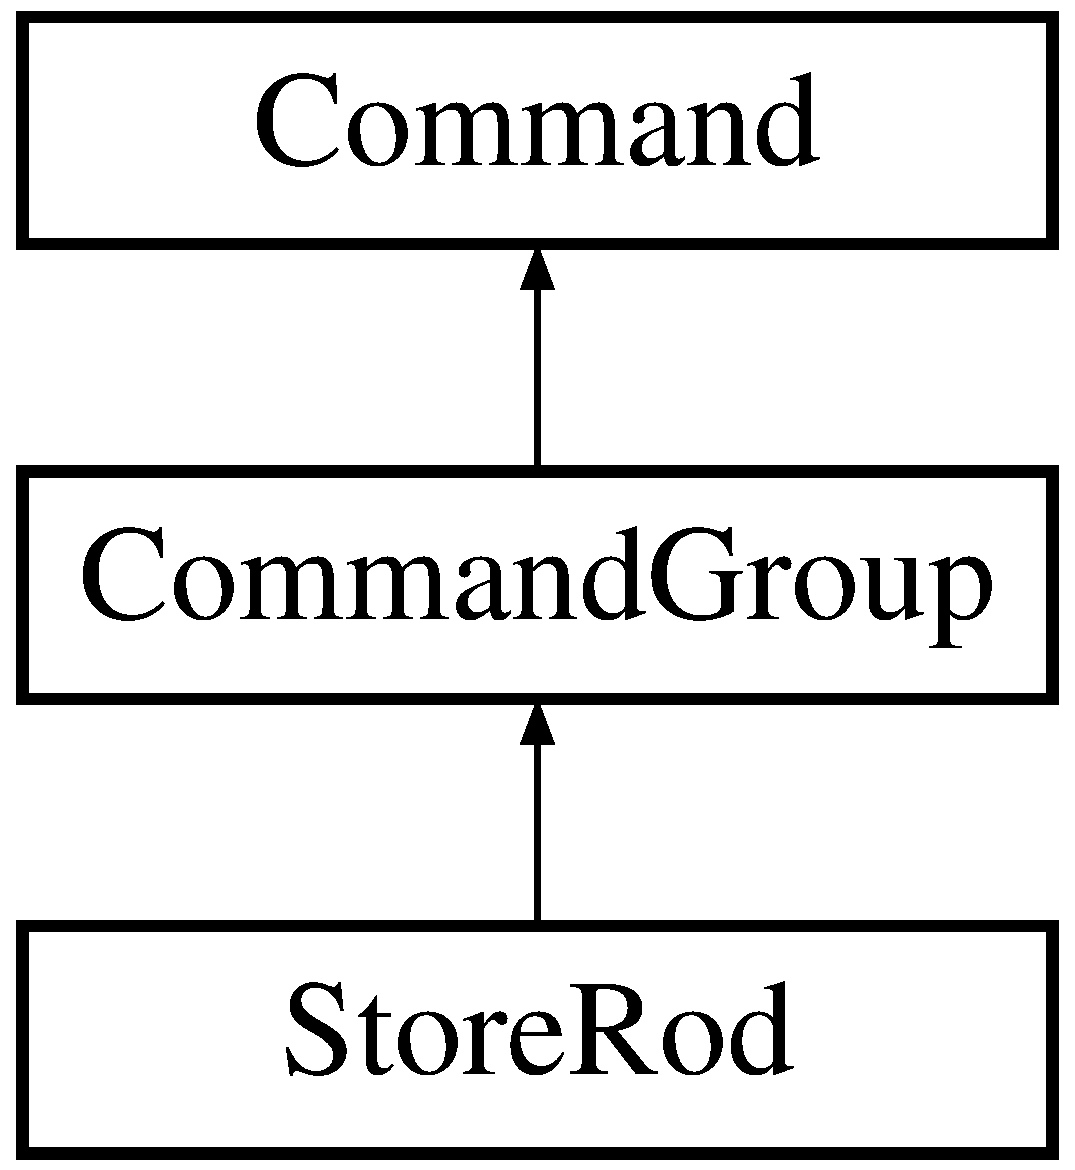
\includegraphics[height=3.000000cm]{classStoreRod}
\end{center}
\end{figure}
\subsection*{Additional Inherited Members}


The documentation for this class was generated from the following files\-:\begin{DoxyCompactItemize}
\item 
Final\-\_\-\-Project/Store\-Rod.\-h\item 
Final\-\_\-\-Project/Store\-Rod.\-cpp\end{DoxyCompactItemize}

\hypertarget{classStoreRodInReactor}{\section{Store\-Rod\-In\-Reactor Class Reference}
\label{classStoreRodInReactor}\index{Store\-Rod\-In\-Reactor@{Store\-Rod\-In\-Reactor}}
}


puts the rod into the reactor specified  




{\ttfamily \#include $<$Store\-Rod\-In\-Reactor.\-h$>$}

Inheritance diagram for Store\-Rod\-In\-Reactor\-:\begin{figure}[H]
\begin{center}
\leavevmode
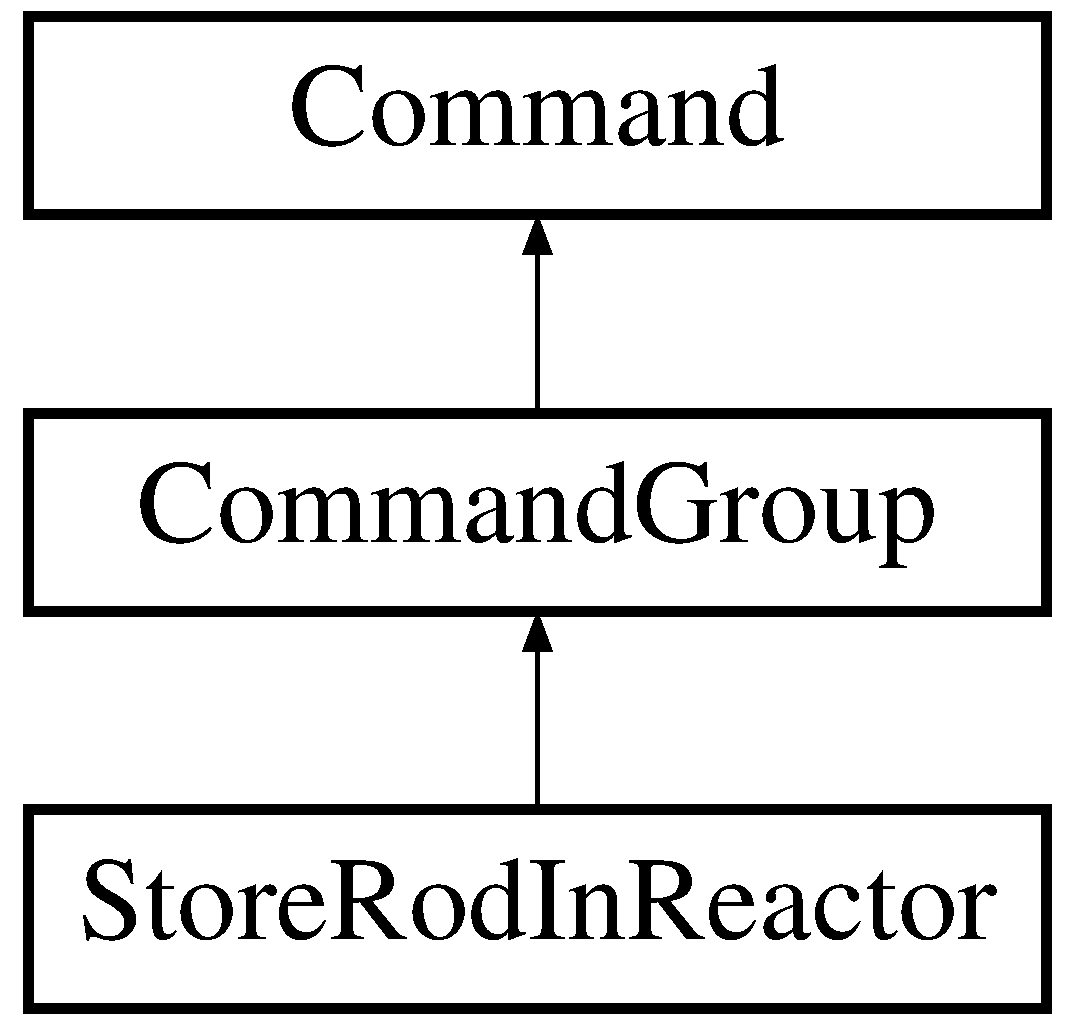
\includegraphics[height=3.000000cm]{classStoreRodInReactor}
\end{center}
\end{figure}
\subsection*{Public Member Functions}
\begin{DoxyCompactItemize}
\item 
\hyperlink{classStoreRodInReactor_a1a72a4e2f134e009b8c911efd4ced737}{Store\-Rod\-In\-Reactor} (const int \hyperlink{classStoreRodInReactor_a5d989548741b48953a5bb4e20f294d72}{reactor\-Number})
\item 
void \hyperlink{classStoreRodInReactor_aa315630b1fcbb752dcc7f6425c96959f}{initialize} ()
\begin{DoxyCompactList}\small\item\em run once in the first iteration of the command's life. this will be overrided by individual commands \end{DoxyCompactList}\item 
void \hyperlink{classStoreRodInReactor_a39f60444f52164e7405331e61b050e83}{end} ()
\begin{DoxyCompactList}\small\item\em called once at the end, once \hyperlink{classCommandGroup_a96807a2763adf9e21ebf2cb9e3574e3c}{is\-Finished()} returned true. this will be overrided by individual commands. \end{DoxyCompactList}\end{DoxyCompactItemize}
\subsection*{Private Attributes}
\begin{DoxyCompactItemize}
\item 
int \hyperlink{classStoreRodInReactor_a5d989548741b48953a5bb4e20f294d72}{reactor\-Number}
\end{DoxyCompactItemize}
\subsection*{Additional Inherited Members}


\subsection{Detailed Description}
puts the rod into the reactor specified 

Definition at line 8 of file Store\-Rod\-In\-Reactor.\-h.



\subsection{Constructor \& Destructor Documentation}
\hypertarget{classStoreRodInReactor_a1a72a4e2f134e009b8c911efd4ced737}{\index{Store\-Rod\-In\-Reactor@{Store\-Rod\-In\-Reactor}!Store\-Rod\-In\-Reactor@{Store\-Rod\-In\-Reactor}}
\index{Store\-Rod\-In\-Reactor@{Store\-Rod\-In\-Reactor}!StoreRodInReactor@{Store\-Rod\-In\-Reactor}}
\subsubsection[{Store\-Rod\-In\-Reactor}]{\setlength{\rightskip}{0pt plus 5cm}Store\-Rod\-In\-Reactor\-::\-Store\-Rod\-In\-Reactor (
\begin{DoxyParamCaption}
\item[{const int}]{reactor\-Number}
\end{DoxyParamCaption}
)}}\label{classStoreRodInReactor_a1a72a4e2f134e009b8c911efd4ced737}


Definition at line 9 of file Store\-Rod\-In\-Reactor.\-cpp.



\subsection{Member Function Documentation}
\hypertarget{classStoreRodInReactor_a39f60444f52164e7405331e61b050e83}{\index{Store\-Rod\-In\-Reactor@{Store\-Rod\-In\-Reactor}!end@{end}}
\index{end@{end}!StoreRodInReactor@{Store\-Rod\-In\-Reactor}}
\subsubsection[{end}]{\setlength{\rightskip}{0pt plus 5cm}void Store\-Rod\-In\-Reactor\-::end (
\begin{DoxyParamCaption}
{}
\end{DoxyParamCaption}
)\hspace{0.3cm}{\ttfamily [virtual]}}}\label{classStoreRodInReactor_a39f60444f52164e7405331e61b050e83}


called once at the end, once \hyperlink{classCommandGroup_a96807a2763adf9e21ebf2cb9e3574e3c}{is\-Finished()} returned true. this will be overrided by individual commands. 



Reimplemented from \hyperlink{classCommandGroup_a28ad3a1c2f6b4f9aea10efa1a824895e}{Command\-Group}.



Definition at line 33 of file Store\-Rod\-In\-Reactor.\-cpp.

\hypertarget{classStoreRodInReactor_aa315630b1fcbb752dcc7f6425c96959f}{\index{Store\-Rod\-In\-Reactor@{Store\-Rod\-In\-Reactor}!initialize@{initialize}}
\index{initialize@{initialize}!StoreRodInReactor@{Store\-Rod\-In\-Reactor}}
\subsubsection[{initialize}]{\setlength{\rightskip}{0pt plus 5cm}void Store\-Rod\-In\-Reactor\-::initialize (
\begin{DoxyParamCaption}
{}
\end{DoxyParamCaption}
)\hspace{0.3cm}{\ttfamily [virtual]}}}\label{classStoreRodInReactor_aa315630b1fcbb752dcc7f6425c96959f}


run once in the first iteration of the command's life. this will be overrided by individual commands 



Reimplemented from \hyperlink{classCommandGroup_a99800c5dbd05ab750aa0bb27518d0467}{Command\-Group}.



Definition at line 13 of file Store\-Rod\-In\-Reactor.\-cpp.



\subsection{Member Data Documentation}
\hypertarget{classStoreRodInReactor_a5d989548741b48953a5bb4e20f294d72}{\index{Store\-Rod\-In\-Reactor@{Store\-Rod\-In\-Reactor}!reactor\-Number@{reactor\-Number}}
\index{reactor\-Number@{reactor\-Number}!StoreRodInReactor@{Store\-Rod\-In\-Reactor}}
\subsubsection[{reactor\-Number}]{\setlength{\rightskip}{0pt plus 5cm}int Store\-Rod\-In\-Reactor\-::reactor\-Number\hspace{0.3cm}{\ttfamily [private]}}}\label{classStoreRodInReactor_a5d989548741b48953a5bb4e20f294d72}


Definition at line 14 of file Store\-Rod\-In\-Reactor.\-h.



The documentation for this class was generated from the following files\-:\begin{DoxyCompactItemize}
\item 
Final\-\_\-\-Project/\hyperlink{StoreRodInReactor_8h}{Store\-Rod\-In\-Reactor.\-h}\item 
Final\-\_\-\-Project/\hyperlink{StoreRodInReactor_8cpp}{Store\-Rod\-In\-Reactor.\-cpp}\end{DoxyCompactItemize}

\hypertarget{classTurn}{\section{Turn Class Reference}
\label{classTurn}\index{Turn@{Turn}}
}
Inheritance diagram for Turn\-:\begin{figure}[H]
\begin{center}
\leavevmode
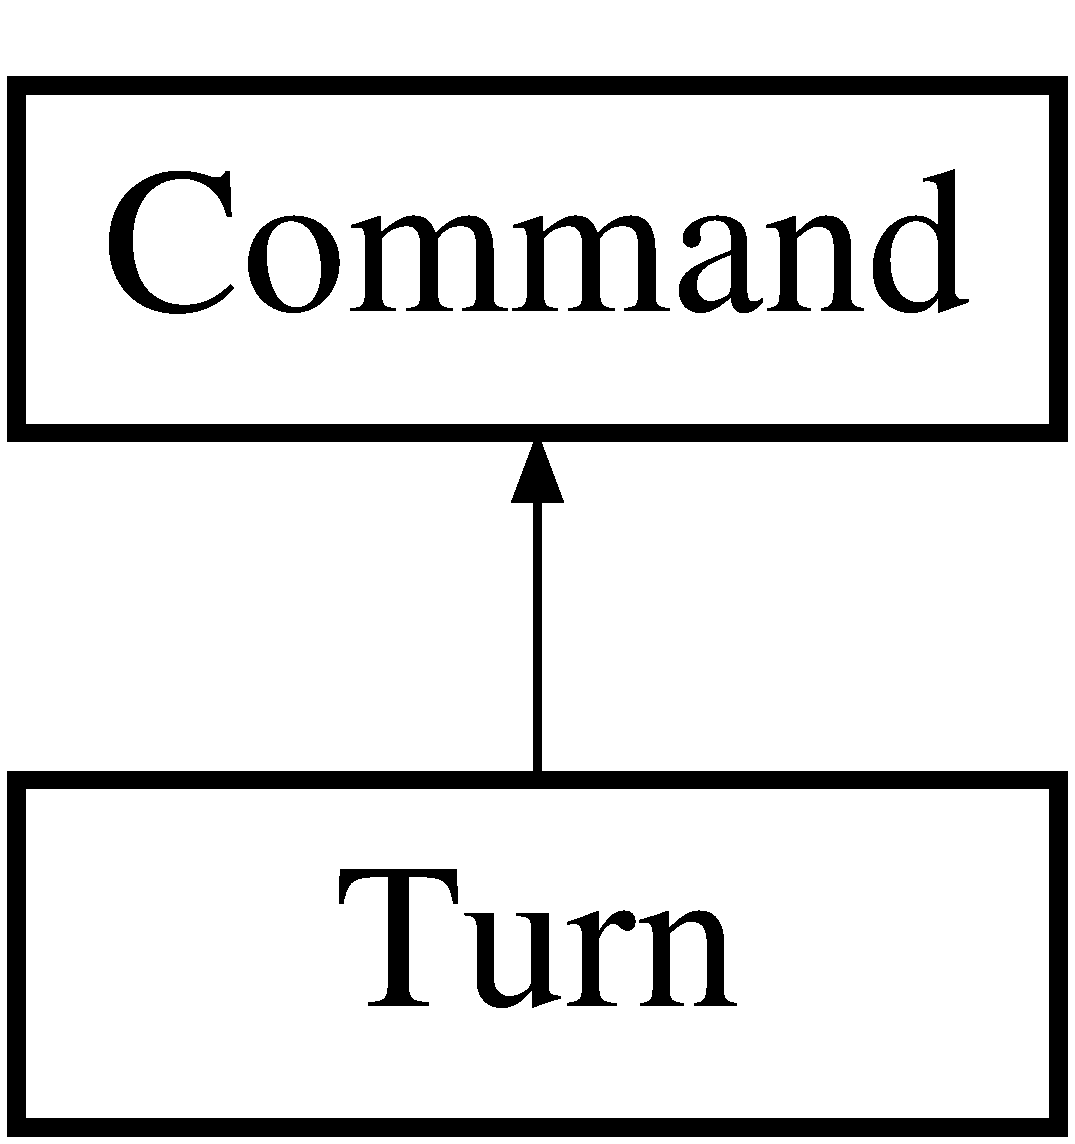
\includegraphics[height=2.000000cm]{classTurn}
\end{center}
\end{figure}
\subsection*{Public Member Functions}
\begin{DoxyCompactItemize}
\item 
\hypertarget{classTurn_a4a9fef27d1f57956ea4d50983d35294b}{{\bfseries Turn} (int direction, int timeout)}\label{classTurn_a4a9fef27d1f57956ea4d50983d35294b}

\item 
\hypertarget{classTurn_a5eb51a7d1c2776461f26019fb010c69b}{void \hyperlink{classTurn_a5eb51a7d1c2776461f26019fb010c69b}{initialize} ()}\label{classTurn_a5eb51a7d1c2776461f26019fb010c69b}

\begin{DoxyCompactList}\small\item\em run once in the first iteration of the command's life. this will be overrided by individual commands \end{DoxyCompactList}\item 
\hypertarget{classTurn_a93e23ddc414f55d3f52eb71d7d06d3d9}{void \hyperlink{classTurn_a93e23ddc414f55d3f52eb71d7d06d3d9}{execute} ()}\label{classTurn_a93e23ddc414f55d3f52eb71d7d06d3d9}

\begin{DoxyCompactList}\small\item\em stuff to do over and over each iteration. this will be overrided by individual commands \end{DoxyCompactList}\item 
bool \hyperlink{classTurn_af7420468ed671ef0d1db487361f0bf41}{is\-Finished} ()
\begin{DoxyCompactList}\small\item\em checked every iteration to see if we're done here. this will be overrided by individual commands \end{DoxyCompactList}\item 
\hypertarget{classTurn_a3fc900a7951717778569127d978ba236}{void \hyperlink{classTurn_a3fc900a7951717778569127d978ba236}{end} ()}\label{classTurn_a3fc900a7951717778569127d978ba236}

\begin{DoxyCompactList}\small\item\em called once at the end, once \hyperlink{classTurn_af7420468ed671ef0d1db487361f0bf41}{is\-Finished()} returned true. this will be overrided by individual commands. \end{DoxyCompactList}\end{DoxyCompactItemize}
\subsection*{Additional Inherited Members}


\subsection{Member Function Documentation}
\hypertarget{classTurn_af7420468ed671ef0d1db487361f0bf41}{\index{Turn@{Turn}!is\-Finished@{is\-Finished}}
\index{is\-Finished@{is\-Finished}!Turn@{Turn}}
\subsubsection[{is\-Finished}]{\setlength{\rightskip}{0pt plus 5cm}bool Turn\-::is\-Finished (
\begin{DoxyParamCaption}
{}
\end{DoxyParamCaption}
)\hspace{0.3cm}{\ttfamily [virtual]}}}\label{classTurn_af7420468ed671ef0d1db487361f0bf41}


checked every iteration to see if we're done here. this will be overrided by individual commands 

\begin{DoxyReturn}{Returns}
is the function finished 
\end{DoxyReturn}


Implements \hyperlink{classCommand_a9aa704d5f9d98f510a79e645701dc72a}{Command}.



The documentation for this class was generated from the following files\-:\begin{DoxyCompactItemize}
\item 
Final\-\_\-\-Project/Turn.\-h\item 
Final\-\_\-\-Project/Turn.\-cpp\end{DoxyCompactItemize}

\hypertarget{classTurnAround}{\section{Turn\-Around Class Reference}
\label{classTurnAround}\index{Turn\-Around@{Turn\-Around}}
}
Inheritance diagram for Turn\-Around\-:\begin{figure}[H]
\begin{center}
\leavevmode
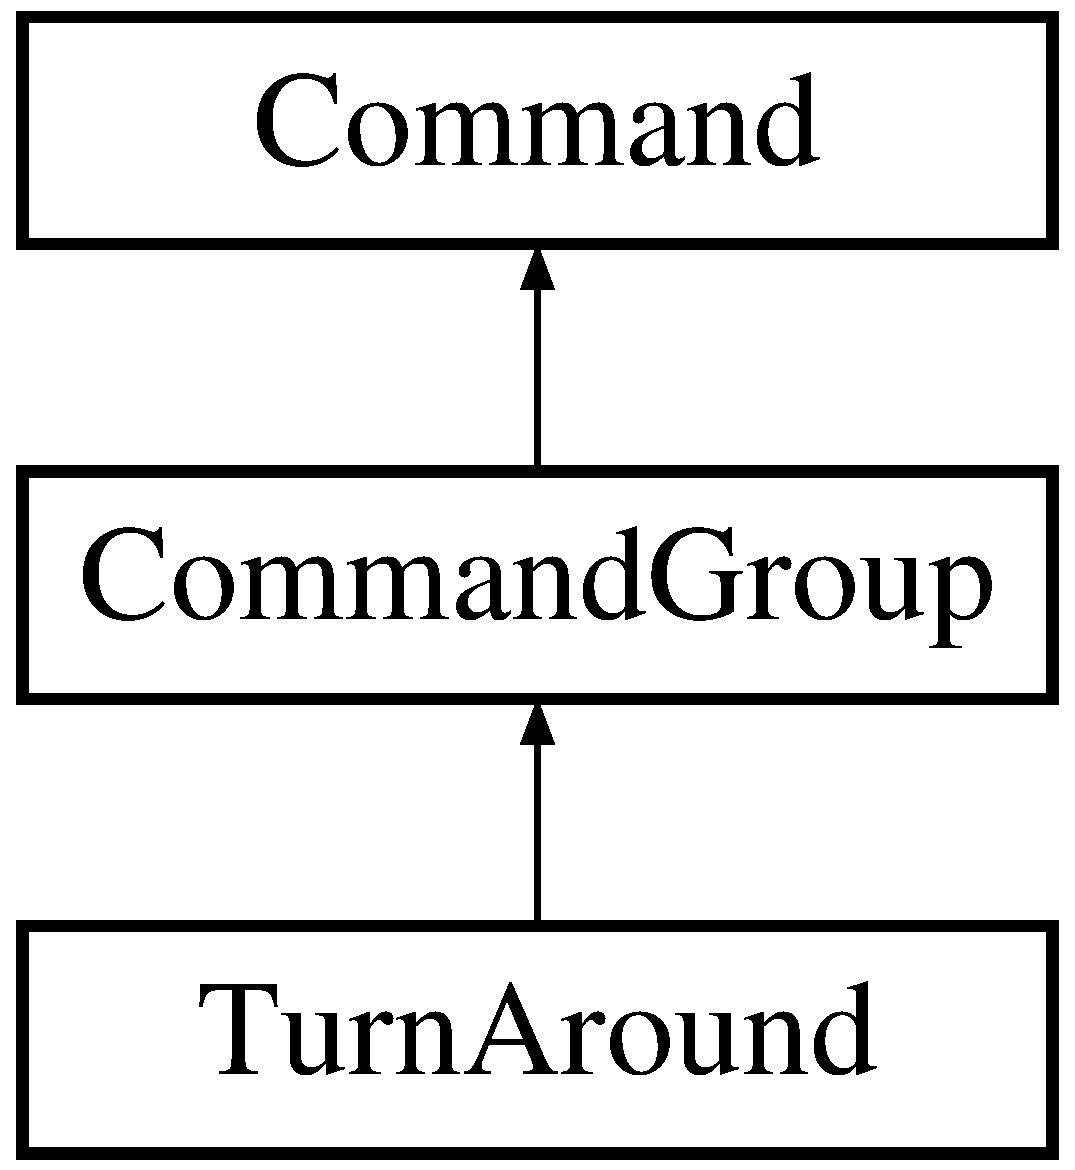
\includegraphics[height=3.000000cm]{classTurnAround}
\end{center}
\end{figure}
\subsection*{Additional Inherited Members}


The documentation for this class was generated from the following file\-:\begin{DoxyCompactItemize}
\item 
Final\-\_\-\-Project/Turn\-Around.\-h\end{DoxyCompactItemize}

\hypertarget{classTurnOffLine}{\section{Turn\-Off\-Line Class Reference}
\label{classTurnOffLine}\index{Turn\-Off\-Line@{Turn\-Off\-Line}}
}


turns off of the line in a direction  




{\ttfamily \#include $<$Turn\-Off\-Line.\-h$>$}

Inheritance diagram for Turn\-Off\-Line\-:\begin{figure}[H]
\begin{center}
\leavevmode
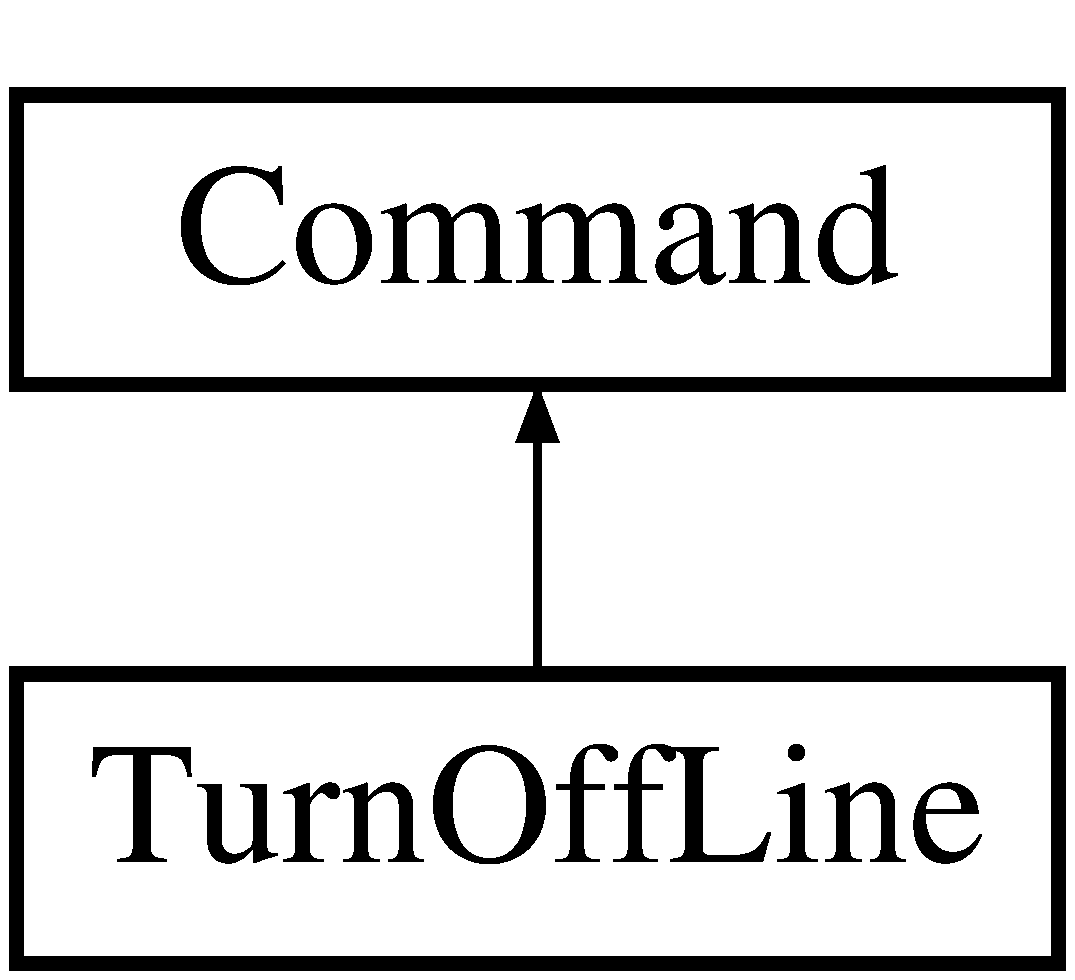
\includegraphics[height=2.000000cm]{classTurnOffLine}
\end{center}
\end{figure}
\subsection*{Public Member Functions}
\begin{DoxyCompactItemize}
\item 
\hyperlink{classTurnOffLine_a646faf11da687b4ed4330c6248b6e99e}{Turn\-Off\-Line} (int \hyperlink{classTurnOffLine_a7f229d3b3f2e9707b550affb60e7a71a}{direction})
\item 
void \hyperlink{classTurnOffLine_a4072817ff86f237d276a430e56e912a3}{initialize} ()
\begin{DoxyCompactList}\small\item\em sets a timeout and plays a song \end{DoxyCompactList}\item 
virtual void \hyperlink{classTurnOffLine_a9897de245832cd3ee74edc35b342fc03}{execute} ()
\begin{DoxyCompactList}\small\item\em determines the direction then turns that direction \end{DoxyCompactList}\item 
bool \hyperlink{classTurnOffLine_ad924499a6bc07a7331222e9b4aba3517}{is\-Finished} ()
\item 
virtual void \hyperlink{classTurnOffLine_ad888d865fb75e8139825f4dcf7709f1e}{end} ()
\begin{DoxyCompactList}\small\item\em stops the robot \end{DoxyCompactList}\end{DoxyCompactItemize}
\subsection*{Private Attributes}
\begin{DoxyCompactItemize}
\item 
int \hyperlink{classTurnOffLine_a7f229d3b3f2e9707b550affb60e7a71a}{direction}
\begin{DoxyCompactList}\small\item\em direction specified by bluetooth \end{DoxyCompactList}\end{DoxyCompactItemize}
\subsection*{Additional Inherited Members}


\subsection{Detailed Description}
turns off of the line in a direction 

Definition at line 8 of file Turn\-Off\-Line.\-h.



\subsection{Constructor \& Destructor Documentation}
\hypertarget{classTurnOffLine_a646faf11da687b4ed4330c6248b6e99e}{\index{Turn\-Off\-Line@{Turn\-Off\-Line}!Turn\-Off\-Line@{Turn\-Off\-Line}}
\index{Turn\-Off\-Line@{Turn\-Off\-Line}!TurnOffLine@{Turn\-Off\-Line}}
\subsubsection[{Turn\-Off\-Line}]{\setlength{\rightskip}{0pt plus 5cm}Turn\-Off\-Line\-::\-Turn\-Off\-Line (
\begin{DoxyParamCaption}
\item[{int}]{direction}
\end{DoxyParamCaption}
)}}\label{classTurnOffLine_a646faf11da687b4ed4330c6248b6e99e}

\begin{DoxyParams}{Parameters}
{\em direction} & specified by bluetooth, either ccw or cw \\
\hline
\end{DoxyParams}


Definition at line 4 of file Turn\-Off\-Line.\-cpp.



\subsection{Member Function Documentation}
\hypertarget{classTurnOffLine_ad888d865fb75e8139825f4dcf7709f1e}{\index{Turn\-Off\-Line@{Turn\-Off\-Line}!end@{end}}
\index{end@{end}!TurnOffLine@{Turn\-Off\-Line}}
\subsubsection[{end}]{\setlength{\rightskip}{0pt plus 5cm}void Turn\-Off\-Line\-::end (
\begin{DoxyParamCaption}
{}
\end{DoxyParamCaption}
)\hspace{0.3cm}{\ttfamily [virtual]}}}\label{classTurnOffLine_ad888d865fb75e8139825f4dcf7709f1e}


stops the robot 



Reimplemented from \hyperlink{classCommand_a147da4a43c939870018324a0af4c7b0b}{Command}.



Definition at line 26 of file Turn\-Off\-Line.\-cpp.

\hypertarget{classTurnOffLine_a9897de245832cd3ee74edc35b342fc03}{\index{Turn\-Off\-Line@{Turn\-Off\-Line}!execute@{execute}}
\index{execute@{execute}!TurnOffLine@{Turn\-Off\-Line}}
\subsubsection[{execute}]{\setlength{\rightskip}{0pt plus 5cm}void Turn\-Off\-Line\-::execute (
\begin{DoxyParamCaption}
{}
\end{DoxyParamCaption}
)\hspace{0.3cm}{\ttfamily [virtual]}}}\label{classTurnOffLine_a9897de245832cd3ee74edc35b342fc03}


determines the direction then turns that direction 



Reimplemented from \hyperlink{classCommand_abc8574913684044b0f1a9f810b4e969b}{Command}.



Definition at line 13 of file Turn\-Off\-Line.\-cpp.

\hypertarget{classTurnOffLine_a4072817ff86f237d276a430e56e912a3}{\index{Turn\-Off\-Line@{Turn\-Off\-Line}!initialize@{initialize}}
\index{initialize@{initialize}!TurnOffLine@{Turn\-Off\-Line}}
\subsubsection[{initialize}]{\setlength{\rightskip}{0pt plus 5cm}void Turn\-Off\-Line\-::initialize (
\begin{DoxyParamCaption}
{}
\end{DoxyParamCaption}
)\hspace{0.3cm}{\ttfamily [virtual]}}}\label{classTurnOffLine_a4072817ff86f237d276a430e56e912a3}


sets a timeout and plays a song 



Reimplemented from \hyperlink{classCommand_a8044ac332a61df571c3454d9fea9684a}{Command}.



Definition at line 8 of file Turn\-Off\-Line.\-cpp.

\hypertarget{classTurnOffLine_ad924499a6bc07a7331222e9b4aba3517}{\index{Turn\-Off\-Line@{Turn\-Off\-Line}!is\-Finished@{is\-Finished}}
\index{is\-Finished@{is\-Finished}!TurnOffLine@{Turn\-Off\-Line}}
\subsubsection[{is\-Finished}]{\setlength{\rightskip}{0pt plus 5cm}bool Turn\-Off\-Line\-::is\-Finished (
\begin{DoxyParamCaption}
{}
\end{DoxyParamCaption}
)\hspace{0.3cm}{\ttfamily [virtual]}}}\label{classTurnOffLine_ad924499a6bc07a7331222e9b4aba3517}
\begin{DoxyReturn}{Returns}
true when timeout occurs 
\end{DoxyReturn}


Reimplemented from \hyperlink{classCommand_ae5846b4332a262e055c7a96759fa18f2}{Command}.



Definition at line 22 of file Turn\-Off\-Line.\-cpp.



\subsection{Member Data Documentation}
\hypertarget{classTurnOffLine_a7f229d3b3f2e9707b550affb60e7a71a}{\index{Turn\-Off\-Line@{Turn\-Off\-Line}!direction@{direction}}
\index{direction@{direction}!TurnOffLine@{Turn\-Off\-Line}}
\subsubsection[{direction}]{\setlength{\rightskip}{0pt plus 5cm}int Turn\-Off\-Line\-::direction\hspace{0.3cm}{\ttfamily [private]}}}\label{classTurnOffLine_a7f229d3b3f2e9707b550affb60e7a71a}


direction specified by bluetooth 



Definition at line 37 of file Turn\-Off\-Line.\-h.



The documentation for this class was generated from the following files\-:\begin{DoxyCompactItemize}
\item 
Final\-\_\-\-Project/\hyperlink{TurnOffLine_8h}{Turn\-Off\-Line.\-h}\item 
Final\-\_\-\-Project/\hyperlink{TurnOffLine_8cpp}{Turn\-Off\-Line.\-cpp}\end{DoxyCompactItemize}

\hypertarget{classTurnToFace}{\section{Turn\-To\-Face Class Reference}
\label{classTurnToFace}\index{Turn\-To\-Face@{Turn\-To\-Face}}
}
Inheritance diagram for Turn\-To\-Face\-:\begin{figure}[H]
\begin{center}
\leavevmode
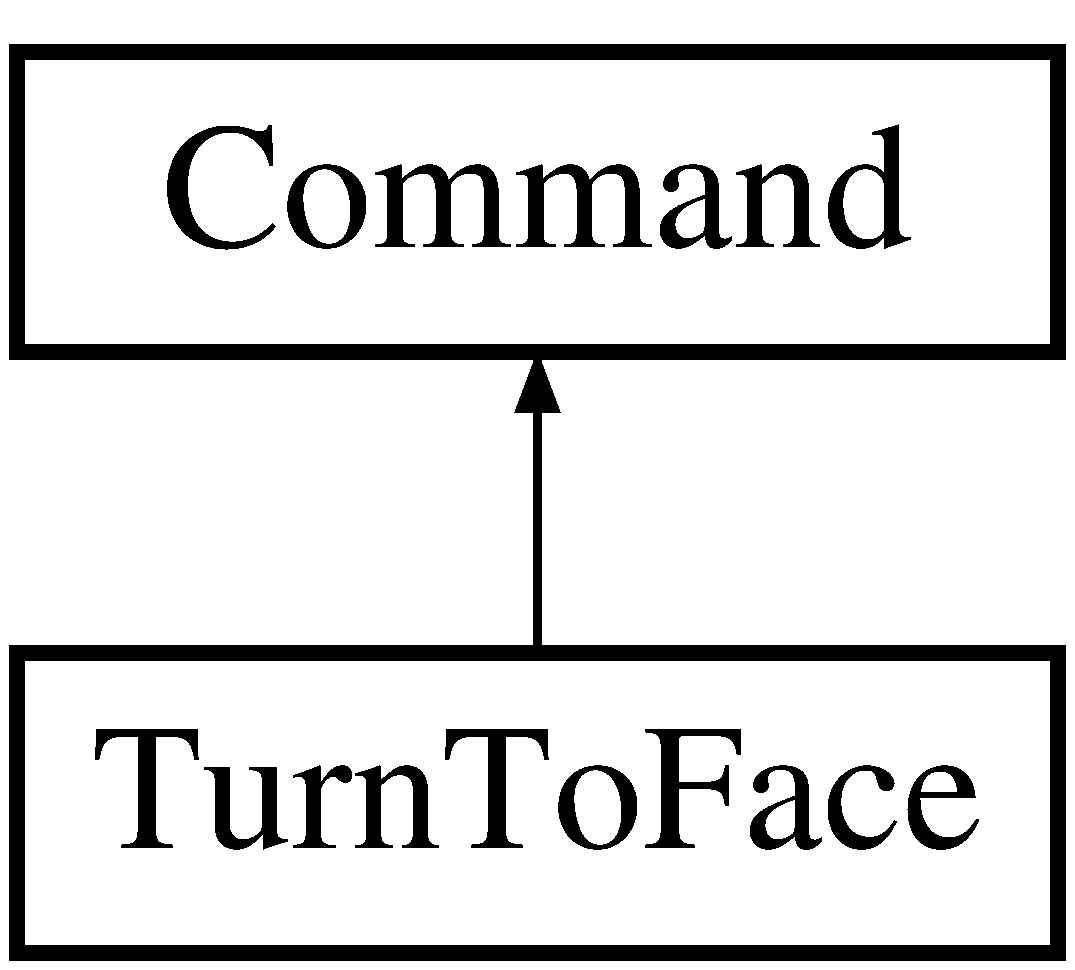
\includegraphics[height=2.000000cm]{classTurnToFace}
\end{center}
\end{figure}
\subsection*{Public Member Functions}
\begin{DoxyCompactItemize}
\item 
\hypertarget{classTurnToFace_ada3a9e946f131ad12ce46373dbd38890}{{\bfseries Turn\-To\-Face} (int dest\-Direction)}\label{classTurnToFace_ada3a9e946f131ad12ce46373dbd38890}

\item 
\hypertarget{classTurnToFace_a4e4583374430f20b1104fdc177275cf7}{void \hyperlink{classTurnToFace_a4e4583374430f20b1104fdc177275cf7}{initialize} ()}\label{classTurnToFace_a4e4583374430f20b1104fdc177275cf7}

\begin{DoxyCompactList}\small\item\em run once in the first iteration of the command's life. this will be overrided by individual commands \end{DoxyCompactList}\item 
\hypertarget{classTurnToFace_a7b051988a247f6be7cfaaebe09215c78}{void \hyperlink{classTurnToFace_a7b051988a247f6be7cfaaebe09215c78}{execute} ()}\label{classTurnToFace_a7b051988a247f6be7cfaaebe09215c78}

\begin{DoxyCompactList}\small\item\em stuff to do over and over each iteration. this will be overrided by individual commands \end{DoxyCompactList}\item 
bool \hyperlink{classTurnToFace_afd6933d5eca23dcd3c4f95c7528c6fe6}{is\-Finished} ()
\begin{DoxyCompactList}\small\item\em checked every iteration to see if we're done here. this will be overrided by individual commands \end{DoxyCompactList}\item 
\hypertarget{classTurnToFace_a13de7c83710f05d7343b85ba73522f27}{void \hyperlink{classTurnToFace_a13de7c83710f05d7343b85ba73522f27}{end} ()}\label{classTurnToFace_a13de7c83710f05d7343b85ba73522f27}

\begin{DoxyCompactList}\small\item\em called once at the end, once \hyperlink{classTurnToFace_afd6933d5eca23dcd3c4f95c7528c6fe6}{is\-Finished()} returned true. this will be overrided by individual commands. \end{DoxyCompactList}\end{DoxyCompactItemize}
\subsection*{Additional Inherited Members}


\subsection{Member Function Documentation}
\hypertarget{classTurnToFace_afd6933d5eca23dcd3c4f95c7528c6fe6}{\index{Turn\-To\-Face@{Turn\-To\-Face}!is\-Finished@{is\-Finished}}
\index{is\-Finished@{is\-Finished}!TurnToFace@{Turn\-To\-Face}}
\subsubsection[{is\-Finished}]{\setlength{\rightskip}{0pt plus 5cm}bool Turn\-To\-Face\-::is\-Finished (
\begin{DoxyParamCaption}
{}
\end{DoxyParamCaption}
)\hspace{0.3cm}{\ttfamily [virtual]}}}\label{classTurnToFace_afd6933d5eca23dcd3c4f95c7528c6fe6}


checked every iteration to see if we're done here. this will be overrided by individual commands 

\begin{DoxyReturn}{Returns}
is the function finished 
\end{DoxyReturn}


Implements \hyperlink{classCommand_a9aa704d5f9d98f510a79e645701dc72a}{Command}.



The documentation for this class was generated from the following files\-:\begin{DoxyCompactItemize}
\item 
Final\-\_\-\-Project/Turn\-To\-Face.\-h\item 
Final\-\_\-\-Project/Turn\-To\-Face.\-cpp\end{DoxyCompactItemize}

\hypertarget{classTurnUntilLine}{\section{Turn\-Until\-Line Class Reference}
\label{classTurnUntilLine}\index{Turn\-Until\-Line@{Turn\-Until\-Line}}
}


{\ttfamily \#include $<$Turn\-Until\-Line.\-h$>$}

Inheritance diagram for Turn\-Until\-Line\-:\begin{figure}[H]
\begin{center}
\leavevmode
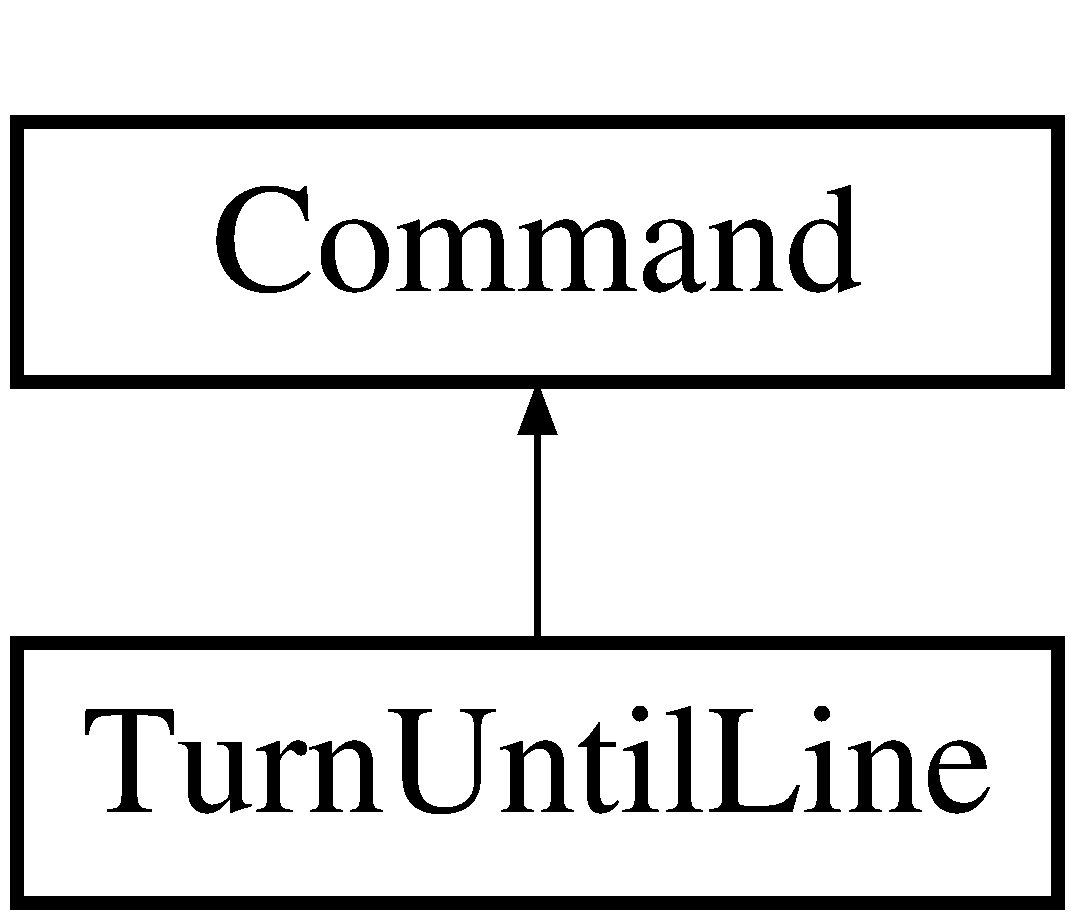
\includegraphics[height=2.000000cm]{classTurnUntilLine}
\end{center}
\end{figure}
\subsection*{Public Member Functions}
\begin{DoxyCompactItemize}
\item 
\hyperlink{classTurnUntilLine_a737bfe72e0d4dbcce9f91182e319d28d}{Turn\-Until\-Line} (int \hyperlink{classTurnUntilLine_ac7e62d06dece2d456f9ea6e987b480cf}{direction})
\begin{DoxyCompactList}\small\item\em turns until the line sensor is on line \end{DoxyCompactList}\item 
void \hyperlink{classTurnUntilLine_a99e42f7512b95097df29633877e72cbd}{initialize} ()
\begin{DoxyCompactList}\small\item\em plays a song \end{DoxyCompactList}\item 
void \hyperlink{classTurnUntilLine_a90feb7840ebc51984e4d0a31383ec5a9}{execute} ()
\begin{DoxyCompactList}\small\item\em rotates either ccw or cw \end{DoxyCompactList}\item 
bool \hyperlink{classTurnUntilLine_ad9232508d735c78d6443958fe2f18002}{is\-Finished} ()
\item 
void \hyperlink{classTurnUntilLine_a769864873e706e0ca6701eac7f947ede}{end} ()
\end{DoxyCompactItemize}
\subsection*{Private Attributes}
\begin{DoxyCompactItemize}
\item 
int \hyperlink{classTurnUntilLine_ac7e62d06dece2d456f9ea6e987b480cf}{direction}
\begin{DoxyCompactList}\small\item\em this is the direction used to determine turn direction \end{DoxyCompactList}\end{DoxyCompactItemize}
\subsection*{Additional Inherited Members}


\subsection{Detailed Description}
/brief turns until it hits a line 

Definition at line 8 of file Turn\-Until\-Line.\-h.



\subsection{Constructor \& Destructor Documentation}
\hypertarget{classTurnUntilLine_a737bfe72e0d4dbcce9f91182e319d28d}{\index{Turn\-Until\-Line@{Turn\-Until\-Line}!Turn\-Until\-Line@{Turn\-Until\-Line}}
\index{Turn\-Until\-Line@{Turn\-Until\-Line}!TurnUntilLine@{Turn\-Until\-Line}}
\subsubsection[{Turn\-Until\-Line}]{\setlength{\rightskip}{0pt plus 5cm}Turn\-Until\-Line\-::\-Turn\-Until\-Line (
\begin{DoxyParamCaption}
\item[{int}]{direction}
\end{DoxyParamCaption}
)}}\label{classTurnUntilLine_a737bfe72e0d4dbcce9f91182e319d28d}


turns until the line sensor is on line 



Definition at line 4 of file Turn\-Until\-Line.\-cpp.



\subsection{Member Function Documentation}
\hypertarget{classTurnUntilLine_a769864873e706e0ca6701eac7f947ede}{\index{Turn\-Until\-Line@{Turn\-Until\-Line}!end@{end}}
\index{end@{end}!TurnUntilLine@{Turn\-Until\-Line}}
\subsubsection[{end}]{\setlength{\rightskip}{0pt plus 5cm}void Turn\-Until\-Line\-::end (
\begin{DoxyParamCaption}
{}
\end{DoxyParamCaption}
)\hspace{0.3cm}{\ttfamily [virtual]}}}\label{classTurnUntilLine_a769864873e706e0ca6701eac7f947ede}
stops robot 

Reimplemented from \hyperlink{classCommand_a147da4a43c939870018324a0af4c7b0b}{Command}.



Definition at line 30 of file Turn\-Until\-Line.\-cpp.

\hypertarget{classTurnUntilLine_a90feb7840ebc51984e4d0a31383ec5a9}{\index{Turn\-Until\-Line@{Turn\-Until\-Line}!execute@{execute}}
\index{execute@{execute}!TurnUntilLine@{Turn\-Until\-Line}}
\subsubsection[{execute}]{\setlength{\rightskip}{0pt plus 5cm}void Turn\-Until\-Line\-::execute (
\begin{DoxyParamCaption}
{}
\end{DoxyParamCaption}
)\hspace{0.3cm}{\ttfamily [virtual]}}}\label{classTurnUntilLine_a90feb7840ebc51984e4d0a31383ec5a9}


rotates either ccw or cw 



Reimplemented from \hyperlink{classCommand_abc8574913684044b0f1a9f810b4e969b}{Command}.



Definition at line 12 of file Turn\-Until\-Line.\-cpp.

\hypertarget{classTurnUntilLine_a99e42f7512b95097df29633877e72cbd}{\index{Turn\-Until\-Line@{Turn\-Until\-Line}!initialize@{initialize}}
\index{initialize@{initialize}!TurnUntilLine@{Turn\-Until\-Line}}
\subsubsection[{initialize}]{\setlength{\rightskip}{0pt plus 5cm}void Turn\-Until\-Line\-::initialize (
\begin{DoxyParamCaption}
{}
\end{DoxyParamCaption}
)\hspace{0.3cm}{\ttfamily [virtual]}}}\label{classTurnUntilLine_a99e42f7512b95097df29633877e72cbd}


plays a song 



Reimplemented from \hyperlink{classCommand_a8044ac332a61df571c3454d9fea9684a}{Command}.



Definition at line 8 of file Turn\-Until\-Line.\-cpp.

\hypertarget{classTurnUntilLine_ad9232508d735c78d6443958fe2f18002}{\index{Turn\-Until\-Line@{Turn\-Until\-Line}!is\-Finished@{is\-Finished}}
\index{is\-Finished@{is\-Finished}!TurnUntilLine@{Turn\-Until\-Line}}
\subsubsection[{is\-Finished}]{\setlength{\rightskip}{0pt plus 5cm}bool Turn\-Until\-Line\-::is\-Finished (
\begin{DoxyParamCaption}
{}
\end{DoxyParamCaption}
)\hspace{0.3cm}{\ttfamily [virtual]}}}\label{classTurnUntilLine_ad9232508d735c78d6443958fe2f18002}
\begin{DoxyReturn}{Returns}
true if robot is on line 
\end{DoxyReturn}


Reimplemented from \hyperlink{classCommand_ae5846b4332a262e055c7a96759fa18f2}{Command}.



Definition at line 21 of file Turn\-Until\-Line.\-cpp.



\subsection{Member Data Documentation}
\hypertarget{classTurnUntilLine_ac7e62d06dece2d456f9ea6e987b480cf}{\index{Turn\-Until\-Line@{Turn\-Until\-Line}!direction@{direction}}
\index{direction@{direction}!TurnUntilLine@{Turn\-Until\-Line}}
\subsubsection[{direction}]{\setlength{\rightskip}{0pt plus 5cm}int Turn\-Until\-Line\-::direction\hspace{0.3cm}{\ttfamily [private]}}}\label{classTurnUntilLine_ac7e62d06dece2d456f9ea6e987b480cf}


this is the direction used to determine turn direction 



Definition at line 38 of file Turn\-Until\-Line.\-h.



The documentation for this class was generated from the following files\-:\begin{DoxyCompactItemize}
\item 
Final\-\_\-\-Project/\hyperlink{TurnUntilLine_8h}{Turn\-Until\-Line.\-h}\item 
Final\-\_\-\-Project/\hyperlink{TurnUntilLine_8cpp}{Turn\-Until\-Line.\-cpp}\end{DoxyCompactItemize}

%--- End generated contents ---

% Index
\newpage
\phantomsection
\addcontentsline{toc}{chapter}{Index}
\printindex

\end{document}
